\newcommand{\documenttitle}{Norme di Progetto}
\newcommand{\addressedto}{\committente \\ & \committenteAlt}
\newcommand{\editorialstaff}{\sm}
\newcommand{\teststaff}{\ao}
\newcommand{\approvalstaff}{\dm}
\newcommand{\use}{Interno}
\documentclass[a4paper,11pt]{article}

\usepackage[italian]{babel}
\usepackage[utf8]{inputenc} % permette l'inserimento di caratteri accentati da tastiera nel documento sorgente.
\usepackage[T1]{fontenc} % specifica la codifica dei font da usare nel documento stampato.
\usepackage{lscape}
\usepackage{times} % per caricare un font scalabile
\usepackage{indentfirst} % rientra il primo capoverso di ogni unità di sezionamento.
\usepackage{titlesec}
\usepackage{makecell}
\usepackage{xspace}
\usepackage{xstring}
\usepackage{rotating, graphicx} % permette l'inserimento di immagini
\usepackage{multirow}
\usepackage{microtype} % migliora il riempimento delle righe
\usepackage{hyperref} % per gestione url
\hypersetup{
    colorlinks=true,       % false: boxed links; true: colored links
    linkcolor=black,          % color of internal links (change box color with linkbordercolor)
    citecolor=green,        % color of links to bibliography
    filecolor=magenta,      % color of file links
    urlcolor=blue           % color of external links
}
\usepackage{url} % per le url in monospace
\usepackage{eurosym} % simbolo euro
\usepackage{lastpage} % permette di sapere l'ultima pagina
\usepackage{fancyhdr} % gestione personalizzata header e footer
\usepackage[a4paper,portrait,top=3.5cm,bottom=3.5cm,left=3cm,right=3cm,bindingoffset=5mm]{geometry} % imposta i margini di pagina nelle classi standard.
\usepackage{hyperref} % abilita i riferimenti ipertestuali.
\usepackage{caption} %per le immagini
\usepackage{subcaption} %per le immagini
\usepackage{placeins} %per i floatbarrier
\usepackage{float} %per il posizionamento delle figure
\usepackage{verbatim} %per i commenti multiriga
\usepackage[table,usenames,dvipsnames]{xcolor}
\usepackage{longtable} % per le tabelle multipagina
\usepackage{diagbox}
\usepackage{hhline}
\usepackage{array} % per il testo nelle tabelle
\usepackage{multirow}
\usepackage{dirtree}
\usepackage{placeins} % \FloatBarrier per fare il flush delle immagini
\usepackage{tabularx} 
\usepackage{enumitem}
\usepackage{pifont}
\usepackage[normalem]{ulem}%testo sottolineato

\usepackage[titletoc,title]{appendix}
\graphicspath{{./immagini/}} % da mettere per indicare le cartelle delle immagini

\let\stdsection\section
\renewcommand\section{\newpage\stdsection}

\lhead{\textsc\gruppo}
\chead{}
\rhead{\leftmark}
\lfoot{\documenttitle}
\cfoot{}
\rfoot{Pagina: \thepage\ / \pageref{LastPage}}
\renewcommand{\headrulewidth}{0.4pt}
\renewcommand{\footrulewidth}{0.4pt}
\pagestyle{fancy}
\setlength{\headheight}{15pt}

\titleclass{\subsubsubsection}{straight}[\subsubsection]
\titleclass{\subsubsubsubsection}{straight}[\subsubsubsection]
\titleclass{\subsubsubsubsubsection}{straight}[\subsubsubsubsection]
\titleclass{\subsubsubsubsubsubsection}{straight}[\subsubsubsubsubsection]
\titleclass{\subsubsubsubsubsubsubsection}{straight}[\subsubsubsubsubsubsection]
\titleclass{\subsubsubsubsubsubsubsubsection}{straight}[\subsubsubsubsubsubsubsection]

\renewcommand\thesubsubsection{\thesubsection.\arabic{subsubsection}}
\newcounter{subsubsubsection}[subsubsection]
\renewcommand\thesubsubsubsection{\thesubsubsection.\arabic{subsubsubsection}}
\newcounter{subsubsubsubsection}[subsubsubsection]
\renewcommand\thesubsubsubsubsection{\thesubsubsubsection.\arabic{subsubsubsubsection}}
\newcounter{subsubsubsubsubsection}[subsubsubsubsection]
\renewcommand\thesubsubsubsubsubsection{\thesubsubsubsubsection.\arabic{subsubsubsubsubsection}}
\newcounter{subsubsubsubsubsubsection}[subsubsubsubsubsection]
\renewcommand\thesubsubsubsubsubsubsection{\thesubsubsubsubsubsection.\arabic{subsubsubsubsubsubsection}}
\newcounter{subsubsubsubsubsubsubsection}[subsubsubsubsubsubsection]
\renewcommand\thesubsubsubsubsubsubsubsection{\thesubsubsubsubsubsubsection.\arabic{subsubsubsubsubsubsubsection}}
\newcounter{subsubsubsubsubsubsubsubsection}[subsubsubsubsubsubsubsection]
\renewcommand\thesubsubsubsubsubsubsubsubsection{\thesubsubsubsubsubsubsubsection.\arabic{subsubsubsubsubsubsubsubsection}}

\titleformat{\subsubsubsection}
  {\normalfont\normalsize\bfseries}{\thesubsubsubsection}{1em}{}
\titlespacing*{\subsubsubsection}
{0pt}{3.25ex plus 1ex minus .2ex}{1.5ex plus .2ex}

\titleformat{\subsubsubsubsection}
  {\normalfont\normalsize\bfseries}{\thesubsubsubsubsection}{1em}{}
\titlespacing*{\subsubsubsubsection}
{0pt}{3.25ex plus 1ex minus .2ex}{1.5ex plus .2ex}

\titleformat{\subsubsubsubsubsection}
  {\normalfont\normalsize\bfseries}{\thesubsubsubsubsubsection}{1em}{}
\titlespacing*{\subsubsubsubsubsection}
{0pt}{3.25ex plus 1ex minus .2ex}{1.5ex plus .2ex}

\titleformat{\subsubsubsubsubsubsection}
  {\normalfont\normalsize\bfseries}{\thesubsubsubsubsubsubsection}{1em}{}
\titlespacing*{\subsubsubsubsubsubsection}
{0pt}{3.25ex plus 1ex minus .2ex}{1.5ex plus .2ex}

\titleformat{\subsubsubsubsubsubsubsection}
  {\normalfont\normalsize\bfseries}{\thesubsubsubsubsubsubsubsection}{1em}{}
\titlespacing*{\subsubsubsubsubsubsubsection}
{0pt}{3.25ex plus 1ex minus .2ex}{1.5ex plus .2ex}

\titleformat{\subsubsubsubsubsubsubsubsection}
  {\normalfont\normalsize\bfseries}{\thesubsubsubsubsubsubsubsubsection}{1em}{}
\titlespacing*{\subsubsubsubsubsubsubsubsection}
{0pt}{3.25ex plus 1ex minus .2ex}{1.5ex plus .2ex}

\makeatletter
\def\toclevel@subsubsection{3}
\def\toclevel@subsubsubsection{4}
\def\l@subsubsubsection{\@dottedtocline{4}{7em}{4em}}
\def\l@subsubsubsubsection{\@dottedtocline{5}{11em}{4em}}
\def\l@subsubsubsubsubsection{\@dottedtocline{6}{15em}{4em}}
\def\l@subsubsubsubsubsubsection{\@dottedtocline{7}{19em}{4em}}
\def\l@subsubsubsubsubsubsubsection{\@dottedtocline{8}{23em}{4em}}
\def\l@subsubsubsubsubsubsubsubsection{\@dottedtocline{9}{27em}{4em}}
\def\l@paragraph{\@dottedtocline{10}{10em}{5em}}
\def\l@subparagraph{\@dottedtocline{11}{14em}{6em}}
\makeatother

\setcounter{secnumdepth}{9}
\setcounter{tocdepth}{5}

\newcommand{\Cline}[2]{\noalign{\vskip-0.2pt}\hhline{|>{\arrayrulecolor{gray!30}}*{#1}{-}>{\arrayrulecolor{black}}|*{#2}{-}}\noalign{\vskip-0.2pt}}

\newcommand{\ao}{\mbox{Andrea} \mbox{Ongaro}\xspace}
\newcommand{\dm}{\mbox{Daniele} \mbox{Marin}\xspace}
\newcommand{\fv}{\mbox{Fabio} \mbox{Vedovato}\xspace}
\newcommand{\gma}{\mbox{Giacomo} \mbox{Manzoli}\xspace}
\newcommand{\gmi}{\mbox{Gianmarco} \mbox{Midena}\xspace}
\newcommand{\mb}{\mbox{Massimiliano} \mbox{Baruffato}\xspace}
\newcommand{\sm}{\mbox{Stefano} \mbox{Munari}\xspace}

%ruoli singolare per tabella
\newcommand{\rRPt}{Responsabile\xspace}
\newcommand{\rAPt}{Amministratore\xspace}
\newcommand{\rAt}{Analista\xspace}
\newcommand{\rPt}{Progettista\xspace}
\newcommand{\rVt}{Verificatore\xspace}
\newcommand{\rpt}{Programmatore\xspace}

%ruoli singolare
\newcommand{\rRP}{\emph{Responsabile di Progetto}\xspace}
\newcommand{\rAP}{\emph{\rAPt}\xspace}
\newcommand{\rA}{\emph{\rAt}\xspace}
\newcommand{\rP}{\emph{\rPt}\xspace}
\newcommand{\rV}{\emph{\rVt}\xspace}
\newcommand{\rp}{\emph{\rpt}\xspace}

%ruoli plurale
\newcommand{\rRPs}{\emph{Responsabili di Progetto}\xspace}
\newcommand{\rAPs}{\emph{Amministratori}\xspace}
\newcommand{\rAs}{\emph{Analisti}\xspace}
\newcommand{\rPs}{\emph{Progettisti}\xspace}
\newcommand{\rVs}{\emph{Verificatori}\xspace}
\newcommand{\rps}{\emph{Programmatori}\xspace}

%revisioni
\newcommand{\RR}{\textbf{Revisione dei Requisiti}\xspace}
\newcommand{\RP}{\textbf{Revisione di Progettazione}\xspace}
\newcommand{\RQ}{\textbf{Revisione di Qualifica}\xspace}
\newcommand{\RA}{\textbf{Revisione di Accettazione}\xspace}

%documenti
\newcommand{\LP}{\emph{Lettera di Presentazione}\xspace}
\newcommand{\AR}{\emph{Analisi dei Requisiti}\xspace}
\newcommand{\G}{\emph{Glossario}\xspace}
\newcommand{\NP}{\emph{Norme di Progetto}\xspace}
\newcommand{\PP}{\emph{Piano di Progetto}\xspace}
\newcommand{\PQ}{\emph{Piano di Qualifica}\xspace}
\newcommand{\SF}{\emph{Studio di Fattibilità}\xspace}
\newcommand{\ST}{\emph{Specifica Tecnica}\xspace}
\newcommand{\MU}{\emph{Manuale Utente}\xspace}
\newcommand{\DP}{\emph{Definizione di Prodotto}\xspace}
\newcommand{\RB}{\emph{Revisione di Bilancio}\xspace}

%fasi
\newcommand{\fA}{\textbf{\fAt}\xspace}
\newcommand{\fAD}{\textbf{\fADt}\xspace}
\newcommand{\fPA}{\textbf{\fPAt}\xspace}
\newcommand{\fPD}{\textbf{\fPDt}\xspace}
\newcommand{\fC}{\textbf{\fCt}\xspace}
\newcommand{\fVV}{\textbf{\fVVt}\xspace}

\newcommand{\fAt}{\mbox{Ammissione} al \mbox{progetto}\xspace}
\newcommand{\fADt}{\mbox{Consolidamento} dei \mbox{requisiti}\xspace}
\newcommand{\fPAt}{\mbox{Progettazione} \mbox{dell'architettura}\xspace}
\newcommand{\fPDt}{\mbox{Consolidamento} dell'\mbox{architettura}\xspace}
\newcommand{\fCt}{\mbox{Realizzazione} del \mbox{prodotto}\xspace}
\newcommand{\fVVt}{\mbox{Collaudo} \mbox{finale}\xspace}

\newcommand{\scopoProdotto}{Lo scopo del prodotto è di permettere la creazione e l'esecuzione di presentazioni a partire da \gloxy{mappe mentali}. 
L'utente sarà guidato nella creazione di una \gloxy{mappa mentale} e di uno o più \gloxy{percorsi di presentazione}, utilizzando i nodi di tale mappa. 
L'utente potrà eseguire una presentazione seguendo un \emph{percorso} creato oppure visitando qualsiasi nodo della \emph{mappa} costruita; rompendo così la sequenzialità nella presentazione.
Il prodotto sarà utilizzabile attraverso un \gloxy{browser}.} 

\newcommand{\descrizioneGlossario}{Al fine di evitare ogni ambiguità di linguaggio e massimizzare la comprensione dei
documenti, i termini tecnici, di dominio, gli acronimi e le parole che necessitano di
essere chiarite, sono riportate nel documento \glossario.
Ogni occorrenza dei vocaboli presenti nel \G è marcata da una ``G'' maiuscola in
pedice ed è scritta in corsivo (es: \gloxy{Esempio}).}

\newcommand{\analisiDeiRequisiti}{\AR\emph{v3.0.0}\xspace}
\newcommand{\glossario}{\G\emph{v3.0.0}\xspace}
\newcommand{\normeDiProgetto}{\NP\emph{v3.0.0}\xspace}
\newcommand{\pianoDiProgetto}{\PP\emph{v3.0.0}\xspace}
\newcommand{\pianoDiQualifica}{\PQ\emph{v3.0.0}\xspace}
\newcommand{\studioDiFattibilita}{\SF\emph{v3.0.0}\xspace}
\newcommand{\specificaTecnica}{\ST\emph{v3.0.0}\xspace}
\newcommand{\manualeUtente}{\MU\emph{v3.0.0}\xspace}
\newcommand{\definizioneDiProdotto}{\DP\emph{v3.0.0}\xspace}

\newcommand{\vEsternoDicembre}{\i1} %per retrocompatibilità

\newcommand{\iI}{\emph{I1 v3.0.0}\xspace} %per motivi di leggibilità la I non è in corsivo
\newcommand{\iII}{\emph{I2 v3.0.0}\xspace}
\newcommand{\iIII}{\emph{I3 v3.0.0}\xspace}
\newcommand{\eI}{\emph{E1 v3.0.0}\xspace}
\newcommand{\eII}{\emph{E2 v3.0.0}\xspace}
\newcommand{\eIII}{\emph{E3 v3.0.0}\xspace}
\newcommand{\eIV}{\emph{E4 v3.0.0}\xspace}
\newcommand{\eV}{\emph{E5 v3.0.0}\xspace}
\newcommand{\eVI}{\emph{E6 v3.0.0}\xspace}
\newcommand{\eVII}{\emph{E7 v3.0.0}\xspace}

\newcommand{\revisioneDiBilancio}{\RB\emph{v3.0.0}\xspace}


\newcommand{\Premi}{\mbox{\textbf{\textit{Premi}}}\xspace}
\newcommand{\proponente}{\mbox{Zucchetti} S.p.A.\xspace}
\newcommand{\referenteProponente}{\mbox{Gregorio} \mbox{Piccoli}\xspace}
\newcommand{\committente}{Prof. \mbox{Vardanega} \mbox{Tullio}\xspace}
\newcommand{\committenteAlt}{Prof. \mbox{Cardin} \mbox{Riccardo}\xspace}
\newcommand{\gruppo}{Pragma\xspace}
\newcommand{\progetto}{\Premi}
\newcommand{\groupmail}{\url{pragma.swe@gmail.com}\xspace}
\newcommand{\pragmadb}{\emph{PragmaDB}\xspace}
\newcommand{\pragmaDocs}{\emph{pragmaDocs}\xspace}
\newcommand*{\customRef}[2]{\hyperref[{#1}]{#2 \ref*{#1}}}
\newcommand*{\sectionRef}[1]{\hyperref[{#1}]{§\ref*{#1}}}
\newcommand*{\hRef}[2]{\hyperref[{#1}]{#2}}

\newcommand{\nogloxy}[1]{#1} % comando da usare per evitare di metttere il mark del glossario
\newcommand{\gloxy}[1]{\emph{#1}$_G$}


\newcommand{\diaryEntry}[5]{#2 & \emph{#4} & #3 & #5 & #1\\ \hline}
\newcommand{\capitalizeFirstLetter}[1]{\StrLeft{#1}{1}[\temp]\uppercase\expandafter{\temp}\StrLen{#1}[\temp]\StrMid{#1}{2}{\temp}}
\newcommand{\conversationEntry}[2]{\textbf{\capitalizeFirstLetter{#1}}\\\\\emph{\indent \capitalizeFirstLetter{#2}}}
\newcommand{\chrule}{\begin{center}\line(1,0){250}\end{center}}

\newcommand{\si}{\rule{0pt}{4.8ex}
\includegraphics[width=0.5cm]{../template/icone/yes.pdf}\xspace}
\newcommand{\no}{\rule{0pt}{5.3ex}
\includegraphics[width=0.5cm]{../template/icone/no.pdf}\xspace}

\newcommand{\version}{3.0.0}
\begin{document}
\begin{titlepage}
	\begin{center}
     {\Huge \textsc{\progetto}}\\
     \vspace{1em} 
		 \hrule
		 \vspace{4em}
     
\includegraphics[width=11cm]{../template/icone/logo.pdf}\\
		 \vspace{4em}
     {\huge \textbf{\documenttitle}}\\
     \vspace{2em}

	\end{center}
	\begin{center}
\textbf{Informazioni sul documento} \\ \vspace{0.5em}
\small
\begin{tabular}{r|l}
	\textbf{Versione}	& 	\version\\
	\textbf{Redazione}	&\editorialstaff\\
	\textbf{Verifica}	&\teststaff\\
	\textbf{Approvazione}	&\approvalstaff\\
	\textbf{Uso}	&\use\\
	\textbf{Distribuzione} 		&  	\gruppo\\
	\textbf{Destinato a} 			& 	\addressedto
\end{tabular}
\end{center}
\normalsize

	\vspace{0.5em}
	\begin{center}
		{\large \textbf{Sommario}}\\
	    Norme di lavoro stabilite dal gruppo \gruppo per la realizzazione del progetto \progetto.

	    \vspace{1em}\\
		\texttt{A.A. 2014-15}\\
		\groupmail
	\end{center}

\end{titlepage}
\diaryEntry{2015-03-26}{\version}{\sm}{Approvazione del documento}{\rRPt}
\diaryEntry{2015-03-25}{0.1.1}{\dm}{Verifica del documento}{\rVt}
\diaryEntry{2015-03-18}{0.1.0}{\sm}{Stesura completa delle sezioni del documento}{\rRP}
\diaryEntry{2015-03-17}{0.0.0}{\sm}{Creazione scheletro del documento}{\rRP}
\tableofcontents %indice
\listoffigures
\pagebreak
\section{Introduzione}
\subsection{Scopo del documento}
Questo documento ha lo scopo di definire i requisiti del prodotto emersi durante l'analisi del capitolato C4 e successivamente all'incontro con il \proponente.
\subsection{Scopo del prodotto}\label{scopoProdotto}
\scopoProdotto
\subsection{Glossario}
\descrizioneGlossario
\subsection{Riferimenti}
\subsubsection{Normativi}
\begin{itemize}
\item \textbf{Norme di \nogloxy{Progetto}}: \normeDiProgetto;
\item \textbf{Capitolato d'appalto C4}: \progetto: Software di presentazione \textit{better than Prezi}. Reperibile all'indirizzo: \url{http://www.math.unipd.it/~tullio/IS-1/2014/Progetto/C4.pdf};
\item \textbf{Verbale Esterno}: \eII.
\end{itemize}
\subsubsection{Informativi}
%http://books.google.it/books?id=h-hCKFMbqNMC&pg=PA137&hl=it&source=gbs_toc_r&cad=4#v=onepage&q&f=false
\begin{itemize}
\item \textbf{\SF}: \studioDiFattibilita;
\item \textbf{Ingegneria del Software - Ian Sommerville - Ottava edizione:}
\begin{itemize}
\item Capitolo 6: Requisiti del software;
\item Capitolo 7: Processi di ingegneria dei requisiti.
\end{itemize}
\item \textbf{Slide dell'insegnamento - Diagrammi dei casi d'uso:} \url{http://www.math.unipd.it/~tullio/IS-1/2014/Dispense/E2a.pdf};
\item \textbf{Verbali Interni}:
\begin{itemize}
\item \iI;
\item \iII;
\end{itemize}
\end{itemize}

\section{Processi primari}
\subsection{Processo di sviluppo}
\subsubsection{Attività}
\subsubsubsection{Analisi dei requisiti} %Si parla di Attività e Task, non ha senso usare il comando per i documenti.
\subsubsubsubsection{Task - Studio di fattibilità}
Alla pubblicazione dei capitolati d'appalto il \rRP avrà il compito di organizzare un adeguato numero di riunioni, affinché i membri del gruppo possano discutere e confrontarsi. A seguito di quanto emerso durante tali riunioni, gli \rAs dovranno procedere con la stesura del documento ``\SF'', che dovrà essere stilato basandosi sui seguenti punti:
\begin{itemize}
\item \textbf{Dominio Tecnologico e Applicativo}: riflessione su tecnologie e tecniche richieste per lo sviluppo del capitolato, dominio tecnologico e conoscenze che il \gloxy{team} già possiede;
\item \textbf{Rapporto Costi/Benefici}: analisi della quantità di requisiti obbligatori e del loro costo in termini di realizzazione in funzione del risultato atteso;
\item \textbf{Individuazione dei Rischi}: comprensione dei punti critici nella realizzazione e individuazione di eventuali rischi.
\end{itemize}
\subsubsubsubsection{Task - Analisi dei requisiti}
Dopo aver concluso lo \SF, gli \rAs dovranno procedere con la stesura del documento ``\AR''.
Lo scopo principale di questa attività è quella di produrre dei requisiti semplici e di facile comprensione, a partire da tutte le informazioni recuperabili. Per automatizzare e velocizzare il più possibile questa attività, è stato creato dal \gloxy{team} il software \pragmadb, in cui andranno inseriti tutti i requisiti.
\subsubsubsection{Progettazione}\label{normeprog}
\subsubsubsubsection{Task - Specifica tecnica}
I \rPs devono definire la struttura ad alto livello dell'architettura del sistema e dei singoli componenti, raccogliendo il tutto nella \ST. Devono, inoltre, essere definiti i test di integrazione tra le varie componenti, che verranno inseriti in appendice al \PQ. \\
I prodotti di questo task saranno:
\begin{itemize}
\item \textbf{Diagrammi \gloxy{UML}:}
\begin{itemize}
\item Diagrammi dei package;
\item Diagrammi delle classi;
\item Diagrammi di sequenza;
\item Diagrammi di attività.
\end{itemize}
\item \textbf{Design pattern:} i \rPs devono fornire una descrizione dei \gloxy{design pattern} adottati nella definizione dell'architettura. Questa descrizione dovrà essere accompagnata da un diagramma \gloxy{UML}, che ne esemplifichi il funzionamento, e dalle motivazioni che hanno portato all'adozione di tale pattern;
\item \textbf{Tracciamento delle componenti:} ogni componente dovrà essere tracciato ed associato ad almeno un requisito. In tal modo sarà possibile avere la certezza che tutti i requisiti accettati siano soddisfatti e che ogni componente presente nell'architettura soddisfi almeno un requisito. Tale tracciamento dovrà essere effettuato tramite \pragmadb, che si occupa di generare in modo automatico le relative tabelle. Maggiori informazioni sono disponibili nella sezione \ref{pragmadbTracciamento};
\item \textbf{Test d'integrazione:} i \rPs devono definire delle strategie di verifica per poter dimostrare la corretta integrazione tra le varie componenti definite.
\end{itemize}
\subsubsubsubsection{Task - Definizione di prodotto}
I Progettisti, a partire dalla \ST, devono produrre la \DP dove viene descritta la progettazione di dettaglio del sistema.
Lo scopo di questo documento è quello di definire dettagliatamente ogni singola unità
di cui è composto il sistema in modo da semplificare l’attività di codifica e allo stesso
tempo di non fornire alcun grado di libertà al Programmatore.
Parallelamente alla progettazione di dettaglio dei componenti software dovranno essere
progettati i relativi test di unità che verranno descritti nel Piano di Qualifica.
I prodotti di questo task saranno:
\begin{itemize}
\item \textbf{Diagrammi \gloxy{UML}:}
\begin{itemize}
\item Diagrammi dei package;
\item Diagrammi delle classi;
\item Diagrammi di sequenza.
\end{itemize}
\item \textbf{Definizione delle classi:} ogni classe precedentemente progettata viene descritta più nel dettaglio, fornendo una descrizione più approfondita dello scopo, delle sue funzionalità e del suo funzionamento. Per ogni classe dovranno essere anche definiti i vari metodi e attributi che la caratterizzano;
\item \textbf{Tracciamento delle classi:} ogni classe deve essere tracciata ed associata ad almeno un requisito, in questo modo è possibile avere la certezza che tutti i requisiti accettati siano soddisfatti e che ogni classe presente nell'architettura soddisfi almeno un requisito. Questo tracciamento dev'essere effettuato tramite \pragmadb, che si occupa di generare in modo automatico le tabelle di tracciamento. Maggiori informazioni sono disponibili nella sezione \ref{pragmadbTracciamento};
\item \textbf{Test di unità:} i \rPs devono definire le strategie di verifica delle varie classi in modo che durante l'attività di codifica sia possibile verificare che la classe si comporti in modo corretto.
\end{itemize}

\subsubsection{Norme}
\subsubsubsection{Template}
Per agevolare e uniformare la redazione dei documenti è stato creato un \gloxy{template} \LaTeX~ contenente tutte le impostazioni stilistiche e i comandi citati in questo documento.\\
Il \gloxy{template} è disponibile nel \gloxy{repository} \texttt{\pragmaDocs} all'interno della cartella \texttt{\nogloxy{template}}.
\subsubsubsection{Norme tipografiche}\label{normeTipografiche}
Questa sezione racchiude le convenzioni adottate da \gruppo per scrivere i documenti in modo uniforme.
\subsubsubsubsection{Norme riguardo nomi}\label{norNome}
Ogniqualvolta si debbano elencare i nomi completi dei componenti del gruppo, tale elenco dovrà essere ordinato lessicograficamente per cognome, e deve sempre essere indicato prima il nome e poi il cognome.
\subsubsubsubsection{Stile del testo}
\begin{itemize}
\item \textbf{Corsivo:} deve essere usato quando ci si riferisce al nome di un documento o a un ruolo, quando si scrivono delle citazioni o abbreviazioni e in tutti gli altri casi in cui si ritiene sia utile mettere in rilievo del testo;
\item \textbf{Grassetto:} può essere usato per evidenziare delle parole chiave oppure per evidenziare il concetto sviluppato da una voce in un elenco puntato;
\item \textbf{\gloxy{Monospace}:} deve essere utilizzato quando si riportano parti di codice, comandi o \gloxy{percorsi} di file;
\item \textbf{Maiuscolo:} l'utilizzo del maiuscolo è riservato solamente per le macro;
\item \textbf{\LaTeX:} per riferirsi a \LaTeX~ è obbligatorio usare l'apposito comando $\backslash$LaTeX.
\end{itemize}
\subsubsubsubsection{Punteggiatura}
\begin{itemize}
\item \textbf{Punteggiatura:} un carattere di punteggiatura non deve mai essere preceduto da un carattere di spaziatura;
\item \textbf{Parentesi:} il testo racchiuso tra parentesi non deve mai iniziare o terminare con un carattere di spaziatura o di punteggiatura, inoltre all'interno del testo racchiuso tra parentesi non deve esserci un altro gruppo di parentesi;
\item \textbf{Lettere maiuscole:} le lettere maiuscole vanno usate per indicare il nome del \gloxy{team}, del \gloxy{progetto}, dei documenti, dei ruoli, delle fasi di lavoro, nelle parole \gloxy{Proponente} e \gloxy{Committente}, all'inizio di un punto di un elenco puntato e in tutte le occasioni in cui ne è previsto l'uso dalla lingua italiana;
\item \textbf{Ritorno a capo:} la decisione riguardo l'uso del ritorno a capo è lasciata a chi scrive il documento, questo perché l'andare a capo dipende dal contesto.
\end{itemize}
Queste convenzioni possono essere trascurate solamente quando si inserisce del codice sorgente all'interno del documento.
\subsubsubsubsection{Composizione del testo}
\begin{itemize}
\item \textbf{Elenchi puntati:} ogni punto dell'elenco deve terminare con un punto e virgola, fatta eccezione per l'ultimo elemento che deve terminare con un punto. La prima parola deve iniziare con una lettera maiuscola, salvo casi particolari in cui è richiesto l'uso della lettera minuscola (es: nome di un file);
\item \textbf{Note a pié pagina:} ogni nota deve cominciare con l'iniziale della prima parola maiuscola e non deve essere preceduta da alcun carattere di spaziatura. Ogni nota deve inoltre terminare con un punto;
\item \textbf{Sigle:} l'uso delle sigle è consentito solamente nei casi in cui sia necessario risparmiare spazio come per esempio nelle tabelle o diagrammi. Le sigle che si prevedono di utilizzare sono:
\begin{itemize}
\item \textbf{AdR:} \AR;
\item \textbf{GL:} \G;
\item \textbf{NdP:} \NP;
\item \textbf{PdP:} \PP;
\item \textbf{PdQ:} \PQ;
\item \textbf{SdF:} \SF;
\item \textbf{ST:} \ST;
\item \textbf{RR:} \RR;
\item \textbf{RP:} \RP;
\item \textbf{RQ:} \RQ;
\item \textbf{RA:} \RA;
\item \textbf{Re:} \rRP;
\item \textbf{Am:} \rAP;
\item \textbf{An:} \rA;
\item \textbf{Pt:} \rP;
\item \textbf{Ve:} \rV;
\item \textbf{Pr:} \rp.
\end{itemize}
\end{itemize}
\subsubsubsubsection{Formati ricorrenti}
\begin{itemize}
\item \textbf{\gloxy{Percorsi}:} per gli indirizzi email e \gloxy{web} deve essere utilizzato il comando $\backslash$url, mentre per gli indirizzi relativi va usato il comando \LaTeX~$\backslash$texttt che usa il formato \gloxy{monospace};
\item \textbf{Date:} le date dovranno seguire il formato
\begin{center}
AAAA-MM-GG
\end{center}
dove:
\begin{itemize}
\item[-] AAAA: rappresenta l'anno scritto utilizzando 4 cifre;
\item[-] MM: rappresenta il mese scritto utilizzando sempre 2 cifre;
\item[-] GG: rappresenta il giorni scritto utilizzando sempre 2 cifre.
\end{itemize}
\item \textbf{Numeri:} i numeri saranno formattati secondo lo standard [SI/ISO 31-0];
\item \textbf{Nome dei file:} per riferirsi ad un file usandone solo il nome è necessario utilizzare il formato \gloxy{monospace};
\item \textbf{Nome dei documenti:} per garantire la scrittura uniforme del nome dei documenti sono stati inseriti dei comandi distinti dalle iniziali maiuscole del nome del documento, ad esempio $\backslash$NP che stampa \NP. \\
Nel caso sia necessario fare riferimento alla versione più aggiornata del documento sono stati predisposti dei comandi \LaTeX~$\backslash$nomeDelDocumento che stampano in modo corretto il nome del documento e l'ultima versione approvata, ad esempio \normeDiProgetto;
\item \textbf{Ruoli di \gloxy{progetto}:} per garantire la scrittura uniforme dei ruoli di \gloxy{progetto} sono stati inseriti dei comandi distinti dalle iniziali maiuscole del nome del ruolo e che hanno come prefisso una ``r'', ad esempio $\backslash$rRP stampo \rRP;
\item \textbf{Revisioni:} per garantire la scrittura uniforme delle revisioni sono stati inseriti dei comandi caratterizzati dalle iniziali maiuscole dei nomi delle revisioni, ad esempio $\backslash$RR stampa \RR;
\item \textbf{Fasi del \gloxy{progetto}:} per garantire la scrittura uniforme del nome delle fasi sono stati inseriti dei comandi caratterizzati dalle iniziali maiuscole del nome delle fasi preceduti da un ``f'', ad esempio $\backslash$fAD stampa \fAD;
\item \textbf{Nomi dei componenti:} per riferirsi ai componenti del \gloxy{team} sono state definite le seguenti macro:
\begin{itemize}
\item[-] \textbf{$\backslash$ao}: \ao;
\item[-] \textbf{$\backslash$fv}: \fv;
\item[-] \textbf{$\backslash$sm}: \sm;
\item[-] \textbf{$\backslash$mb}: \mb;
\item[-] \textbf{$\backslash$dm}: \dm;
\item[-] \textbf{$\backslash$gmi}: \gmi;
\item[-] \textbf{$\backslash$gma}: \gma.
\end{itemize}
\item \textbf{Nome del gruppo:} ci si riferirà al gruppo solamente con il nome \gruppo , per scrivere in modo corretto il nome è stata definita la macro $\backslash$gruppo;
\item \textbf{Nome del \gloxy{Proponente}:} ci si riferirà al \gloxy{Proponente} come ``\proponente'' o con ``Proponente''. Per la corretta scrittura è stata definita la macro $\backslash$proponente;
\item \textbf{Nome del referente del \gloxy{Proponente}:} ci si riferirà al referente del \gloxy{Proponente} come ``\referenteProponente'' o con ``Referente \proponente''. Per la corretta scrittura è stata definita la macro $\backslash$referenteProponente;
\item \textbf{Nome del \gloxy{Committente}:} ci si riferirà al \gloxy{Committente} come ``\committente'' o con ``Committente''. Per la corretta scrittura è stata definita la macro $\backslash$committente;
\item \textbf{Nome del \gloxy{progetto}:} ci si riferirà al \gloxy{progetto} solo come ``\progetto'' . Per la corretta scrittura è stata definita la macro $\backslash$progetto.
\end{itemize}
Un file con i comandi appena descritti è reperibile al seguente link: \\
\url{https://docs.google.com/document/d/1dRy2r-Ewp7Ye8iP-YKJz3T5XkkRIbCOZEPJ-aZocWK4/edit}
\subsubsubsection{Componenti grafiche}
\subsubsubsubsection{Tabelle}
Ad ogni tabella presente all'interno dei documenti deve essere associata una didascalia e un numero identificativo incrementale al fine di renderla tracciabile all'interno del documento.
\subsubsubsubsection{Immagini}
Il formato preferibile per le immagini è \gloxy{PDF}, ma qualora non fosse disponibile è desiderabile l'uso de formato \gloxy{PNG}.
\subsubsubsection{Struttura dei documenti}
\subsubsubsubsection{Frontespizio}
La prima pagina di ogni documento contiene, nell'ordine, le seguenti informazioni:
\begin{itemize}
\item Nome del \gloxy{progetto};
\item Logo e nome del gruppo;
\item Titolo del documento;
\item Versione del documento
\item Nome e cognome dei redattori del documento;
\item Nome e cognome dei \rVs del documento;
\item Nome e cognome del \rRP, che dovrà approvare il documento;
\item Uso del documento;
\item Lista di distribuzione del documento;
\item Descrizione del documento;
\item Anno accademico;
\item Mail del \gloxy{team}.
\end{itemize}
\subsubsubsubsection{Diario delle modifiche}\label{diarioModifiche}
La seconda pagina di ogni documento contiene il diario delle modifiche, cioè una tabella contenente le seguenti informazioni:
\begin{itemize}
\item Data della modifica;
\item Descrizione delle modifiche effettuate; specificandone, quando possibile, le sezioni interessate, e segnalando eventuali riferimenti a sezioni di documenti esterni coinvolti (per riferirsi a decisioni prese in verbali ufficiali si veda la \customRef{verbaliUfficiali}{sezione});
\item Nome e cognome dell'autore;
\item Ruolo ricoperto all'interno del gruppo dall'autore della modifica;
\item Versione del documento dopo la modifica.
\end{itemize}
Le righe della tabella saranno ordinate per data decrescente, in modo che la prima riga della tabella corrisponda all'ultima modifica effettuata.
\subsubsubsubsection{Indici}
Dopo il diario delle modifiche è presente l'indice delle sezioni, e a seguire, solo nel caso siano presenti figure o tabelle, gli indici delle figure e delle tabelle.
\subsubsubsubsection{Struttura generale di una pagina}
L'intestazione di ogni pagina contiene:
\begin{itemize}
\item Il nome del gruppo;
\item La sezione corrente del documento.
\end{itemize}
Il pié di pagina contiene:
\begin{itemize}
\item Il nome del documento;
\item Il numero di pagina corrente espresso nella forma \textit{Pagina: X / Y}, dove X è il numero di pagina corrente e Y è il numero di pagine totali.
\end{itemize}
\subsubsubsection{Tipi di documenti}
\subsubsubsubsection{Documenti interni}
Rappresentano documenti redatti per un utilizzo interno a \gruppo, che non devono essere distribuiti all'esterno e
che non necessitano di \gloxy{versionamento}. Questa tipologia di documentazione verrà archiviata su \gloxy{Google Drive}.
A questa categoria di documenti appartengono le bozze di documento e i verbali interni informali.
\subsubsubsubsubsection{Verbali interni informali}
Un verbale interno informale è un documento che descrive gli argomenti discussi durante una riunione tra soli membri del \gloxy{team}, che dovrà restare a loro esclusiva disposizione. Verrà redatto da un membro del \gloxy{team}, condiviso mediante \gloxy{Google Drive}, e inviato a tutti i suoi componenti tramite posta elettronica.
\subsubsubsubsubsection{Bozze di documenti ufficiali}
Per velocizzare la stesura dei documenti informali è possibile iniziare a scrivere un bozza,
in  modo che anche i membri del gruppo che non sono familiari con \LaTeX~ possano iniziare a produrre materiale fin da subito.
Quando viene creata una bozza è necessario comunicarlo in \gloxy{mailing list} usando come oggetto:
\begin{center}
\texttt{[Bozza] Nome del documento}
\end{center}
In ogni caso è necessario che la bozza sia promossa a documento informale il prima possibile.
\subsubsubsubsection{Documenti ufficiali}
\subsubsubsubsubsection{Verbali ufficiali}\label{verbaliUfficiali}
Un verbale ufficiale è un documento che descrive gli argomenti discussi durante una riunione con il \gloxy{Proponente} (verbale interno) o con il \gloxy{Committente} (verbale esterno), ed ha quindi valore normativo.
\\Ogni sezione del documento dovrà essere dedicata ad un particolare problema trattato all'incontro, che dovrà essere presentato e ne dovrà essere descritta la relativa decisione presa con il \gloxy{Committente}.
\\Il documento dovrà essere consultabile dal \gloxy{team} e dalle parti esterne, quindi verrà allegato ad un messaggio di risposta alla mail di convocazione della riunione esterna e inviato alla \gloxy{mailing list} del \gloxy{team}.
Per agevolarne l'identificazione, i verbali interni verranno denominati con un codice univoco \emph{TN}, dove:
\begin{itemize}
\item \emph{T} rappresenta il tipo del verbale: \emph{E}, per i verbali esterni relativi a riunioni tenute con il \gloxy{Committente}, e \emph{I}, per i verbali interni relativi a riunioni con il \gloxy{Proponente};
\item \emph{N} è un numero intero che parte da \emph{1} e viene incrementato per ogni nuovo verbale di tipo \emph{T} di verbale.
\end{itemize}
Per riferirsi ad una precisa decisione di un verbale ufficiale\footnote{I verbali dovranno comparire anche tra i riferimenti normativi del documento.}, è sufficiente indicare il codice univoco del verbale seguito da un trattino e dal numero della decisione interessata. Per fare ciò si deve utilizzare la notazione \emph{TN-D}, dove \emph{TN} è il codice dell’\emph{N}-esimo verbale ufficiale e \emph{D} è la \emph{D}-esima decisione.
\subsubsubsubsubsection{Documenti informali}
Un documento è ritenuto informale finché non viene approvato dal \rRP.
Appartengono a questa categoria tutti i documenti che dovranno essere consegnati al \gloxy{Committente} o al \gloxy{Proponente},
questi documenti sono memorizzati nel \gloxy{repository} \texttt{\pragmaDocs} e devono attenersi alle \NP.
\subsubsubsubsubsection{Documenti formali}
Un documento diventa formale quando viene approvato dal \rRP.
Per raggiungere questo stato è necessario che il documento sia conforme alle \NP e che abbia seguito il \gloxy{percorso} di verifica e validazione in esse descritto.
\subsubsubsubsubsection{\G}
Il \G conterrà le \emph{parole} dei documenti che possono far parte del contesto dell'applicazione e i \emph{termini} che possono generare ambiguità d'interpretazione. Tali termini saranno disposti in ordine alfabetico ed ognuno di essi avrà una definizione, che dovrà essere sintetica e precisa, per non creare equivoci o ambiguità.
Ogni membro del \gloxy{team} è invitato a inserire nel \G le parole da esso individuate, delle quali non esista ancora una definizione. L'inserimento dei termini nel \G avverrà parallelamente alla stesura dei documenti sfruttando le funzionalità offerte da \pragmadb.
%I termini verranno inseriti nel \G parallelamente alla stesura degli altri documenti, in modo da evitare errori umani.\\
\subsubsubsection{Versionamento}\label{versionamento}
L'avanzamento di versione da parte dei documenti sarà espresso nella seguente forma:
\begin{center}
vX.Y.Z
\end{center}
dove:
\begin{itemize}
\item \textbf{X}: indica il numero di uscite formali del documento e viene incrementato in corrispondenza con l'ultima approvazione del \rRP prima del rilascio. L'incremento di \textbf{X} comporta l'azzeramento sia di \textbf{Y} che di \textbf{Z};
\item \textbf{Y}: indica il numero di modifiche e correzioni effettuate al documento. L'incremento \textbf{Y} comporta l'azzeramento di \textbf{Z};
\item \textbf{\textbf{Z}}: quando vale\begin{itemize}[label=\ding{212}]
\item 0: indica che le ultime modifiche (successive all'ultima verifica) non sono state verificate;
\item 1: indica che le ultime modifiche (successive all'ultima verifica) sono state verificate;
\item 2: indica che l'ultima verifica è stata approvata.
\end{itemize}
\end{itemize}
Quando si fa riferimento al contenuto di una specifica versione di un documento, ne è richiesta la sua precisazione usando la seguente sintassi:
\begin{center}
\textit{NomeDocumento vX.Y.Z}
\end{center}
Quando saranno creati i file, il loro nome dovrà seguire lo schema:
\begin{center}
\texttt{nomeDocumento\_vX.Y.Z.pdf}
\end{center}

\subsubsection{Strumenti}
\subsubsubsection{\pragmadb}\label{PragmaDB}
\pragmadb è un'applicazione \gloxy{web} sviluppata dal \gloxy{team} per la gestione di casi d'uso, attori, fonti, requisiti e termini del \G. Il suo scopo è velocizzare e automatizzare la gestione dei dati, e semplificare i tracciamenti. Ogni membro del \gloxy{team} può accedere all'applicazione via \gloxy{browser} previa autenticazione, inoltre, più persone possono lavorare simultaneamente sugli stessi dati poiché è stata gestita la concorrenza. L'applicazione si occupa di mantenere ordinata la gerarchia dei requisiti e degli UC in modo automatico durante tutto il suo ciclo di vita (creazione, modifica, eliminazione).\\
Vengono eseguiti diversi controlli su ciascun campo dati, e tale approccio garantisce \gloxy{fault-tolerance} del sistema nei confronti di qualsiasi input possibile. I membri del gruppo possono visualizzare, inserire, modificare ed eliminare elementi in modo semplice. \pragmadb consente di esportare l'elenco degli attori, delle fonti, del \G, dei casi d'uso, dei requisiti e delle loro relazioni come codice \LaTeX, quindi facilmente inseribile all'interno dei documenti durante la stesura. Infine consente di visualizzare, attraverso un menù laterale, l'insieme dei link utili relativi al gruppo (link al \gloxy{repository}, link al foglio dei comandi \LaTeX, link a Redmine, link alla \gloxy{mailing list} Yahoo).
\subsubsubsubsection{Attori}
La sezione degli attori è pensata per mantenere traccia di tutti gli attori del sistema.
Un attore è caratterizzato da un nome identificativo e da una descrizione. \`{E} possibile inserire, modificare o eliminare attori, ed esportare in \LaTeX\ una tabella contenente tutte le informazioni su di essi.
Cliccando sul nome di un attore è possibile vederne il dettaglio dello stesso, che mostra in particolare, una lista dei casi d'uso correlati, per facilitarne il processo di verifica.
\`E consentita l'eliminazione di un attore solamente se non esiste alcun caso d'uso ad essa riferito.
\subsubsubsubsection{Fonti}
La sezione delle fonti è pensata per mantenere traccia di tutte le fonti (capitolati, verbali, ecc\dots) che hanno determinato l'individuazione di un requisito.
Una fonte è caratterizzata da un identificativo, un nome e una descrizione. \`{E} possibile inserire, modificare o eliminare fonti, ed esportare in \LaTeX\ una tabella contenente tutte le informazioni su di esse.
Cliccando sull'identificativo di una fonte è possibile vederne il dettaglio dello stesso, che mostra in particolare, una lista dei requisiti correlati, per facilitarne il processo di verifica.
\`E consentita l'eliminazione di una fonte solamente se non esiste alcun requisito derivato da essa.
\subsubsubsubsection{Requisiti}
La sezione dei requisiti è pensata per mantenere traccia di tutti i requisiti individuati.
Un requisito è caratterizzato da un identificativo, un tipo (funzionale, di vincolo, di qualità, prestazionale), un livello di importanza (obbligatorio, desiderabile, facoltativo),
un requisito padre (se non è radice), uno stato (accettato/non accettato + soddisfatto/non soddisfatto + implementato/non implementato), una o più fonti di riferimento e una descrizione. \`{E} possibile inserire, modificare o eliminare requisiti, ed esportare in \LaTeX\ una tabella contenente tutte le informazioni su di essi.
Cliccando sull'identificativo di un requisito è possibile vederne il dettaglio dello stesso, che mostra in particolare, una lista dei requisiti figli e dei casi d'uso correlati, per facilitarne il processo di verifica.
\`E inoltre presente una funzionalità che permette di vedere quali requisiti non sono correlati ad alcun caso d'uso.
\subsubsubsubsection{Casi d'uso}
La sezione dei casi d'uso è pensata per mantenere traccia di tutti i casi d'uso individuati dagli \rAs.
Un caso d'uso è caratterizzato da un identificativo, un nome, un diagramma, una o più precondizioni, una o più postcondizioni, un caso d'uso padre (se non è radice), uno scenario principale, una o più inclusioni (facoltativo), una o più estensioni (facoltativo), uno o più scenari alternativi (facoltativo) e una descrizione. \`{E} possibile inserire, modificare o eliminare casi d'uso, ed esportare in \LaTeX\ una tabella contenente tutte le informazioni su di essi.
Cliccando sull'identificativo di un caso d'uso è possibile vederne il dettaglio dello stesso, che mostra in particolare, una lista dei casi d'uso figli e dei requisiti correlati, per facilitarne il processo di verifica.
\`E inoltre presente una funzionalità che permette di vedere quali casi d'uso non sono correlati ad alcun requisito.
\subsubsubsubsection{\G}
Nell'area dedicata alla gestione del \G è possibile inserire, modificare o eliminare termini, ed esportare in \LaTeX\ l’intero \G sotto forma di lista di \texttt{newglossaryentry}, macro fornita dal package \texttt{glossaries} di \LaTeX.
Una voce di \G è caratterizzata da un \emph{identificativo}, un \emph{nome} singolare che verrà mostrato nel \G, una descrizione, un \emph{plurale} (facoltativo) per indicare la sua forma plurale, una forma \emph{estesa} (facoltativo) per indicare la forma singolare (più rara) che il termine può assumere alla sua prima occorrenza all'interno dei documenti, una forma \emph{estesa plurale} (facoltativo) per indicare la forma plurale (più rara) che il termine può assumere alla sua prima occorrenza nei documenti e un \emph{sinonimo} (facoltativo).
\subsubsubsubsection{Package e Classi}\label{pdbPackageClassi}
Per ciascun componente (package o classe) è possibile specificare:
\begin{itemize}
\item Un diagramma \gloxy{UML};
\item Una descrizione testuale del componente;
\item Una descrizione del contesto d'utilizzo;
\item Le relazioni con gli altri componenti;
\item I requisiti che il componente va a soddisfare.
\end{itemize}
Per le classi è inoltre possibile specificare gli attributi e i metodi che le caratterizzano e l'eventuale gerarchia di classi a cui appartengono. Alcuni screenshot esemplificativi di queste funzionalità sono stati inseriti nell'\customRef{screenPDB}{appendice}.
\subsubsubsubsection{Test}\label{pdbTest}
In questa sezione è possibile inserire i test definiti dai \rPs{}. Ogni test è caratterizzato da un tipo e una descrizione.
I tipi di test sono: validazione, sistema, integrazione oppure unità; e in base a tale tipo, un test può essere associato a un requisito, a un componente oppure a un metodo di una classe.
%L'associazione tra il test e l'elemento è \emph{1 a 1}: ad un test può essere associato un solo elemento e viceversa.\\
Ogni test è caratterizzato da un id univoco, calcolato automaticamente da \pragmadb e da una serie di parametri che specificano se il test è stato implementato, eseguito e superato.
\subsubsubsubsection{Tracciamento} \label{pragmadbTracciamento}
\pragmadb consente di esportare direttamente in \LaTeX\ molte parti dei documenti
del \gloxy{progetto}, automatizzandone il processo di stesura. Grazie ad uno script
appositamente creato è possibile in ogni momento scaricare tutti i file \LaTeX, inserendoli
nelle cartelle dei rispettivi documenti.
\pragmadb consente il tracciamento delle seguenti coppie di elementi:
\begin{itemize}
\item Requisiti - Fonti;
\item Fonti - Requisiti;
\item Componenti - Requisiti;
\item Requisiti - Componenti;
\item Classi - Requisiti;
\item Requisiti - Classi;
\item Elemento - Test;
\item Test - Elemento.
\end{itemize}
\subsubsubsubsection{Funzionalità di supporto}\label{pdbSupport}
Per semplificare la verifica del tracciamento tra gli elementi memorizzati in \pragmadb, sono state aggiunte funzionalità che permettono di ottenere una lista degli elementi non relazionati con nessun altro elemento. \\
In particolare \pragmadb fornisce la lista di:
\begin{itemize}
\item Requisiti non sono derivati da casi d'uso;
\item Casi d'uso che non generano requisiti;
\item Package che non soddisfano requisiti;
\item Classi che non soddisfano requisiti;
\item Test che non verificano classi o requisiti.
\end{itemize}
\subsubsubsection{WebStorm}
L'ambiente di sviluppo integrato (IDE) utilizzato è \textbf{\gloxy{WebStorm}}. Sono stati testati anche altri \gloxy{IDE}, ma nessuno si è dimostrato all'altezza di \textbf{\gloxy{WebStorm}}. Esso presenta le seguenti funzionalità:
\begin{itemize}
\item Autocompletamento del codice \gloxy{JavaScript}, \gloxy{HTML} 5 e CSS3;
\item Autocompletamento per metodi, funzioni e \gloxy{framework} esterni, utili per il \gloxy{progetto};
\item Debugger \gloxy{JavaScript};
\item Consente di effettuare unit test per \gloxy{JavaScript} mediante il \gloxy{framework} \textbf{\gloxy{Karma}};
\item Compila automaticamente i file \gloxy{Sass} in \gloxy{CSS};
\item Tiene traccia dei cambiamenti effettuati sui file, consentendo di visualizzare lo storico delle modifiche locali e ritornare a versioni precedenti in caso di modifiche o perdite accidentali.
\end{itemize}

\section{Processi di supporto}
\subsection{Processo di documentazione}
In questa sezione vengono descritte tutte le convenzioni riguardanti la stesura di documenti scelte e adottate da \gruppo.
\subsubsection{Procedure}\label{procedureGestione}
\subsubsubsection{Apertura di un ticket}
La procedura di apertura di un ticket segue il diagramma di attività riportato in \customRef{fig:aperturaTicket}{figura}, e la sua applicazione è delegata al \rRP, che:
\begin{enumerate}
\item Seleziona la tipologia: \emph{task}, \emph{feature}, \emph{\gloxy{bug}} o \emph{step};
\item Seleziona la categoria specifica: \emph{documentazione} o \emph{verifica};
\item Definisce l'\emph{oggetto};
\item Definisce una \emph{descrizione};
\item Imposta lo \emph{stato} a ``\emph{New}'';
\item Seleziona il livello di \emph{priorità}: \emph{low}, \emph{normal}, \emph{high}, \emph{urgent} o \emph{immediate};
\item Indica una \emph{stima del tempo} (in ore) necessario per portarlo a termine;
\item Definisce una \emph{lista di attività} da compiere (facoltativo);
\item Stabilisce l'\emph{attività principale} da eseguire (facoltativo);
\item Definisce la data di \emph{inizio} (facoltativo);
\item Definisce la data di \emph{scadenza} (facoltativo);
\item Sceglie l'\emph{assegnatario} (facoltativo);
\item Indica degli \emph{osservatori} (facoltativo).
\end{enumerate}
L'assegnatario e gli osservatori del ticket ricevono una notifica via mail che li informa della sua apertura.
\\\textbf{N.B.:} qualora non venga scelto alcun assegnatario, dovrà essere indicato almeno un osservatore.
\begin{figure}[H]
\centering
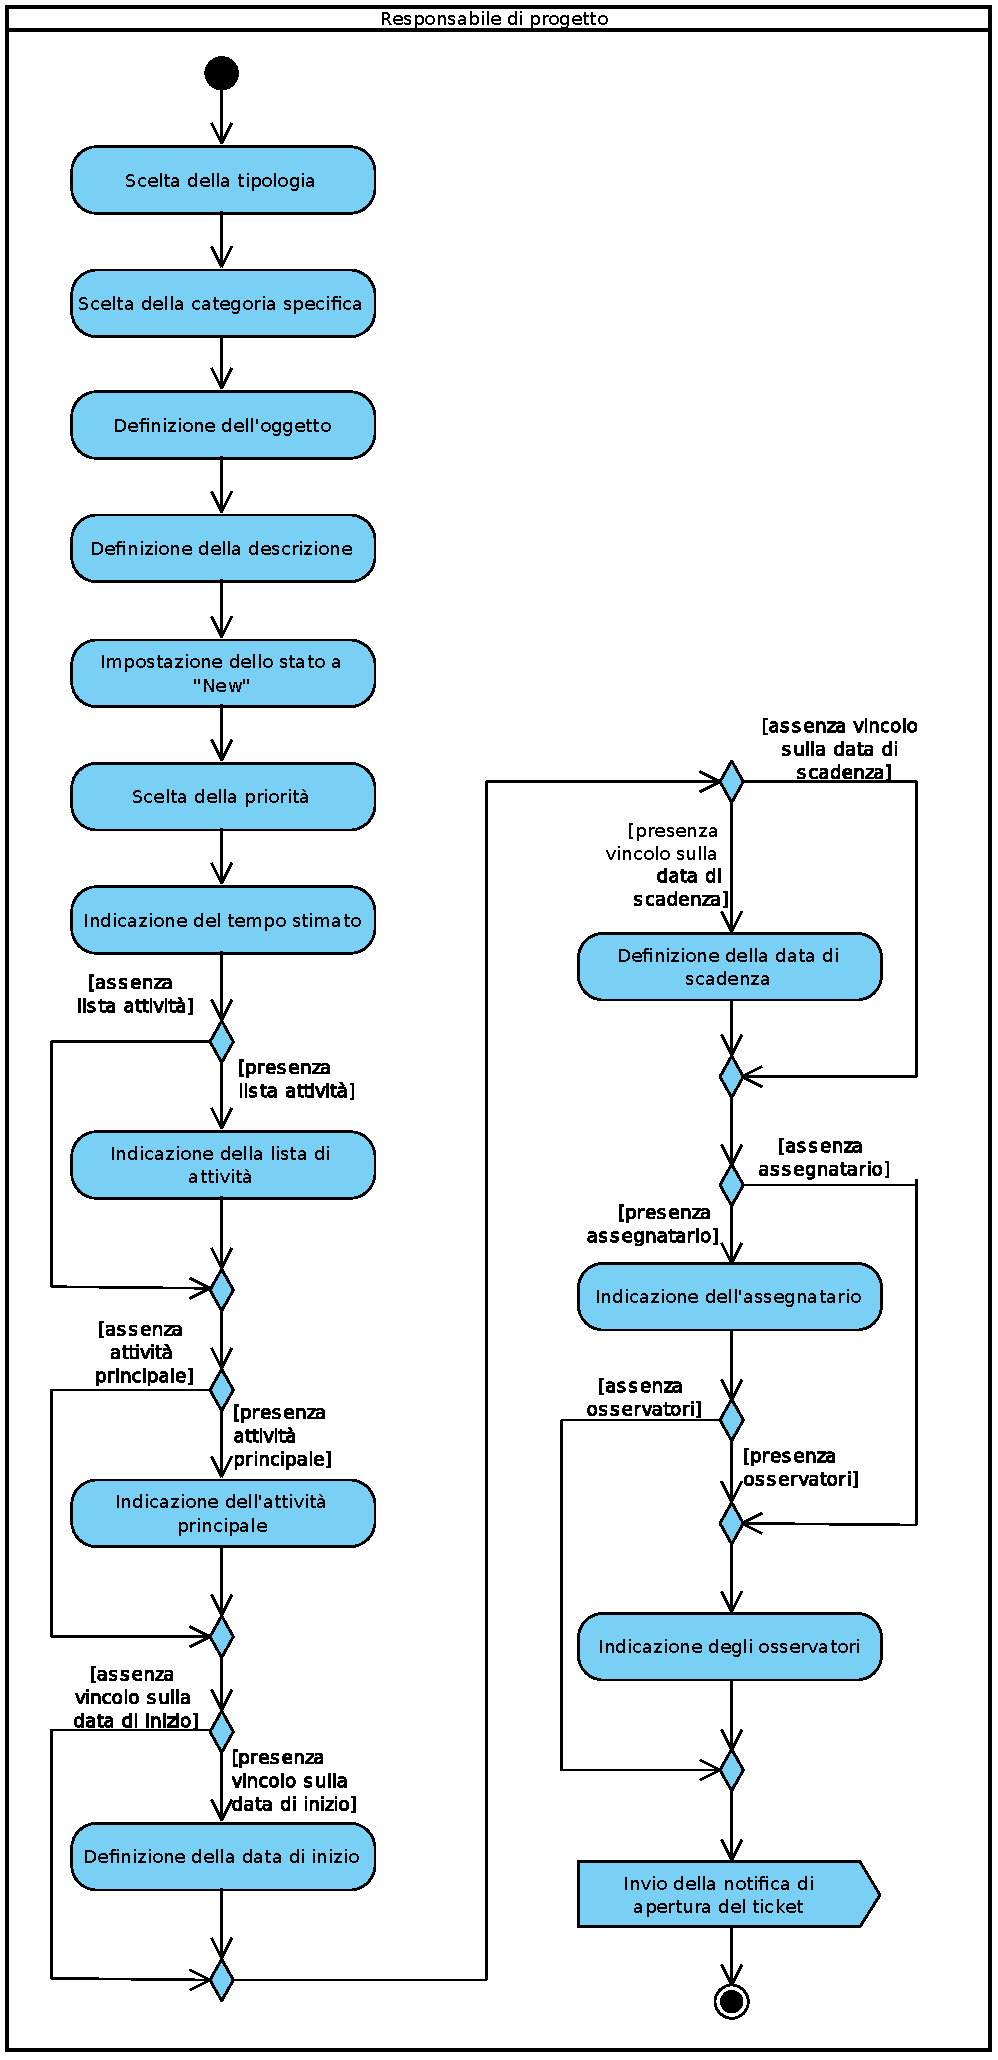
\includegraphics[width=10cm]{../immagini/aperturaTicket.pdf}
\caption{Diagramma di attività - apertura di un ticket}
\label{fig:aperturaTicket}
\end{figure}
\subsubsubsection{Rigetto di un ticket}
La procedura di rigetto di un ticket da parte del \rRP segue il diagramma di attività riportato in \customRef{fig:rigetto_chiusuraTicket}{figura}.
Il \rRP:
\begin{enumerate}
\item Riceve la notifica di un ticket con stato ``Approved'';
\item Effettua una rapida ricerca per trovare eventuali anomalie non catturate dal \rV, che dà esito positivo;
\item Crea una lista con le anomalie trovate;
\item Imposta lo stato del ticket a ``Rejected'' e lo commenta con il link alla lista delle anomalie;
\item Apre i ticket per la correzione delle anomalie;
\item Apre un ticket per la verifica della correzione delle anomalie.
\end{enumerate}
\subsubsubsection{Chiusura di ticket}
La procedura di chiusura di ticket segue il diagramma di attività riportato in \customRef{fig:rigetto_chiusuraTicket}{figura}.
L'attività di chiusura di ticket è delegata al \rRP, che:
\begin{enumerate}
\item Riceve la notifica di un ticket con stato ``Approved'';
\item Effettua una rapida ricerca per trovare eventuali anomalie non catturate dal \rV, che dà esito negativo.
\end{enumerate}
oppure:
\begin{enumerate}
\item Riceve la notifica di un ticket con stato ``Rejected'', accompagnata dalla lista delle anomalie trovate dal verificatore;
\item Apre i ticket per la correzione delle anomalie;
\item Apre un ticket per la verifica della correzione delle anomalie.
\end{enumerate}
Infine, il \rRP imposta lo stato del ticket a ``Closed''.
\begin{figure}[H]
\centering
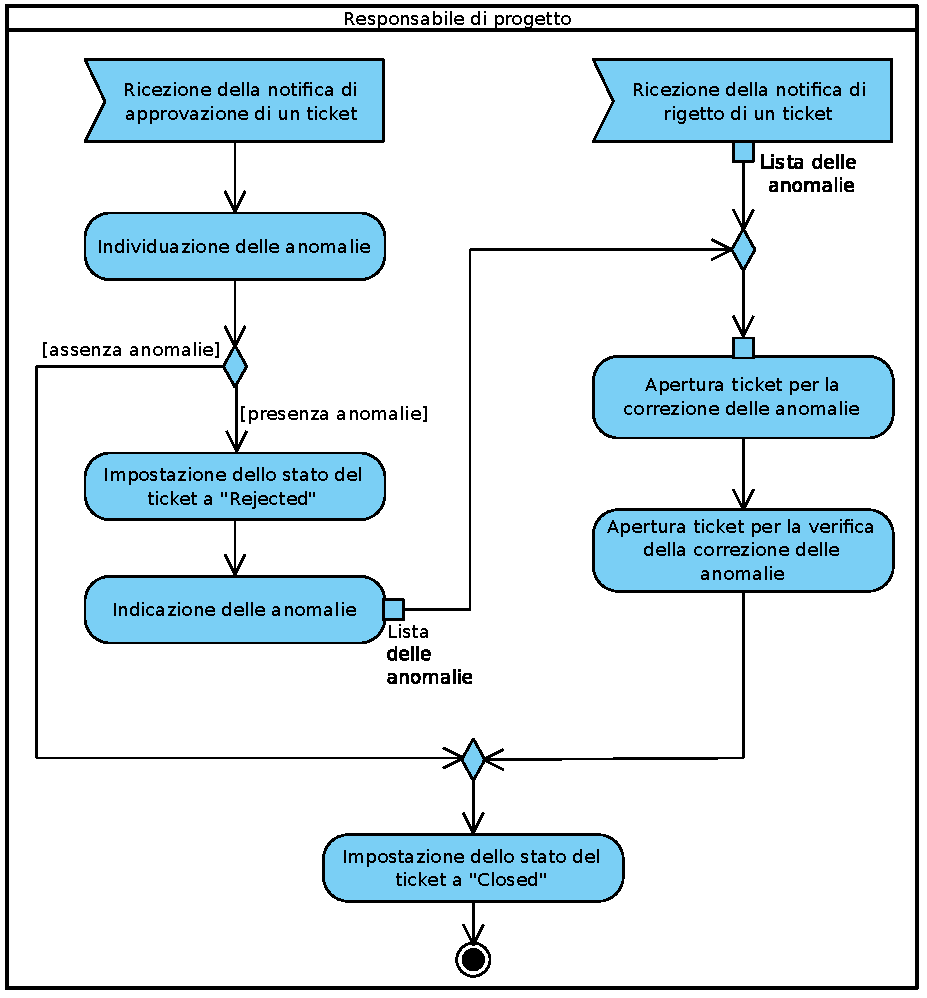
\includegraphics[width=9cm]{../immagini/rigetto_chiusuraTicket.pdf}
\caption{Diagramma di attività - rigetto/chiusura di ticket}
\label{fig:rigetto_chiusuraTicket}
\end{figure}
\subsubsubsection{Rilevazione dei rischi}\label{procRilevazRischi}
In ciascuna fase del \gloxy{progetto}, il \rRP avrà il compito di individuare i rischi indicati nel \PP.
Nel caso si verifichino problematiche non previste, il \rRP dovrà includerle nell’analisi dei rischi.
Complessivamente la procedura di rilevazione dei rischi prevede i seguenti passi:
\begin{enumerate}
\item Rilevazione dei problemi non calcolati;
\item Analisi e classificazione dei nuovi rischi individuati;
\item Pianificazione di controllo dei nuovi rischi individuati;
\item Definizione di contromisure per i nuovi rischi individuati.
\end{enumerate}
\begin{figure}[H]
\centering
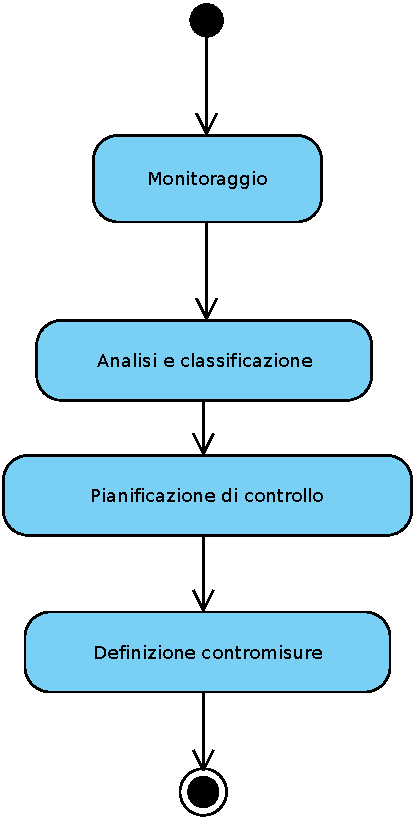
\includegraphics[width=5cm]{../immagini/analisiRischi.pdf}
\caption{Diagramma di attività - rilevazione dei rischi}
\label{fig:rilevazione rischi}
\end{figure}

\subsubsection{Norme}
\subsubsubsection{Template}
Per agevolare e uniformare la redazione dei documenti è stato creato un \gloxy{template} \LaTeX~ contenente tutte le impostazioni stilistiche e i comandi citati in questo documento.\\
Il \gloxy{template} è disponibile nel \gloxy{repository} \texttt{\pragmaDocs} all'interno della cartella \texttt{\nogloxy{template}}.
\subsubsubsection{Norme tipografiche}\label{normeTipografiche}
Questa sezione racchiude le convenzioni adottate da \gruppo per scrivere i documenti in modo uniforme.
\subsubsubsubsection{Norme riguardo nomi}\label{norNome}
Ogniqualvolta si debbano elencare i nomi completi dei componenti del gruppo, tale elenco dovrà essere ordinato lessicograficamente per cognome, e deve sempre essere indicato prima il nome e poi il cognome.
\subsubsubsubsection{Stile del testo}
\begin{itemize}
\item \textbf{Corsivo:} deve essere usato quando ci si riferisce al nome di un documento o a un ruolo, quando si scrivono delle citazioni o abbreviazioni e in tutti gli altri casi in cui si ritiene sia utile mettere in rilievo del testo;
\item \textbf{Grassetto:} può essere usato per evidenziare delle parole chiave oppure per evidenziare il concetto sviluppato da una voce in un elenco puntato;
\item \textbf{\gloxy{Monospace}:} deve essere utilizzato quando si riportano parti di codice, comandi o \gloxy{percorsi} di file;
\item \textbf{Maiuscolo:} l'utilizzo del maiuscolo è riservato solamente per le macro;
\item \textbf{\LaTeX:} per riferirsi a \LaTeX~ è obbligatorio usare l'apposito comando $\backslash$LaTeX.
\end{itemize}
\subsubsubsubsection{Punteggiatura}
\begin{itemize}
\item \textbf{Punteggiatura:} un carattere di punteggiatura non deve mai essere preceduto da un carattere di spaziatura;
\item \textbf{Parentesi:} il testo racchiuso tra parentesi non deve mai iniziare o terminare con un carattere di spaziatura o di punteggiatura, inoltre all'interno del testo racchiuso tra parentesi non deve esserci un altro gruppo di parentesi;
\item \textbf{Lettere maiuscole:} le lettere maiuscole vanno usate per indicare il nome del \gloxy{team}, del \gloxy{progetto}, dei documenti, dei ruoli, delle fasi di lavoro, nelle parole \gloxy{Proponente} e \gloxy{Committente}, all'inizio di un punto di un elenco puntato e in tutte le occasioni in cui ne è previsto l'uso dalla lingua italiana;
\item \textbf{Ritorno a capo:} la decisione riguardo l'uso del ritorno a capo è lasciata a chi scrive il documento, questo perché l'andare a capo dipende dal contesto.
\end{itemize}
Queste convenzioni possono essere trascurate solamente quando si inserisce del codice sorgente all'interno del documento.
\subsubsubsubsection{Composizione del testo}
\begin{itemize}
\item \textbf{Elenchi puntati:} ogni punto dell'elenco deve terminare con un punto e virgola, fatta eccezione per l'ultimo elemento che deve terminare con un punto. La prima parola deve iniziare con una lettera maiuscola, salvo casi particolari in cui è richiesto l'uso della lettera minuscola (es: nome di un file);
\item \textbf{Note a pié pagina:} ogni nota deve cominciare con l'iniziale della prima parola maiuscola e non deve essere preceduta da alcun carattere di spaziatura. Ogni nota deve inoltre terminare con un punto;
\item \textbf{Sigle:} l'uso delle sigle è consentito solamente nei casi in cui sia necessario risparmiare spazio come per esempio nelle tabelle o diagrammi. Le sigle che si prevedono di utilizzare sono:
\begin{itemize}
\item \textbf{AdR:} \AR;
\item \textbf{GL:} \G;
\item \textbf{NdP:} \NP;
\item \textbf{PdP:} \PP;
\item \textbf{PdQ:} \PQ;
\item \textbf{SdF:} \SF;
\item \textbf{ST:} \ST;
\item \textbf{RR:} \RR;
\item \textbf{RP:} \RP;
\item \textbf{RQ:} \RQ;
\item \textbf{RA:} \RA;
\item \textbf{Re:} \rRP;
\item \textbf{Am:} \rAP;
\item \textbf{An:} \rA;
\item \textbf{Pt:} \rP;
\item \textbf{Ve:} \rV;
\item \textbf{Pr:} \rp.
\end{itemize}
\end{itemize}
\subsubsubsubsection{Formati ricorrenti}
\begin{itemize}
\item \textbf{\gloxy{Percorsi}:} per gli indirizzi email e \gloxy{web} deve essere utilizzato il comando $\backslash$url, mentre per gli indirizzi relativi va usato il comando \LaTeX~$\backslash$texttt che usa il formato \gloxy{monospace};
\item \textbf{Date:} le date dovranno seguire il formato
\begin{center}
AAAA-MM-GG
\end{center}
dove:
\begin{itemize}
\item[-] AAAA: rappresenta l'anno scritto utilizzando 4 cifre;
\item[-] MM: rappresenta il mese scritto utilizzando sempre 2 cifre;
\item[-] GG: rappresenta il giorni scritto utilizzando sempre 2 cifre.
\end{itemize}
\item \textbf{Numeri:} i numeri saranno formattati secondo lo standard [SI/ISO 31-0];
\item \textbf{Nome dei file:} per riferirsi ad un file usandone solo il nome è necessario utilizzare il formato \gloxy{monospace};
\item \textbf{Nome dei documenti:} per garantire la scrittura uniforme del nome dei documenti sono stati inseriti dei comandi distinti dalle iniziali maiuscole del nome del documento, ad esempio $\backslash$NP che stampa \NP. \\
Nel caso sia necessario fare riferimento alla versione più aggiornata del documento sono stati predisposti dei comandi \LaTeX~$\backslash$nomeDelDocumento che stampano in modo corretto il nome del documento e l'ultima versione approvata, ad esempio \normeDiProgetto;
\item \textbf{Ruoli di \gloxy{progetto}:} per garantire la scrittura uniforme dei ruoli di \gloxy{progetto} sono stati inseriti dei comandi distinti dalle iniziali maiuscole del nome del ruolo e che hanno come prefisso una ``r'', ad esempio $\backslash$rRP stampo \rRP;
\item \textbf{Revisioni:} per garantire la scrittura uniforme delle revisioni sono stati inseriti dei comandi caratterizzati dalle iniziali maiuscole dei nomi delle revisioni, ad esempio $\backslash$RR stampa \RR;
\item \textbf{Fasi del \gloxy{progetto}:} per garantire la scrittura uniforme del nome delle fasi sono stati inseriti dei comandi caratterizzati dalle iniziali maiuscole del nome delle fasi preceduti da un ``f'', ad esempio $\backslash$fAD stampa \fAD;
\item \textbf{Nomi dei componenti:} per riferirsi ai componenti del \gloxy{team} sono state definite le seguenti macro:
\begin{itemize}
\item[-] \textbf{$\backslash$ao}: \ao;
\item[-] \textbf{$\backslash$fv}: \fv;
\item[-] \textbf{$\backslash$sm}: \sm;
\item[-] \textbf{$\backslash$mb}: \mb;
\item[-] \textbf{$\backslash$dm}: \dm;
\item[-] \textbf{$\backslash$gmi}: \gmi;
\item[-] \textbf{$\backslash$gma}: \gma.
\end{itemize}
\item \textbf{Nome del gruppo:} ci si riferirà al gruppo solamente con il nome \gruppo , per scrivere in modo corretto il nome è stata definita la macro $\backslash$gruppo;
\item \textbf{Nome del \gloxy{Proponente}:} ci si riferirà al \gloxy{Proponente} come ``\proponente'' o con ``Proponente''. Per la corretta scrittura è stata definita la macro $\backslash$proponente;
\item \textbf{Nome del referente del \gloxy{Proponente}:} ci si riferirà al referente del \gloxy{Proponente} come ``\referenteProponente'' o con ``Referente \proponente''. Per la corretta scrittura è stata definita la macro $\backslash$referenteProponente;
\item \textbf{Nome del \gloxy{Committente}:} ci si riferirà al \gloxy{Committente} come ``\committente'' o con ``Committente''. Per la corretta scrittura è stata definita la macro $\backslash$committente;
\item \textbf{Nome del \gloxy{progetto}:} ci si riferirà al \gloxy{progetto} solo come ``\progetto'' . Per la corretta scrittura è stata definita la macro $\backslash$progetto.
\end{itemize}
Un file con i comandi appena descritti è reperibile al seguente link: \\
\url{https://docs.google.com/document/d/1dRy2r-Ewp7Ye8iP-YKJz3T5XkkRIbCOZEPJ-aZocWK4/edit}
\subsubsubsection{Componenti grafiche}
\subsubsubsubsection{Tabelle}
Ad ogni tabella presente all'interno dei documenti deve essere associata una didascalia e un numero identificativo incrementale al fine di renderla tracciabile all'interno del documento.
\subsubsubsubsection{Immagini}
Il formato preferibile per le immagini è \gloxy{PDF}, ma qualora non fosse disponibile è desiderabile l'uso de formato \gloxy{PNG}.
\subsubsubsection{Struttura dei documenti}
\subsubsubsubsection{Frontespizio}
La prima pagina di ogni documento contiene, nell'ordine, le seguenti informazioni:
\begin{itemize}
\item Nome del \gloxy{progetto};
\item Logo e nome del gruppo;
\item Titolo del documento;
\item Versione del documento
\item Nome e cognome dei redattori del documento;
\item Nome e cognome dei \rVs del documento;
\item Nome e cognome del \rRP, che dovrà approvare il documento;
\item Uso del documento;
\item Lista di distribuzione del documento;
\item Descrizione del documento;
\item Anno accademico;
\item Mail del \gloxy{team}.
\end{itemize}
\subsubsubsubsection{Diario delle modifiche}\label{diarioModifiche}
La seconda pagina di ogni documento contiene il diario delle modifiche, cioè una tabella contenente le seguenti informazioni:
\begin{itemize}
\item Data della modifica;
\item Descrizione delle modifiche effettuate; specificandone, quando possibile, le sezioni interessate, e segnalando eventuali riferimenti a sezioni di documenti esterni coinvolti (per riferirsi a decisioni prese in verbali ufficiali si veda la \customRef{verbaliUfficiali}{sezione});
\item Nome e cognome dell'autore;
\item Ruolo ricoperto all'interno del gruppo dall'autore della modifica;
\item Versione del documento dopo la modifica.
\end{itemize}
Le righe della tabella saranno ordinate per data decrescente, in modo che la prima riga della tabella corrisponda all'ultima modifica effettuata.
\subsubsubsubsection{Indici}
Dopo il diario delle modifiche è presente l'indice delle sezioni, e a seguire, solo nel caso siano presenti figure o tabelle, gli indici delle figure e delle tabelle.
\subsubsubsubsection{Struttura generale di una pagina}
L'intestazione di ogni pagina contiene:
\begin{itemize}
\item Il nome del gruppo;
\item La sezione corrente del documento.
\end{itemize}
Il pié di pagina contiene:
\begin{itemize}
\item Il nome del documento;
\item Il numero di pagina corrente espresso nella forma \textit{Pagina: X / Y}, dove X è il numero di pagina corrente e Y è il numero di pagine totali.
\end{itemize}
\subsubsubsection{Tipi di documenti}
\subsubsubsubsection{Documenti interni}
Rappresentano documenti redatti per un utilizzo interno a \gruppo, che non devono essere distribuiti all'esterno e
che non necessitano di \gloxy{versionamento}. Questa tipologia di documentazione verrà archiviata su \gloxy{Google Drive}.
A questa categoria di documenti appartengono le bozze di documento e i verbali interni informali.
\subsubsubsubsubsection{Verbali interni informali}
Un verbale interno informale è un documento che descrive gli argomenti discussi durante una riunione tra soli membri del \gloxy{team}, che dovrà restare a loro esclusiva disposizione. Verrà redatto da un membro del \gloxy{team}, condiviso mediante \gloxy{Google Drive}, e inviato a tutti i suoi componenti tramite posta elettronica.
\subsubsubsubsubsection{Bozze di documenti ufficiali}
Per velocizzare la stesura dei documenti informali è possibile iniziare a scrivere un bozza,
in  modo che anche i membri del gruppo che non sono familiari con \LaTeX~ possano iniziare a produrre materiale fin da subito.
Quando viene creata una bozza è necessario comunicarlo in \gloxy{mailing list} usando come oggetto:
\begin{center}
\texttt{[Bozza] Nome del documento}
\end{center}
In ogni caso è necessario che la bozza sia promossa a documento informale il prima possibile.
\subsubsubsubsection{Documenti ufficiali}
\subsubsubsubsubsection{Verbali ufficiali}\label{verbaliUfficiali}
Un verbale ufficiale è un documento che descrive gli argomenti discussi durante una riunione con il \gloxy{Proponente} (verbale interno) o con il \gloxy{Committente} (verbale esterno), ed ha quindi valore normativo.
\\Ogni sezione del documento dovrà essere dedicata ad un particolare problema trattato all'incontro, che dovrà essere presentato e ne dovrà essere descritta la relativa decisione presa con il \gloxy{Committente}.
\\Il documento dovrà essere consultabile dal \gloxy{team} e dalle parti esterne, quindi verrà allegato ad un messaggio di risposta alla mail di convocazione della riunione esterna e inviato alla \gloxy{mailing list} del \gloxy{team}.
Per agevolarne l'identificazione, i verbali interni verranno denominati con un codice univoco \emph{TN}, dove:
\begin{itemize}
\item \emph{T} rappresenta il tipo del verbale: \emph{E}, per i verbali esterni relativi a riunioni tenute con il \gloxy{Committente}, e \emph{I}, per i verbali interni relativi a riunioni con il \gloxy{Proponente};
\item \emph{N} è un numero intero che parte da \emph{1} e viene incrementato per ogni nuovo verbale di tipo \emph{T} di verbale.
\end{itemize}
Per riferirsi ad una precisa decisione di un verbale ufficiale\footnote{I verbali dovranno comparire anche tra i riferimenti normativi del documento.}, è sufficiente indicare il codice univoco del verbale seguito da un trattino e dal numero della decisione interessata. Per fare ciò si deve utilizzare la notazione \emph{TN-D}, dove \emph{TN} è il codice dell’\emph{N}-esimo verbale ufficiale e \emph{D} è la \emph{D}-esima decisione.
\subsubsubsubsubsection{Documenti informali}
Un documento è ritenuto informale finché non viene approvato dal \rRP.
Appartengono a questa categoria tutti i documenti che dovranno essere consegnati al \gloxy{Committente} o al \gloxy{Proponente},
questi documenti sono memorizzati nel \gloxy{repository} \texttt{\pragmaDocs} e devono attenersi alle \NP.
\subsubsubsubsubsection{Documenti formali}
Un documento diventa formale quando viene approvato dal \rRP.
Per raggiungere questo stato è necessario che il documento sia conforme alle \NP e che abbia seguito il \gloxy{percorso} di verifica e validazione in esse descritto.
\subsubsubsubsubsection{\G}
Il \G conterrà le \emph{parole} dei documenti che possono far parte del contesto dell'applicazione e i \emph{termini} che possono generare ambiguità d'interpretazione. Tali termini saranno disposti in ordine alfabetico ed ognuno di essi avrà una definizione, che dovrà essere sintetica e precisa, per non creare equivoci o ambiguità.
Ogni membro del \gloxy{team} è invitato a inserire nel \G le parole da esso individuate, delle quali non esista ancora una definizione. L'inserimento dei termini nel \G avverrà parallelamente alla stesura dei documenti sfruttando le funzionalità offerte da \pragmadb.
%I termini verranno inseriti nel \G parallelamente alla stesura degli altri documenti, in modo da evitare errori umani.\\
\subsubsubsection{Versionamento}\label{versionamento}
L'avanzamento di versione da parte dei documenti sarà espresso nella seguente forma:
\begin{center}
vX.Y.Z
\end{center}
dove:
\begin{itemize}
\item \textbf{X}: indica il numero di uscite formali del documento e viene incrementato in corrispondenza con l'ultima approvazione del \rRP prima del rilascio. L'incremento di \textbf{X} comporta l'azzeramento sia di \textbf{Y} che di \textbf{Z};
\item \textbf{Y}: indica il numero di modifiche e correzioni effettuate al documento. L'incremento \textbf{Y} comporta l'azzeramento di \textbf{Z};
\item \textbf{\textbf{Z}}: quando vale\begin{itemize}[label=\ding{212}]
\item 0: indica che le ultime modifiche (successive all'ultima verifica) non sono state verificate;
\item 1: indica che le ultime modifiche (successive all'ultima verifica) sono state verificate;
\item 2: indica che l'ultima verifica è stata approvata.
\end{itemize}
\end{itemize}
Quando si fa riferimento al contenuto di una specifica versione di un documento, ne è richiesta la sua precisazione usando la seguente sintassi:
\begin{center}
\textit{NomeDocumento vX.Y.Z}
\end{center}
Quando saranno creati i file, il loro nome dovrà seguire lo schema:
\begin{center}
\texttt{nomeDocumento\_vX.Y.Z.pdf}
\end{center}

\subsubsection{Strumenti}
\subsubsubsection{\pragmadb}\label{PragmaDB}
\pragmadb è un'applicazione \gloxy{web} sviluppata dal \gloxy{team} per la gestione di casi d'uso, attori, fonti, requisiti e termini del \G. Il suo scopo è velocizzare e automatizzare la gestione dei dati, e semplificare i tracciamenti. Ogni membro del \gloxy{team} può accedere all'applicazione via \gloxy{browser} previa autenticazione, inoltre, più persone possono lavorare simultaneamente sugli stessi dati poiché è stata gestita la concorrenza. L'applicazione si occupa di mantenere ordinata la gerarchia dei requisiti e degli UC in modo automatico durante tutto il suo ciclo di vita (creazione, modifica, eliminazione).\\
Vengono eseguiti diversi controlli su ciascun campo dati, e tale approccio garantisce \gloxy{fault-tolerance} del sistema nei confronti di qualsiasi input possibile. I membri del gruppo possono visualizzare, inserire, modificare ed eliminare elementi in modo semplice. \pragmadb consente di esportare l'elenco degli attori, delle fonti, del \G, dei casi d'uso, dei requisiti e delle loro relazioni come codice \LaTeX, quindi facilmente inseribile all'interno dei documenti durante la stesura. Infine consente di visualizzare, attraverso un menù laterale, l'insieme dei link utili relativi al gruppo (link al \gloxy{repository}, link al foglio dei comandi \LaTeX, link a Redmine, link alla \gloxy{mailing list} Yahoo).
\subsubsubsubsection{Attori}
La sezione degli attori è pensata per mantenere traccia di tutti gli attori del sistema.
Un attore è caratterizzato da un nome identificativo e da una descrizione. \`{E} possibile inserire, modificare o eliminare attori, ed esportare in \LaTeX\ una tabella contenente tutte le informazioni su di essi.
Cliccando sul nome di un attore è possibile vederne il dettaglio dello stesso, che mostra in particolare, una lista dei casi d'uso correlati, per facilitarne il processo di verifica.
\`E consentita l'eliminazione di un attore solamente se non esiste alcun caso d'uso ad essa riferito.
\subsubsubsubsection{Fonti}
La sezione delle fonti è pensata per mantenere traccia di tutte le fonti (capitolati, verbali, ecc\dots) che hanno determinato l'individuazione di un requisito.
Una fonte è caratterizzata da un identificativo, un nome e una descrizione. \`{E} possibile inserire, modificare o eliminare fonti, ed esportare in \LaTeX\ una tabella contenente tutte le informazioni su di esse.
Cliccando sull'identificativo di una fonte è possibile vederne il dettaglio dello stesso, che mostra in particolare, una lista dei requisiti correlati, per facilitarne il processo di verifica.
\`E consentita l'eliminazione di una fonte solamente se non esiste alcun requisito derivato da essa.
\subsubsubsubsection{Requisiti}
La sezione dei requisiti è pensata per mantenere traccia di tutti i requisiti individuati.
Un requisito è caratterizzato da un identificativo, un tipo (funzionale, di vincolo, di qualità, prestazionale), un livello di importanza (obbligatorio, desiderabile, facoltativo),
un requisito padre (se non è radice), uno stato (accettato/non accettato + soddisfatto/non soddisfatto + implementato/non implementato), una o più fonti di riferimento e una descrizione. \`{E} possibile inserire, modificare o eliminare requisiti, ed esportare in \LaTeX\ una tabella contenente tutte le informazioni su di essi.
Cliccando sull'identificativo di un requisito è possibile vederne il dettaglio dello stesso, che mostra in particolare, una lista dei requisiti figli e dei casi d'uso correlati, per facilitarne il processo di verifica.
\`E inoltre presente una funzionalità che permette di vedere quali requisiti non sono correlati ad alcun caso d'uso.
\subsubsubsubsection{Casi d'uso}
La sezione dei casi d'uso è pensata per mantenere traccia di tutti i casi d'uso individuati dagli \rAs.
Un caso d'uso è caratterizzato da un identificativo, un nome, un diagramma, una o più precondizioni, una o più postcondizioni, un caso d'uso padre (se non è radice), uno scenario principale, una o più inclusioni (facoltativo), una o più estensioni (facoltativo), uno o più scenari alternativi (facoltativo) e una descrizione. \`{E} possibile inserire, modificare o eliminare casi d'uso, ed esportare in \LaTeX\ una tabella contenente tutte le informazioni su di essi.
Cliccando sull'identificativo di un caso d'uso è possibile vederne il dettaglio dello stesso, che mostra in particolare, una lista dei casi d'uso figli e dei requisiti correlati, per facilitarne il processo di verifica.
\`E inoltre presente una funzionalità che permette di vedere quali casi d'uso non sono correlati ad alcun requisito.
\subsubsubsubsection{\G}
Nell'area dedicata alla gestione del \G è possibile inserire, modificare o eliminare termini, ed esportare in \LaTeX\ l’intero \G sotto forma di lista di \texttt{newglossaryentry}, macro fornita dal package \texttt{glossaries} di \LaTeX.
Una voce di \G è caratterizzata da un \emph{identificativo}, un \emph{nome} singolare che verrà mostrato nel \G, una descrizione, un \emph{plurale} (facoltativo) per indicare la sua forma plurale, una forma \emph{estesa} (facoltativo) per indicare la forma singolare (più rara) che il termine può assumere alla sua prima occorrenza all'interno dei documenti, una forma \emph{estesa plurale} (facoltativo) per indicare la forma plurale (più rara) che il termine può assumere alla sua prima occorrenza nei documenti e un \emph{sinonimo} (facoltativo).
\subsubsubsubsection{Package e Classi}\label{pdbPackageClassi}
Per ciascun componente (package o classe) è possibile specificare:
\begin{itemize}
\item Un diagramma \gloxy{UML};
\item Una descrizione testuale del componente;
\item Una descrizione del contesto d'utilizzo;
\item Le relazioni con gli altri componenti;
\item I requisiti che il componente va a soddisfare.
\end{itemize}
Per le classi è inoltre possibile specificare gli attributi e i metodi che le caratterizzano e l'eventuale gerarchia di classi a cui appartengono. Alcuni screenshot esemplificativi di queste funzionalità sono stati inseriti nell'\customRef{screenPDB}{appendice}.
\subsubsubsubsection{Test}\label{pdbTest}
In questa sezione è possibile inserire i test definiti dai \rPs{}. Ogni test è caratterizzato da un tipo e una descrizione.
I tipi di test sono: validazione, sistema, integrazione oppure unità; e in base a tale tipo, un test può essere associato a un requisito, a un componente oppure a un metodo di una classe.
%L'associazione tra il test e l'elemento è \emph{1 a 1}: ad un test può essere associato un solo elemento e viceversa.\\
Ogni test è caratterizzato da un id univoco, calcolato automaticamente da \pragmadb e da una serie di parametri che specificano se il test è stato implementato, eseguito e superato.
\subsubsubsubsection{Tracciamento} \label{pragmadbTracciamento}
\pragmadb consente di esportare direttamente in \LaTeX\ molte parti dei documenti
del \gloxy{progetto}, automatizzandone il processo di stesura. Grazie ad uno script
appositamente creato è possibile in ogni momento scaricare tutti i file \LaTeX, inserendoli
nelle cartelle dei rispettivi documenti.
\pragmadb consente il tracciamento delle seguenti coppie di elementi:
\begin{itemize}
\item Requisiti - Fonti;
\item Fonti - Requisiti;
\item Componenti - Requisiti;
\item Requisiti - Componenti;
\item Classi - Requisiti;
\item Requisiti - Classi;
\item Elemento - Test;
\item Test - Elemento.
\end{itemize}
\subsubsubsubsection{Funzionalità di supporto}\label{pdbSupport}
Per semplificare la verifica del tracciamento tra gli elementi memorizzati in \pragmadb, sono state aggiunte funzionalità che permettono di ottenere una lista degli elementi non relazionati con nessun altro elemento. \\
In particolare \pragmadb fornisce la lista di:
\begin{itemize}
\item Requisiti non sono derivati da casi d'uso;
\item Casi d'uso che non generano requisiti;
\item Package che non soddisfano requisiti;
\item Classi che non soddisfano requisiti;
\item Test che non verificano classi o requisiti.
\end{itemize}
\subsubsubsection{WebStorm}
L'ambiente di sviluppo integrato (IDE) utilizzato è \textbf{\gloxy{WebStorm}}. Sono stati testati anche altri \gloxy{IDE}, ma nessuno si è dimostrato all'altezza di \textbf{\gloxy{WebStorm}}. Esso presenta le seguenti funzionalità:
\begin{itemize}
\item Autocompletamento del codice \gloxy{JavaScript}, \gloxy{HTML} 5 e CSS3;
\item Autocompletamento per metodi, funzioni e \gloxy{framework} esterni, utili per il \gloxy{progetto};
\item Debugger \gloxy{JavaScript};
\item Consente di effettuare unit test per \gloxy{JavaScript} mediante il \gloxy{framework} \textbf{\gloxy{Karma}};
\item Compila automaticamente i file \gloxy{Sass} in \gloxy{CSS};
\item Tiene traccia dei cambiamenti effettuati sui file, consentendo di visualizzare lo storico delle modifiche locali e ritornare a versioni precedenti in caso di modifiche o perdite accidentali.
\end{itemize}

\subsection{Processo di verifica}
\subsubsection{Attività}
\subsubsubsection{Analisi dei requisiti} %Si parla di Attività e Task, non ha senso usare il comando per i documenti.
\subsubsubsubsection{Task - Studio di fattibilità}
Alla pubblicazione dei capitolati d'appalto il \rRP avrà il compito di organizzare un adeguato numero di riunioni, affinché i membri del gruppo possano discutere e confrontarsi. A seguito di quanto emerso durante tali riunioni, gli \rAs dovranno procedere con la stesura del documento ``\SF'', che dovrà essere stilato basandosi sui seguenti punti:
\begin{itemize}
\item \textbf{Dominio Tecnologico e Applicativo}: riflessione su tecnologie e tecniche richieste per lo sviluppo del capitolato, dominio tecnologico e conoscenze che il \gloxy{team} già possiede;
\item \textbf{Rapporto Costi/Benefici}: analisi della quantità di requisiti obbligatori e del loro costo in termini di realizzazione in funzione del risultato atteso;
\item \textbf{Individuazione dei Rischi}: comprensione dei punti critici nella realizzazione e individuazione di eventuali rischi.
\end{itemize}
\subsubsubsubsection{Task - Analisi dei requisiti}
Dopo aver concluso lo \SF, gli \rAs dovranno procedere con la stesura del documento ``\AR''.
Lo scopo principale di questa attività è quella di produrre dei requisiti semplici e di facile comprensione, a partire da tutte le informazioni recuperabili. Per automatizzare e velocizzare il più possibile questa attività, è stato creato dal \gloxy{team} il software \pragmadb, in cui andranno inseriti tutti i requisiti.
\subsubsubsection{Progettazione}\label{normeprog}
\subsubsubsubsection{Task - Specifica tecnica}
I \rPs devono definire la struttura ad alto livello dell'architettura del sistema e dei singoli componenti, raccogliendo il tutto nella \ST. Devono, inoltre, essere definiti i test di integrazione tra le varie componenti, che verranno inseriti in appendice al \PQ. \\
I prodotti di questo task saranno:
\begin{itemize}
\item \textbf{Diagrammi \gloxy{UML}:}
\begin{itemize}
\item Diagrammi dei package;
\item Diagrammi delle classi;
\item Diagrammi di sequenza;
\item Diagrammi di attività.
\end{itemize}
\item \textbf{Design pattern:} i \rPs devono fornire una descrizione dei \gloxy{design pattern} adottati nella definizione dell'architettura. Questa descrizione dovrà essere accompagnata da un diagramma \gloxy{UML}, che ne esemplifichi il funzionamento, e dalle motivazioni che hanno portato all'adozione di tale pattern;
\item \textbf{Tracciamento delle componenti:} ogni componente dovrà essere tracciato ed associato ad almeno un requisito. In tal modo sarà possibile avere la certezza che tutti i requisiti accettati siano soddisfatti e che ogni componente presente nell'architettura soddisfi almeno un requisito. Tale tracciamento dovrà essere effettuato tramite \pragmadb, che si occupa di generare in modo automatico le relative tabelle. Maggiori informazioni sono disponibili nella sezione \ref{pragmadbTracciamento};
\item \textbf{Test d'integrazione:} i \rPs devono definire delle strategie di verifica per poter dimostrare la corretta integrazione tra le varie componenti definite.
\end{itemize}
\subsubsubsubsection{Task - Definizione di prodotto}
I Progettisti, a partire dalla \ST, devono produrre la \DP dove viene descritta la progettazione di dettaglio del sistema.
Lo scopo di questo documento è quello di definire dettagliatamente ogni singola unità
di cui è composto il sistema in modo da semplificare l’attività di codifica e allo stesso
tempo di non fornire alcun grado di libertà al Programmatore.
Parallelamente alla progettazione di dettaglio dei componenti software dovranno essere
progettati i relativi test di unità che verranno descritti nel Piano di Qualifica.
I prodotti di questo task saranno:
\begin{itemize}
\item \textbf{Diagrammi \gloxy{UML}:}
\begin{itemize}
\item Diagrammi dei package;
\item Diagrammi delle classi;
\item Diagrammi di sequenza.
\end{itemize}
\item \textbf{Definizione delle classi:} ogni classe precedentemente progettata viene descritta più nel dettaglio, fornendo una descrizione più approfondita dello scopo, delle sue funzionalità e del suo funzionamento. Per ogni classe dovranno essere anche definiti i vari metodi e attributi che la caratterizzano;
\item \textbf{Tracciamento delle classi:} ogni classe deve essere tracciata ed associata ad almeno un requisito, in questo modo è possibile avere la certezza che tutti i requisiti accettati siano soddisfatti e che ogni classe presente nell'architettura soddisfi almeno un requisito. Questo tracciamento dev'essere effettuato tramite \pragmadb, che si occupa di generare in modo automatico le tabelle di tracciamento. Maggiori informazioni sono disponibili nella sezione \ref{pragmadbTracciamento};
\item \textbf{Test di unità:} i \rPs devono definire le strategie di verifica delle varie classi in modo che durante l'attività di codifica sia possibile verificare che la classe si comporti in modo corretto.
\end{itemize}

\subsubsection{Procedure}\label{procedureGestione}
\subsubsubsection{Apertura di un ticket}
La procedura di apertura di un ticket segue il diagramma di attività riportato in \customRef{fig:aperturaTicket}{figura}, e la sua applicazione è delegata al \rRP, che:
\begin{enumerate}
\item Seleziona la tipologia: \emph{task}, \emph{feature}, \emph{\gloxy{bug}} o \emph{step};
\item Seleziona la categoria specifica: \emph{documentazione} o \emph{verifica};
\item Definisce l'\emph{oggetto};
\item Definisce una \emph{descrizione};
\item Imposta lo \emph{stato} a ``\emph{New}'';
\item Seleziona il livello di \emph{priorità}: \emph{low}, \emph{normal}, \emph{high}, \emph{urgent} o \emph{immediate};
\item Indica una \emph{stima del tempo} (in ore) necessario per portarlo a termine;
\item Definisce una \emph{lista di attività} da compiere (facoltativo);
\item Stabilisce l'\emph{attività principale} da eseguire (facoltativo);
\item Definisce la data di \emph{inizio} (facoltativo);
\item Definisce la data di \emph{scadenza} (facoltativo);
\item Sceglie l'\emph{assegnatario} (facoltativo);
\item Indica degli \emph{osservatori} (facoltativo).
\end{enumerate}
L'assegnatario e gli osservatori del ticket ricevono una notifica via mail che li informa della sua apertura.
\\\textbf{N.B.:} qualora non venga scelto alcun assegnatario, dovrà essere indicato almeno un osservatore.
\begin{figure}[H]
\centering
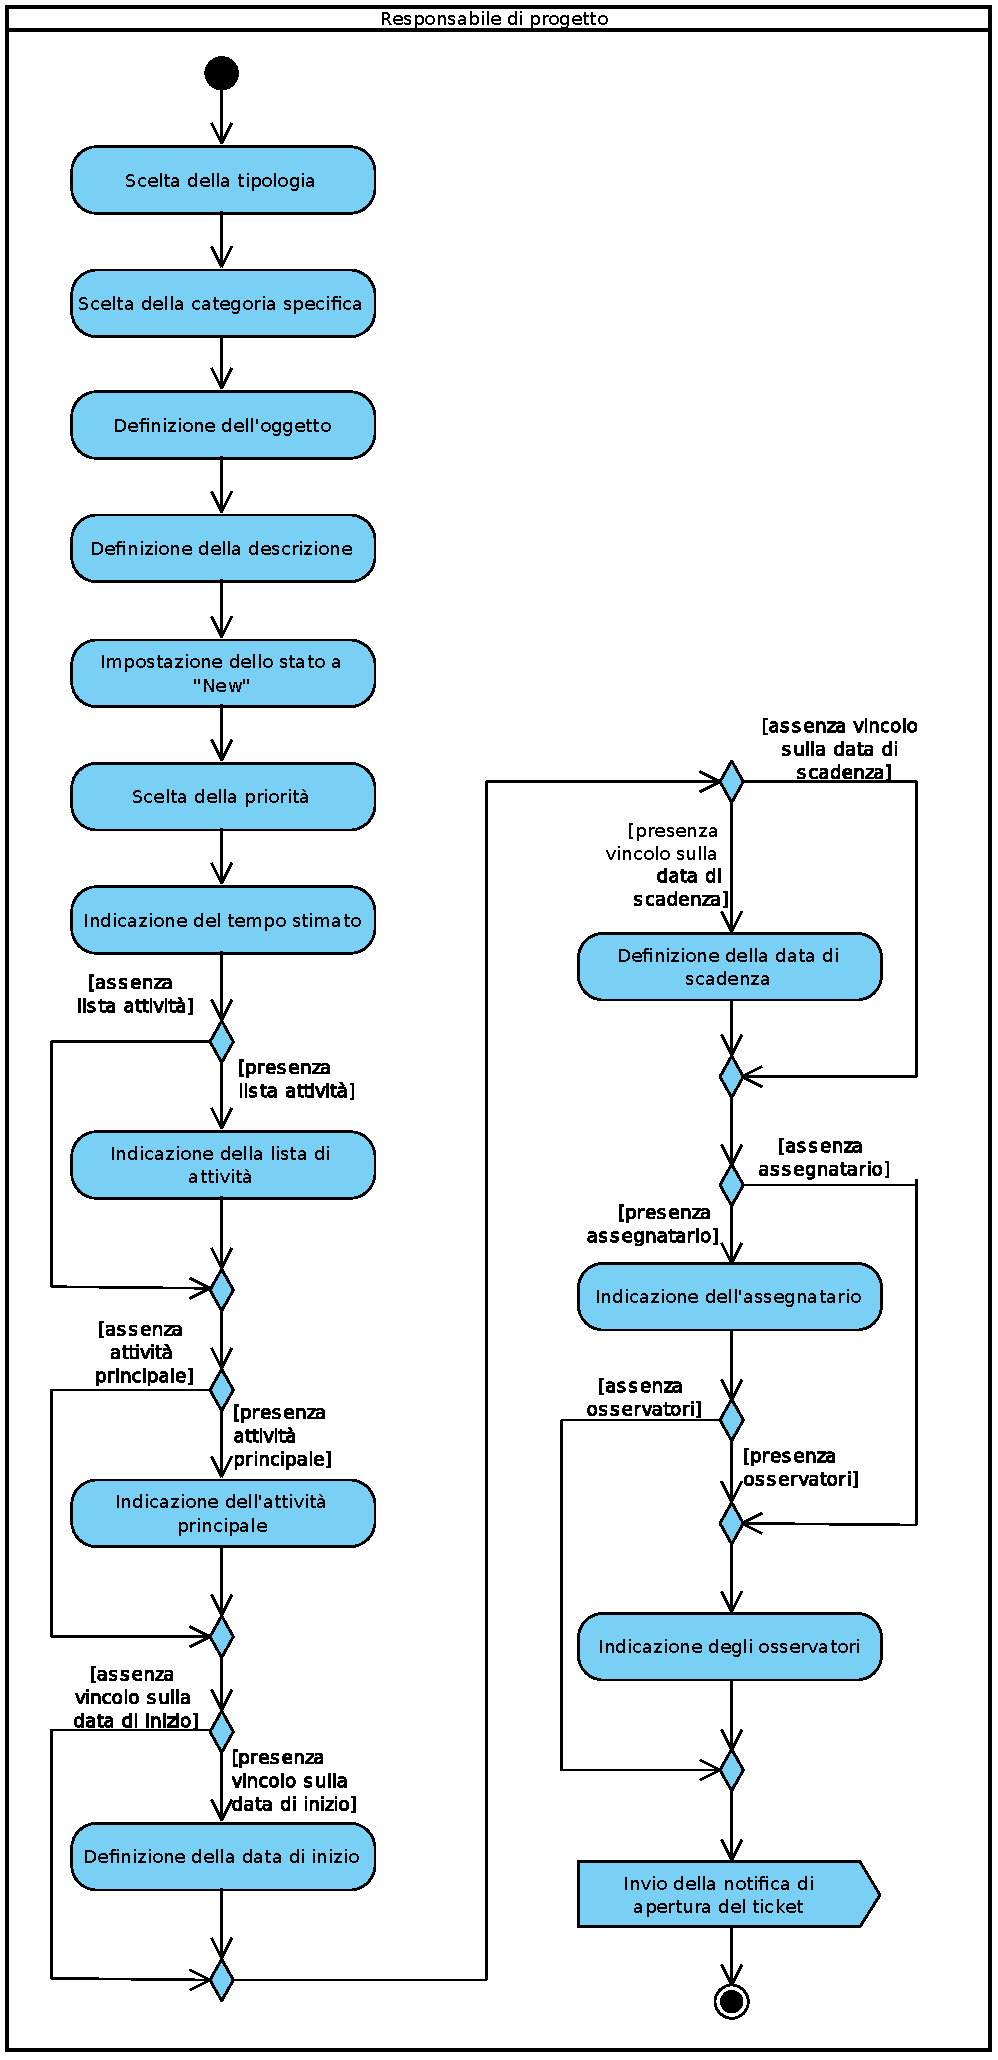
\includegraphics[width=10cm]{../immagini/aperturaTicket.pdf}
\caption{Diagramma di attività - apertura di un ticket}
\label{fig:aperturaTicket}
\end{figure}
\subsubsubsection{Rigetto di un ticket}
La procedura di rigetto di un ticket da parte del \rRP segue il diagramma di attività riportato in \customRef{fig:rigetto_chiusuraTicket}{figura}.
Il \rRP:
\begin{enumerate}
\item Riceve la notifica di un ticket con stato ``Approved'';
\item Effettua una rapida ricerca per trovare eventuali anomalie non catturate dal \rV, che dà esito positivo;
\item Crea una lista con le anomalie trovate;
\item Imposta lo stato del ticket a ``Rejected'' e lo commenta con il link alla lista delle anomalie;
\item Apre i ticket per la correzione delle anomalie;
\item Apre un ticket per la verifica della correzione delle anomalie.
\end{enumerate}
\subsubsubsection{Chiusura di ticket}
La procedura di chiusura di ticket segue il diagramma di attività riportato in \customRef{fig:rigetto_chiusuraTicket}{figura}.
L'attività di chiusura di ticket è delegata al \rRP, che:
\begin{enumerate}
\item Riceve la notifica di un ticket con stato ``Approved'';
\item Effettua una rapida ricerca per trovare eventuali anomalie non catturate dal \rV, che dà esito negativo.
\end{enumerate}
oppure:
\begin{enumerate}
\item Riceve la notifica di un ticket con stato ``Rejected'', accompagnata dalla lista delle anomalie trovate dal verificatore;
\item Apre i ticket per la correzione delle anomalie;
\item Apre un ticket per la verifica della correzione delle anomalie.
\end{enumerate}
Infine, il \rRP imposta lo stato del ticket a ``Closed''.
\begin{figure}[H]
\centering
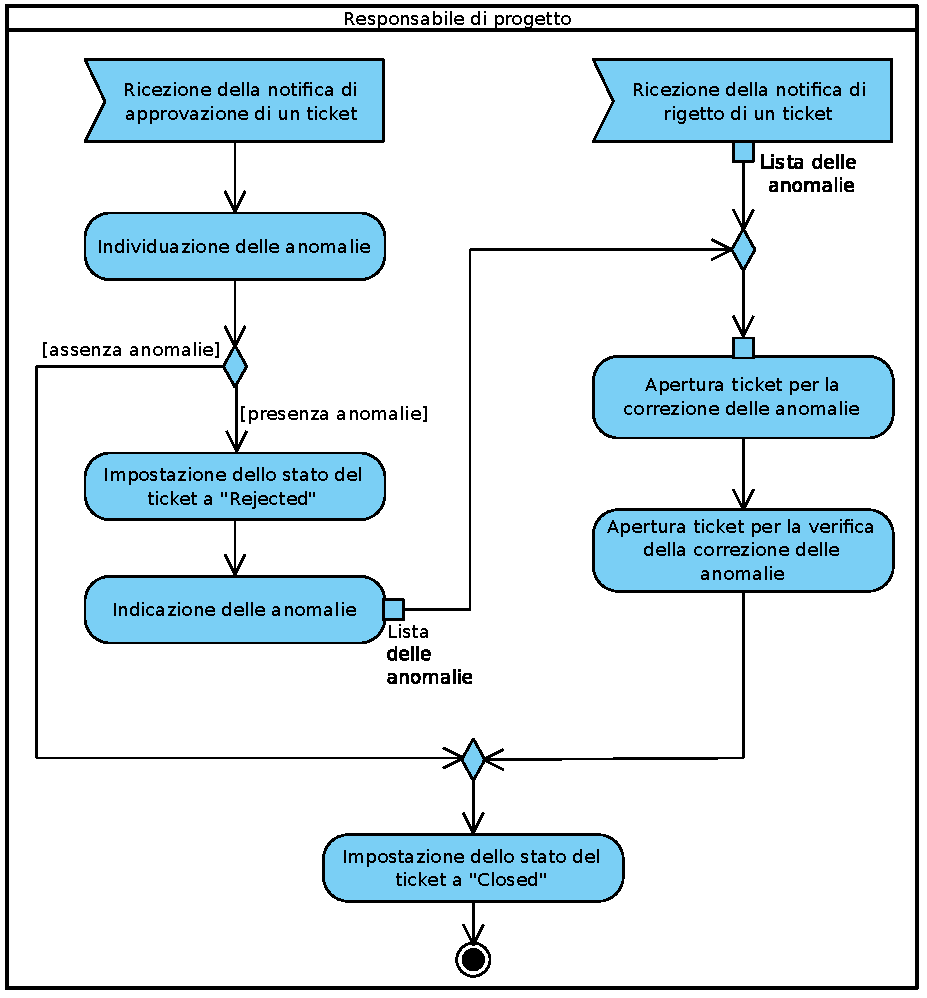
\includegraphics[width=9cm]{../immagini/rigetto_chiusuraTicket.pdf}
\caption{Diagramma di attività - rigetto/chiusura di ticket}
\label{fig:rigetto_chiusuraTicket}
\end{figure}
\subsubsubsection{Rilevazione dei rischi}\label{procRilevazRischi}
In ciascuna fase del \gloxy{progetto}, il \rRP avrà il compito di individuare i rischi indicati nel \PP.
Nel caso si verifichino problematiche non previste, il \rRP dovrà includerle nell’analisi dei rischi.
Complessivamente la procedura di rilevazione dei rischi prevede i seguenti passi:
\begin{enumerate}
\item Rilevazione dei problemi non calcolati;
\item Analisi e classificazione dei nuovi rischi individuati;
\item Pianificazione di controllo dei nuovi rischi individuati;
\item Definizione di contromisure per i nuovi rischi individuati.
\end{enumerate}
\begin{figure}[H]
\centering
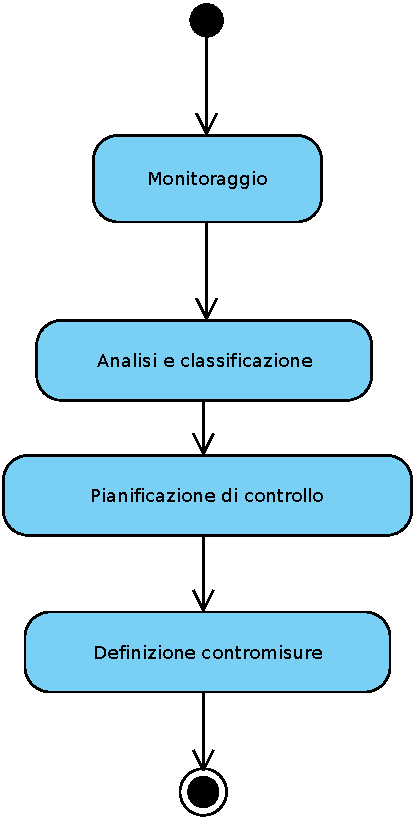
\includegraphics[width=5cm]{../immagini/analisiRischi.pdf}
\caption{Diagramma di attività - rilevazione dei rischi}
\label{fig:rilevazione rischi}
\end{figure}

\subsubsection{Strumenti}
\subsubsubsection{\pragmadb}\label{PragmaDB}
\pragmadb è un'applicazione \gloxy{web} sviluppata dal \gloxy{team} per la gestione di casi d'uso, attori, fonti, requisiti e termini del \G. Il suo scopo è velocizzare e automatizzare la gestione dei dati, e semplificare i tracciamenti. Ogni membro del \gloxy{team} può accedere all'applicazione via \gloxy{browser} previa autenticazione, inoltre, più persone possono lavorare simultaneamente sugli stessi dati poiché è stata gestita la concorrenza. L'applicazione si occupa di mantenere ordinata la gerarchia dei requisiti e degli UC in modo automatico durante tutto il suo ciclo di vita (creazione, modifica, eliminazione).\\
Vengono eseguiti diversi controlli su ciascun campo dati, e tale approccio garantisce \gloxy{fault-tolerance} del sistema nei confronti di qualsiasi input possibile. I membri del gruppo possono visualizzare, inserire, modificare ed eliminare elementi in modo semplice. \pragmadb consente di esportare l'elenco degli attori, delle fonti, del \G, dei casi d'uso, dei requisiti e delle loro relazioni come codice \LaTeX, quindi facilmente inseribile all'interno dei documenti durante la stesura. Infine consente di visualizzare, attraverso un menù laterale, l'insieme dei link utili relativi al gruppo (link al \gloxy{repository}, link al foglio dei comandi \LaTeX, link a Redmine, link alla \gloxy{mailing list} Yahoo).
\subsubsubsubsection{Attori}
La sezione degli attori è pensata per mantenere traccia di tutti gli attori del sistema.
Un attore è caratterizzato da un nome identificativo e da una descrizione. \`{E} possibile inserire, modificare o eliminare attori, ed esportare in \LaTeX\ una tabella contenente tutte le informazioni su di essi.
Cliccando sul nome di un attore è possibile vederne il dettaglio dello stesso, che mostra in particolare, una lista dei casi d'uso correlati, per facilitarne il processo di verifica.
\`E consentita l'eliminazione di un attore solamente se non esiste alcun caso d'uso ad essa riferito.
\subsubsubsubsection{Fonti}
La sezione delle fonti è pensata per mantenere traccia di tutte le fonti (capitolati, verbali, ecc\dots) che hanno determinato l'individuazione di un requisito.
Una fonte è caratterizzata da un identificativo, un nome e una descrizione. \`{E} possibile inserire, modificare o eliminare fonti, ed esportare in \LaTeX\ una tabella contenente tutte le informazioni su di esse.
Cliccando sull'identificativo di una fonte è possibile vederne il dettaglio dello stesso, che mostra in particolare, una lista dei requisiti correlati, per facilitarne il processo di verifica.
\`E consentita l'eliminazione di una fonte solamente se non esiste alcun requisito derivato da essa.
\subsubsubsubsection{Requisiti}
La sezione dei requisiti è pensata per mantenere traccia di tutti i requisiti individuati.
Un requisito è caratterizzato da un identificativo, un tipo (funzionale, di vincolo, di qualità, prestazionale), un livello di importanza (obbligatorio, desiderabile, facoltativo),
un requisito padre (se non è radice), uno stato (accettato/non accettato + soddisfatto/non soddisfatto + implementato/non implementato), una o più fonti di riferimento e una descrizione. \`{E} possibile inserire, modificare o eliminare requisiti, ed esportare in \LaTeX\ una tabella contenente tutte le informazioni su di essi.
Cliccando sull'identificativo di un requisito è possibile vederne il dettaglio dello stesso, che mostra in particolare, una lista dei requisiti figli e dei casi d'uso correlati, per facilitarne il processo di verifica.
\`E inoltre presente una funzionalità che permette di vedere quali requisiti non sono correlati ad alcun caso d'uso.
\subsubsubsubsection{Casi d'uso}
La sezione dei casi d'uso è pensata per mantenere traccia di tutti i casi d'uso individuati dagli \rAs.
Un caso d'uso è caratterizzato da un identificativo, un nome, un diagramma, una o più precondizioni, una o più postcondizioni, un caso d'uso padre (se non è radice), uno scenario principale, una o più inclusioni (facoltativo), una o più estensioni (facoltativo), uno o più scenari alternativi (facoltativo) e una descrizione. \`{E} possibile inserire, modificare o eliminare casi d'uso, ed esportare in \LaTeX\ una tabella contenente tutte le informazioni su di essi.
Cliccando sull'identificativo di un caso d'uso è possibile vederne il dettaglio dello stesso, che mostra in particolare, una lista dei casi d'uso figli e dei requisiti correlati, per facilitarne il processo di verifica.
\`E inoltre presente una funzionalità che permette di vedere quali casi d'uso non sono correlati ad alcun requisito.
\subsubsubsubsection{\G}
Nell'area dedicata alla gestione del \G è possibile inserire, modificare o eliminare termini, ed esportare in \LaTeX\ l’intero \G sotto forma di lista di \texttt{newglossaryentry}, macro fornita dal package \texttt{glossaries} di \LaTeX.
Una voce di \G è caratterizzata da un \emph{identificativo}, un \emph{nome} singolare che verrà mostrato nel \G, una descrizione, un \emph{plurale} (facoltativo) per indicare la sua forma plurale, una forma \emph{estesa} (facoltativo) per indicare la forma singolare (più rara) che il termine può assumere alla sua prima occorrenza all'interno dei documenti, una forma \emph{estesa plurale} (facoltativo) per indicare la forma plurale (più rara) che il termine può assumere alla sua prima occorrenza nei documenti e un \emph{sinonimo} (facoltativo).
\subsubsubsubsection{Package e Classi}\label{pdbPackageClassi}
Per ciascun componente (package o classe) è possibile specificare:
\begin{itemize}
\item Un diagramma \gloxy{UML};
\item Una descrizione testuale del componente;
\item Una descrizione del contesto d'utilizzo;
\item Le relazioni con gli altri componenti;
\item I requisiti che il componente va a soddisfare.
\end{itemize}
Per le classi è inoltre possibile specificare gli attributi e i metodi che le caratterizzano e l'eventuale gerarchia di classi a cui appartengono. Alcuni screenshot esemplificativi di queste funzionalità sono stati inseriti nell'\customRef{screenPDB}{appendice}.
\subsubsubsubsection{Test}\label{pdbTest}
In questa sezione è possibile inserire i test definiti dai \rPs{}. Ogni test è caratterizzato da un tipo e una descrizione.
I tipi di test sono: validazione, sistema, integrazione oppure unità; e in base a tale tipo, un test può essere associato a un requisito, a un componente oppure a un metodo di una classe.
%L'associazione tra il test e l'elemento è \emph{1 a 1}: ad un test può essere associato un solo elemento e viceversa.\\
Ogni test è caratterizzato da un id univoco, calcolato automaticamente da \pragmadb e da una serie di parametri che specificano se il test è stato implementato, eseguito e superato.
\subsubsubsubsection{Tracciamento} \label{pragmadbTracciamento}
\pragmadb consente di esportare direttamente in \LaTeX\ molte parti dei documenti
del \gloxy{progetto}, automatizzandone il processo di stesura. Grazie ad uno script
appositamente creato è possibile in ogni momento scaricare tutti i file \LaTeX, inserendoli
nelle cartelle dei rispettivi documenti.
\pragmadb consente il tracciamento delle seguenti coppie di elementi:
\begin{itemize}
\item Requisiti - Fonti;
\item Fonti - Requisiti;
\item Componenti - Requisiti;
\item Requisiti - Componenti;
\item Classi - Requisiti;
\item Requisiti - Classi;
\item Elemento - Test;
\item Test - Elemento.
\end{itemize}
\subsubsubsubsection{Funzionalità di supporto}\label{pdbSupport}
Per semplificare la verifica del tracciamento tra gli elementi memorizzati in \pragmadb, sono state aggiunte funzionalità che permettono di ottenere una lista degli elementi non relazionati con nessun altro elemento. \\
In particolare \pragmadb fornisce la lista di:
\begin{itemize}
\item Requisiti non sono derivati da casi d'uso;
\item Casi d'uso che non generano requisiti;
\item Package che non soddisfano requisiti;
\item Classi che non soddisfano requisiti;
\item Test che non verificano classi o requisiti.
\end{itemize}
\subsubsubsection{WebStorm}
L'ambiente di sviluppo integrato (IDE) utilizzato è \textbf{\gloxy{WebStorm}}. Sono stati testati anche altri \gloxy{IDE}, ma nessuno si è dimostrato all'altezza di \textbf{\gloxy{WebStorm}}. Esso presenta le seguenti funzionalità:
\begin{itemize}
\item Autocompletamento del codice \gloxy{JavaScript}, \gloxy{HTML} 5 e CSS3;
\item Autocompletamento per metodi, funzioni e \gloxy{framework} esterni, utili per il \gloxy{progetto};
\item Debugger \gloxy{JavaScript};
\item Consente di effettuare unit test per \gloxy{JavaScript} mediante il \gloxy{framework} \textbf{\gloxy{Karma}};
\item Compila automaticamente i file \gloxy{Sass} in \gloxy{CSS};
\item Tiene traccia dei cambiamenti effettuati sui file, consentendo di visualizzare lo storico delle modifiche locali e ritornare a versioni precedenti in caso di modifiche o perdite accidentali.
\end{itemize}

\subsection{Processo di validazione}
\label{processoValidazione}
\subsubsection{Attività}
\subsubsubsection{Analisi dei requisiti} %Si parla di Attività e Task, non ha senso usare il comando per i documenti.
\subsubsubsubsection{Task - Studio di fattibilità}
Alla pubblicazione dei capitolati d'appalto il \rRP avrà il compito di organizzare un adeguato numero di riunioni, affinché i membri del gruppo possano discutere e confrontarsi. A seguito di quanto emerso durante tali riunioni, gli \rAs dovranno procedere con la stesura del documento ``\SF'', che dovrà essere stilato basandosi sui seguenti punti:
\begin{itemize}
\item \textbf{Dominio Tecnologico e Applicativo}: riflessione su tecnologie e tecniche richieste per lo sviluppo del capitolato, dominio tecnologico e conoscenze che il \gloxy{team} già possiede;
\item \textbf{Rapporto Costi/Benefici}: analisi della quantità di requisiti obbligatori e del loro costo in termini di realizzazione in funzione del risultato atteso;
\item \textbf{Individuazione dei Rischi}: comprensione dei punti critici nella realizzazione e individuazione di eventuali rischi.
\end{itemize}
\subsubsubsubsection{Task - Analisi dei requisiti}
Dopo aver concluso lo \SF, gli \rAs dovranno procedere con la stesura del documento ``\AR''.
Lo scopo principale di questa attività è quella di produrre dei requisiti semplici e di facile comprensione, a partire da tutte le informazioni recuperabili. Per automatizzare e velocizzare il più possibile questa attività, è stato creato dal \gloxy{team} il software \pragmadb, in cui andranno inseriti tutti i requisiti.
\subsubsubsection{Progettazione}\label{normeprog}
\subsubsubsubsection{Task - Specifica tecnica}
I \rPs devono definire la struttura ad alto livello dell'architettura del sistema e dei singoli componenti, raccogliendo il tutto nella \ST. Devono, inoltre, essere definiti i test di integrazione tra le varie componenti, che verranno inseriti in appendice al \PQ. \\
I prodotti di questo task saranno:
\begin{itemize}
\item \textbf{Diagrammi \gloxy{UML}:}
\begin{itemize}
\item Diagrammi dei package;
\item Diagrammi delle classi;
\item Diagrammi di sequenza;
\item Diagrammi di attività.
\end{itemize}
\item \textbf{Design pattern:} i \rPs devono fornire una descrizione dei \gloxy{design pattern} adottati nella definizione dell'architettura. Questa descrizione dovrà essere accompagnata da un diagramma \gloxy{UML}, che ne esemplifichi il funzionamento, e dalle motivazioni che hanno portato all'adozione di tale pattern;
\item \textbf{Tracciamento delle componenti:} ogni componente dovrà essere tracciato ed associato ad almeno un requisito. In tal modo sarà possibile avere la certezza che tutti i requisiti accettati siano soddisfatti e che ogni componente presente nell'architettura soddisfi almeno un requisito. Tale tracciamento dovrà essere effettuato tramite \pragmadb, che si occupa di generare in modo automatico le relative tabelle. Maggiori informazioni sono disponibili nella sezione \ref{pragmadbTracciamento};
\item \textbf{Test d'integrazione:} i \rPs devono definire delle strategie di verifica per poter dimostrare la corretta integrazione tra le varie componenti definite.
\end{itemize}
\subsubsubsubsection{Task - Definizione di prodotto}
I Progettisti, a partire dalla \ST, devono produrre la \DP dove viene descritta la progettazione di dettaglio del sistema.
Lo scopo di questo documento è quello di definire dettagliatamente ogni singola unità
di cui è composto il sistema in modo da semplificare l’attività di codifica e allo stesso
tempo di non fornire alcun grado di libertà al Programmatore.
Parallelamente alla progettazione di dettaglio dei componenti software dovranno essere
progettati i relativi test di unità che verranno descritti nel Piano di Qualifica.
I prodotti di questo task saranno:
\begin{itemize}
\item \textbf{Diagrammi \gloxy{UML}:}
\begin{itemize}
\item Diagrammi dei package;
\item Diagrammi delle classi;
\item Diagrammi di sequenza.
\end{itemize}
\item \textbf{Definizione delle classi:} ogni classe precedentemente progettata viene descritta più nel dettaglio, fornendo una descrizione più approfondita dello scopo, delle sue funzionalità e del suo funzionamento. Per ogni classe dovranno essere anche definiti i vari metodi e attributi che la caratterizzano;
\item \textbf{Tracciamento delle classi:} ogni classe deve essere tracciata ed associata ad almeno un requisito, in questo modo è possibile avere la certezza che tutti i requisiti accettati siano soddisfatti e che ogni classe presente nell'architettura soddisfi almeno un requisito. Questo tracciamento dev'essere effettuato tramite \pragmadb, che si occupa di generare in modo automatico le tabelle di tracciamento. Maggiori informazioni sono disponibili nella sezione \ref{pragmadbTracciamento};
\item \textbf{Test di unità:} i \rPs devono definire le strategie di verifica delle varie classi in modo che durante l'attività di codifica sia possibile verificare che la classe si comporti in modo corretto.
\end{itemize}

\subsubsection{Strumenti}
\subsubsubsection{\pragmadb}\label{PragmaDB}
\pragmadb è un'applicazione \gloxy{web} sviluppata dal \gloxy{team} per la gestione di casi d'uso, attori, fonti, requisiti e termini del \G. Il suo scopo è velocizzare e automatizzare la gestione dei dati, e semplificare i tracciamenti. Ogni membro del \gloxy{team} può accedere all'applicazione via \gloxy{browser} previa autenticazione, inoltre, più persone possono lavorare simultaneamente sugli stessi dati poiché è stata gestita la concorrenza. L'applicazione si occupa di mantenere ordinata la gerarchia dei requisiti e degli UC in modo automatico durante tutto il suo ciclo di vita (creazione, modifica, eliminazione).\\
Vengono eseguiti diversi controlli su ciascun campo dati, e tale approccio garantisce \gloxy{fault-tolerance} del sistema nei confronti di qualsiasi input possibile. I membri del gruppo possono visualizzare, inserire, modificare ed eliminare elementi in modo semplice. \pragmadb consente di esportare l'elenco degli attori, delle fonti, del \G, dei casi d'uso, dei requisiti e delle loro relazioni come codice \LaTeX, quindi facilmente inseribile all'interno dei documenti durante la stesura. Infine consente di visualizzare, attraverso un menù laterale, l'insieme dei link utili relativi al gruppo (link al \gloxy{repository}, link al foglio dei comandi \LaTeX, link a Redmine, link alla \gloxy{mailing list} Yahoo).
\subsubsubsubsection{Attori}
La sezione degli attori è pensata per mantenere traccia di tutti gli attori del sistema.
Un attore è caratterizzato da un nome identificativo e da una descrizione. \`{E} possibile inserire, modificare o eliminare attori, ed esportare in \LaTeX\ una tabella contenente tutte le informazioni su di essi.
Cliccando sul nome di un attore è possibile vederne il dettaglio dello stesso, che mostra in particolare, una lista dei casi d'uso correlati, per facilitarne il processo di verifica.
\`E consentita l'eliminazione di un attore solamente se non esiste alcun caso d'uso ad essa riferito.
\subsubsubsubsection{Fonti}
La sezione delle fonti è pensata per mantenere traccia di tutte le fonti (capitolati, verbali, ecc\dots) che hanno determinato l'individuazione di un requisito.
Una fonte è caratterizzata da un identificativo, un nome e una descrizione. \`{E} possibile inserire, modificare o eliminare fonti, ed esportare in \LaTeX\ una tabella contenente tutte le informazioni su di esse.
Cliccando sull'identificativo di una fonte è possibile vederne il dettaglio dello stesso, che mostra in particolare, una lista dei requisiti correlati, per facilitarne il processo di verifica.
\`E consentita l'eliminazione di una fonte solamente se non esiste alcun requisito derivato da essa.
\subsubsubsubsection{Requisiti}
La sezione dei requisiti è pensata per mantenere traccia di tutti i requisiti individuati.
Un requisito è caratterizzato da un identificativo, un tipo (funzionale, di vincolo, di qualità, prestazionale), un livello di importanza (obbligatorio, desiderabile, facoltativo),
un requisito padre (se non è radice), uno stato (accettato/non accettato + soddisfatto/non soddisfatto + implementato/non implementato), una o più fonti di riferimento e una descrizione. \`{E} possibile inserire, modificare o eliminare requisiti, ed esportare in \LaTeX\ una tabella contenente tutte le informazioni su di essi.
Cliccando sull'identificativo di un requisito è possibile vederne il dettaglio dello stesso, che mostra in particolare, una lista dei requisiti figli e dei casi d'uso correlati, per facilitarne il processo di verifica.
\`E inoltre presente una funzionalità che permette di vedere quali requisiti non sono correlati ad alcun caso d'uso.
\subsubsubsubsection{Casi d'uso}
La sezione dei casi d'uso è pensata per mantenere traccia di tutti i casi d'uso individuati dagli \rAs.
Un caso d'uso è caratterizzato da un identificativo, un nome, un diagramma, una o più precondizioni, una o più postcondizioni, un caso d'uso padre (se non è radice), uno scenario principale, una o più inclusioni (facoltativo), una o più estensioni (facoltativo), uno o più scenari alternativi (facoltativo) e una descrizione. \`{E} possibile inserire, modificare o eliminare casi d'uso, ed esportare in \LaTeX\ una tabella contenente tutte le informazioni su di essi.
Cliccando sull'identificativo di un caso d'uso è possibile vederne il dettaglio dello stesso, che mostra in particolare, una lista dei casi d'uso figli e dei requisiti correlati, per facilitarne il processo di verifica.
\`E inoltre presente una funzionalità che permette di vedere quali casi d'uso non sono correlati ad alcun requisito.
\subsubsubsubsection{\G}
Nell'area dedicata alla gestione del \G è possibile inserire, modificare o eliminare termini, ed esportare in \LaTeX\ l’intero \G sotto forma di lista di \texttt{newglossaryentry}, macro fornita dal package \texttt{glossaries} di \LaTeX.
Una voce di \G è caratterizzata da un \emph{identificativo}, un \emph{nome} singolare che verrà mostrato nel \G, una descrizione, un \emph{plurale} (facoltativo) per indicare la sua forma plurale, una forma \emph{estesa} (facoltativo) per indicare la forma singolare (più rara) che il termine può assumere alla sua prima occorrenza all'interno dei documenti, una forma \emph{estesa plurale} (facoltativo) per indicare la forma plurale (più rara) che il termine può assumere alla sua prima occorrenza nei documenti e un \emph{sinonimo} (facoltativo).
\subsubsubsubsection{Package e Classi}\label{pdbPackageClassi}
Per ciascun componente (package o classe) è possibile specificare:
\begin{itemize}
\item Un diagramma \gloxy{UML};
\item Una descrizione testuale del componente;
\item Una descrizione del contesto d'utilizzo;
\item Le relazioni con gli altri componenti;
\item I requisiti che il componente va a soddisfare.
\end{itemize}
Per le classi è inoltre possibile specificare gli attributi e i metodi che le caratterizzano e l'eventuale gerarchia di classi a cui appartengono. Alcuni screenshot esemplificativi di queste funzionalità sono stati inseriti nell'\customRef{screenPDB}{appendice}.
\subsubsubsubsection{Test}\label{pdbTest}
In questa sezione è possibile inserire i test definiti dai \rPs{}. Ogni test è caratterizzato da un tipo e una descrizione.
I tipi di test sono: validazione, sistema, integrazione oppure unità; e in base a tale tipo, un test può essere associato a un requisito, a un componente oppure a un metodo di una classe.
%L'associazione tra il test e l'elemento è \emph{1 a 1}: ad un test può essere associato un solo elemento e viceversa.\\
Ogni test è caratterizzato da un id univoco, calcolato automaticamente da \pragmadb e da una serie di parametri che specificano se il test è stato implementato, eseguito e superato.
\subsubsubsubsection{Tracciamento} \label{pragmadbTracciamento}
\pragmadb consente di esportare direttamente in \LaTeX\ molte parti dei documenti
del \gloxy{progetto}, automatizzandone il processo di stesura. Grazie ad uno script
appositamente creato è possibile in ogni momento scaricare tutti i file \LaTeX, inserendoli
nelle cartelle dei rispettivi documenti.
\pragmadb consente il tracciamento delle seguenti coppie di elementi:
\begin{itemize}
\item Requisiti - Fonti;
\item Fonti - Requisiti;
\item Componenti - Requisiti;
\item Requisiti - Componenti;
\item Classi - Requisiti;
\item Requisiti - Classi;
\item Elemento - Test;
\item Test - Elemento.
\end{itemize}
\subsubsubsubsection{Funzionalità di supporto}\label{pdbSupport}
Per semplificare la verifica del tracciamento tra gli elementi memorizzati in \pragmadb, sono state aggiunte funzionalità che permettono di ottenere una lista degli elementi non relazionati con nessun altro elemento. \\
In particolare \pragmadb fornisce la lista di:
\begin{itemize}
\item Requisiti non sono derivati da casi d'uso;
\item Casi d'uso che non generano requisiti;
\item Package che non soddisfano requisiti;
\item Classi che non soddisfano requisiti;
\item Test che non verificano classi o requisiti.
\end{itemize}
\subsubsubsection{WebStorm}
L'ambiente di sviluppo integrato (IDE) utilizzato è \textbf{\gloxy{WebStorm}}. Sono stati testati anche altri \gloxy{IDE}, ma nessuno si è dimostrato all'altezza di \textbf{\gloxy{WebStorm}}. Esso presenta le seguenti funzionalità:
\begin{itemize}
\item Autocompletamento del codice \gloxy{JavaScript}, \gloxy{HTML} 5 e CSS3;
\item Autocompletamento per metodi, funzioni e \gloxy{framework} esterni, utili per il \gloxy{progetto};
\item Debugger \gloxy{JavaScript};
\item Consente di effettuare unit test per \gloxy{JavaScript} mediante il \gloxy{framework} \textbf{\gloxy{Karma}};
\item Compila automaticamente i file \gloxy{Sass} in \gloxy{CSS};
\item Tiene traccia dei cambiamenti effettuati sui file, consentendo di visualizzare lo storico delle modifiche locali e ritornare a versioni precedenti in caso di modifiche o perdite accidentali.
\end{itemize}

\section{Processi organizzativi}
\subsection{Processo di gestione}
\subsubsection{Attività}
\subsubsubsection{Analisi dei requisiti} %Si parla di Attività e Task, non ha senso usare il comando per i documenti.
\subsubsubsubsection{Task - Studio di fattibilità}
Alla pubblicazione dei capitolati d'appalto il \rRP avrà il compito di organizzare un adeguato numero di riunioni, affinché i membri del gruppo possano discutere e confrontarsi. A seguito di quanto emerso durante tali riunioni, gli \rAs dovranno procedere con la stesura del documento ``\SF'', che dovrà essere stilato basandosi sui seguenti punti:
\begin{itemize}
\item \textbf{Dominio Tecnologico e Applicativo}: riflessione su tecnologie e tecniche richieste per lo sviluppo del capitolato, dominio tecnologico e conoscenze che il \gloxy{team} già possiede;
\item \textbf{Rapporto Costi/Benefici}: analisi della quantità di requisiti obbligatori e del loro costo in termini di realizzazione in funzione del risultato atteso;
\item \textbf{Individuazione dei Rischi}: comprensione dei punti critici nella realizzazione e individuazione di eventuali rischi.
\end{itemize}
\subsubsubsubsection{Task - Analisi dei requisiti}
Dopo aver concluso lo \SF, gli \rAs dovranno procedere con la stesura del documento ``\AR''.
Lo scopo principale di questa attività è quella di produrre dei requisiti semplici e di facile comprensione, a partire da tutte le informazioni recuperabili. Per automatizzare e velocizzare il più possibile questa attività, è stato creato dal \gloxy{team} il software \pragmadb, in cui andranno inseriti tutti i requisiti.
\subsubsubsection{Progettazione}\label{normeprog}
\subsubsubsubsection{Task - Specifica tecnica}
I \rPs devono definire la struttura ad alto livello dell'architettura del sistema e dei singoli componenti, raccogliendo il tutto nella \ST. Devono, inoltre, essere definiti i test di integrazione tra le varie componenti, che verranno inseriti in appendice al \PQ. \\
I prodotti di questo task saranno:
\begin{itemize}
\item \textbf{Diagrammi \gloxy{UML}:}
\begin{itemize}
\item Diagrammi dei package;
\item Diagrammi delle classi;
\item Diagrammi di sequenza;
\item Diagrammi di attività.
\end{itemize}
\item \textbf{Design pattern:} i \rPs devono fornire una descrizione dei \gloxy{design pattern} adottati nella definizione dell'architettura. Questa descrizione dovrà essere accompagnata da un diagramma \gloxy{UML}, che ne esemplifichi il funzionamento, e dalle motivazioni che hanno portato all'adozione di tale pattern;
\item \textbf{Tracciamento delle componenti:} ogni componente dovrà essere tracciato ed associato ad almeno un requisito. In tal modo sarà possibile avere la certezza che tutti i requisiti accettati siano soddisfatti e che ogni componente presente nell'architettura soddisfi almeno un requisito. Tale tracciamento dovrà essere effettuato tramite \pragmadb, che si occupa di generare in modo automatico le relative tabelle. Maggiori informazioni sono disponibili nella sezione \ref{pragmadbTracciamento};
\item \textbf{Test d'integrazione:} i \rPs devono definire delle strategie di verifica per poter dimostrare la corretta integrazione tra le varie componenti definite.
\end{itemize}
\subsubsubsubsection{Task - Definizione di prodotto}
I Progettisti, a partire dalla \ST, devono produrre la \DP dove viene descritta la progettazione di dettaglio del sistema.
Lo scopo di questo documento è quello di definire dettagliatamente ogni singola unità
di cui è composto il sistema in modo da semplificare l’attività di codifica e allo stesso
tempo di non fornire alcun grado di libertà al Programmatore.
Parallelamente alla progettazione di dettaglio dei componenti software dovranno essere
progettati i relativi test di unità che verranno descritti nel Piano di Qualifica.
I prodotti di questo task saranno:
\begin{itemize}
\item \textbf{Diagrammi \gloxy{UML}:}
\begin{itemize}
\item Diagrammi dei package;
\item Diagrammi delle classi;
\item Diagrammi di sequenza.
\end{itemize}
\item \textbf{Definizione delle classi:} ogni classe precedentemente progettata viene descritta più nel dettaglio, fornendo una descrizione più approfondita dello scopo, delle sue funzionalità e del suo funzionamento. Per ogni classe dovranno essere anche definiti i vari metodi e attributi che la caratterizzano;
\item \textbf{Tracciamento delle classi:} ogni classe deve essere tracciata ed associata ad almeno un requisito, in questo modo è possibile avere la certezza che tutti i requisiti accettati siano soddisfatti e che ogni classe presente nell'architettura soddisfi almeno un requisito. Questo tracciamento dev'essere effettuato tramite \pragmadb, che si occupa di generare in modo automatico le tabelle di tracciamento. Maggiori informazioni sono disponibili nella sezione \ref{pragmadbTracciamento};
\item \textbf{Test di unità:} i \rPs devono definire le strategie di verifica delle varie classi in modo che durante l'attività di codifica sia possibile verificare che la classe si comporti in modo corretto.
\end{itemize}

\subsubsection{Procedure}\label{procedureGestione}
\subsubsubsection{Apertura di un ticket}
La procedura di apertura di un ticket segue il diagramma di attività riportato in \customRef{fig:aperturaTicket}{figura}, e la sua applicazione è delegata al \rRP, che:
\begin{enumerate}
\item Seleziona la tipologia: \emph{task}, \emph{feature}, \emph{\gloxy{bug}} o \emph{step};
\item Seleziona la categoria specifica: \emph{documentazione} o \emph{verifica};
\item Definisce l'\emph{oggetto};
\item Definisce una \emph{descrizione};
\item Imposta lo \emph{stato} a ``\emph{New}'';
\item Seleziona il livello di \emph{priorità}: \emph{low}, \emph{normal}, \emph{high}, \emph{urgent} o \emph{immediate};
\item Indica una \emph{stima del tempo} (in ore) necessario per portarlo a termine;
\item Definisce una \emph{lista di attività} da compiere (facoltativo);
\item Stabilisce l'\emph{attività principale} da eseguire (facoltativo);
\item Definisce la data di \emph{inizio} (facoltativo);
\item Definisce la data di \emph{scadenza} (facoltativo);
\item Sceglie l'\emph{assegnatario} (facoltativo);
\item Indica degli \emph{osservatori} (facoltativo).
\end{enumerate}
L'assegnatario e gli osservatori del ticket ricevono una notifica via mail che li informa della sua apertura.
\\\textbf{N.B.:} qualora non venga scelto alcun assegnatario, dovrà essere indicato almeno un osservatore.
\begin{figure}[H]
\centering
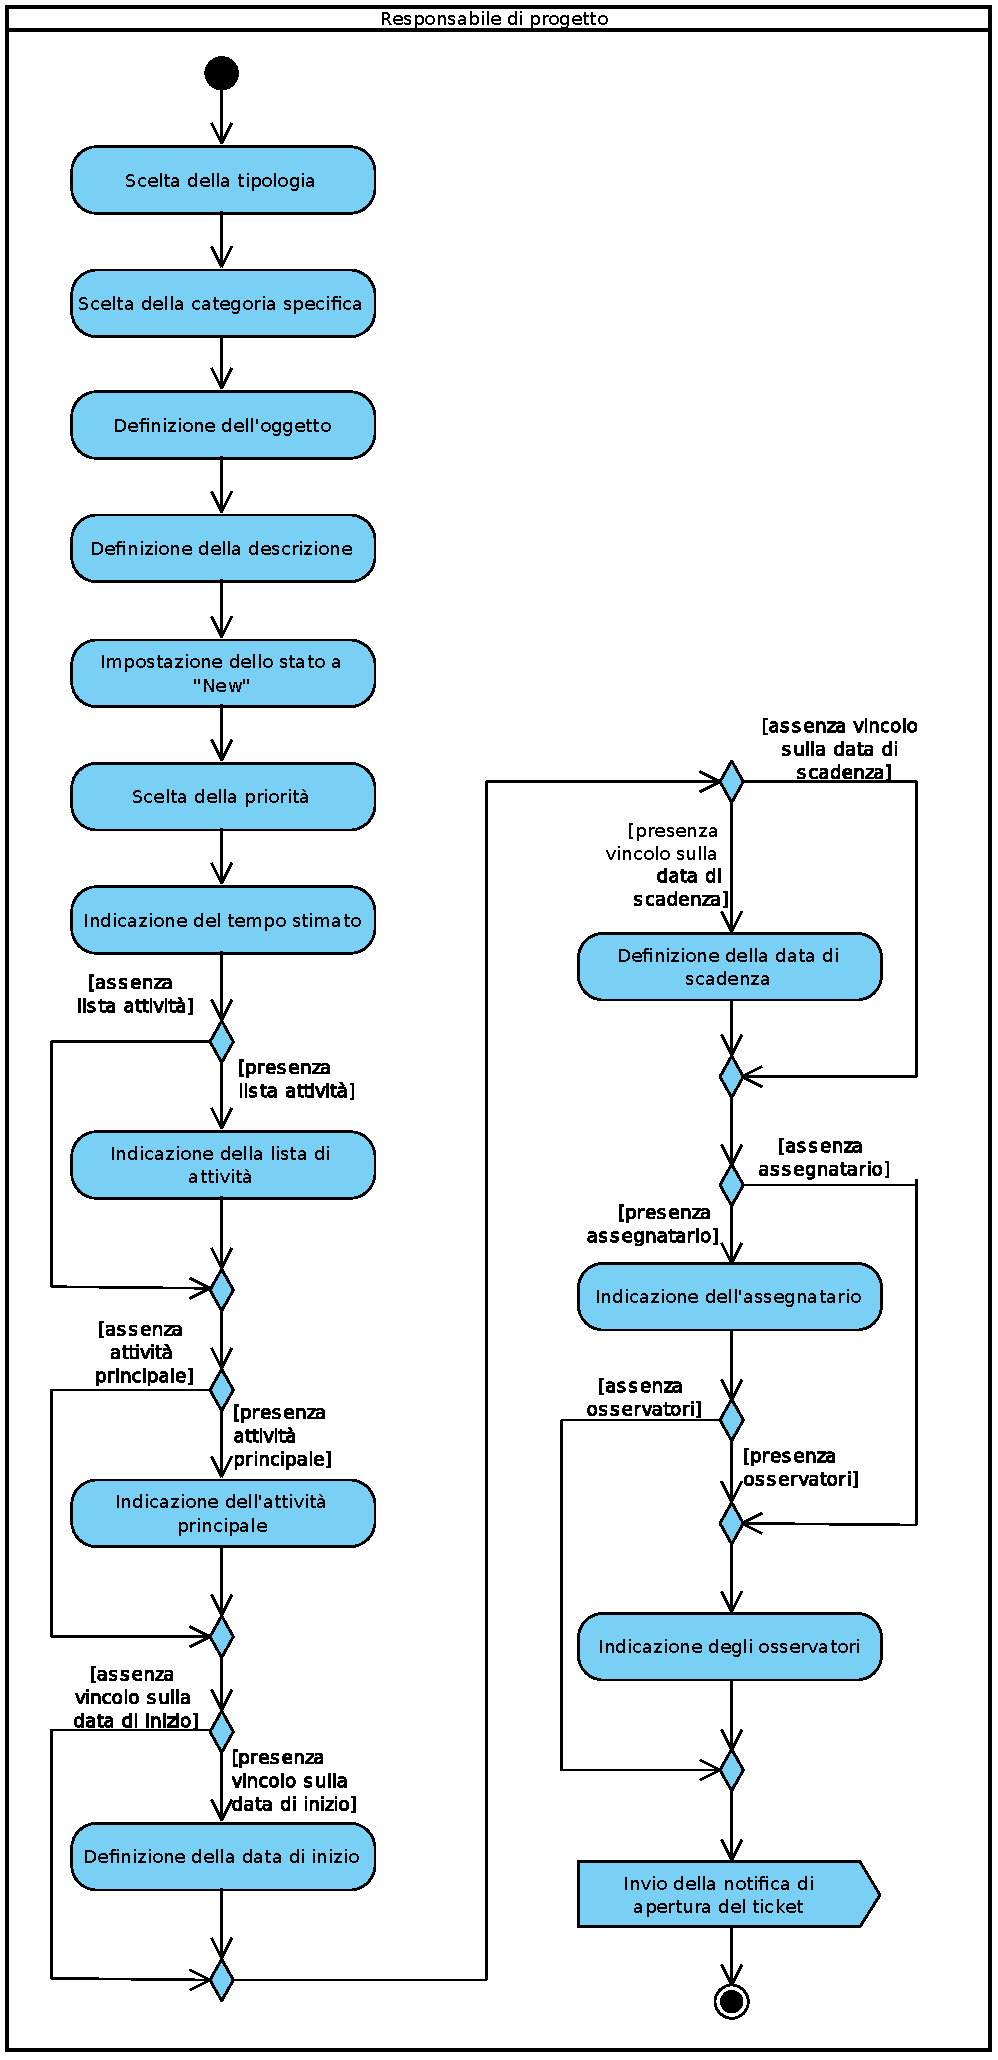
\includegraphics[width=10cm]{../immagini/aperturaTicket.pdf}
\caption{Diagramma di attività - apertura di un ticket}
\label{fig:aperturaTicket}
\end{figure}
\subsubsubsection{Rigetto di un ticket}
La procedura di rigetto di un ticket da parte del \rRP segue il diagramma di attività riportato in \customRef{fig:rigetto_chiusuraTicket}{figura}.
Il \rRP:
\begin{enumerate}
\item Riceve la notifica di un ticket con stato ``Approved'';
\item Effettua una rapida ricerca per trovare eventuali anomalie non catturate dal \rV, che dà esito positivo;
\item Crea una lista con le anomalie trovate;
\item Imposta lo stato del ticket a ``Rejected'' e lo commenta con il link alla lista delle anomalie;
\item Apre i ticket per la correzione delle anomalie;
\item Apre un ticket per la verifica della correzione delle anomalie.
\end{enumerate}
\subsubsubsection{Chiusura di ticket}
La procedura di chiusura di ticket segue il diagramma di attività riportato in \customRef{fig:rigetto_chiusuraTicket}{figura}.
L'attività di chiusura di ticket è delegata al \rRP, che:
\begin{enumerate}
\item Riceve la notifica di un ticket con stato ``Approved'';
\item Effettua una rapida ricerca per trovare eventuali anomalie non catturate dal \rV, che dà esito negativo.
\end{enumerate}
oppure:
\begin{enumerate}
\item Riceve la notifica di un ticket con stato ``Rejected'', accompagnata dalla lista delle anomalie trovate dal verificatore;
\item Apre i ticket per la correzione delle anomalie;
\item Apre un ticket per la verifica della correzione delle anomalie.
\end{enumerate}
Infine, il \rRP imposta lo stato del ticket a ``Closed''.
\begin{figure}[H]
\centering
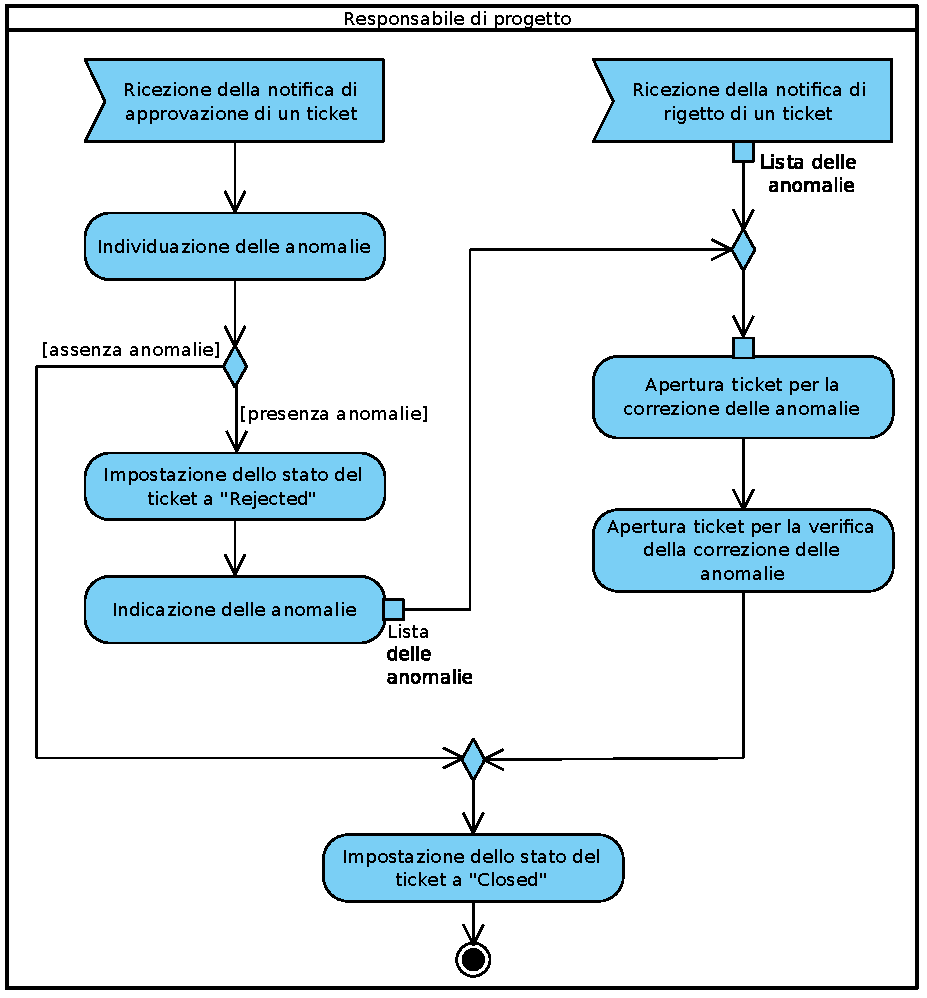
\includegraphics[width=9cm]{../immagini/rigetto_chiusuraTicket.pdf}
\caption{Diagramma di attività - rigetto/chiusura di ticket}
\label{fig:rigetto_chiusuraTicket}
\end{figure}
\subsubsubsection{Rilevazione dei rischi}\label{procRilevazRischi}
In ciascuna fase del \gloxy{progetto}, il \rRP avrà il compito di individuare i rischi indicati nel \PP.
Nel caso si verifichino problematiche non previste, il \rRP dovrà includerle nell’analisi dei rischi.
Complessivamente la procedura di rilevazione dei rischi prevede i seguenti passi:
\begin{enumerate}
\item Rilevazione dei problemi non calcolati;
\item Analisi e classificazione dei nuovi rischi individuati;
\item Pianificazione di controllo dei nuovi rischi individuati;
\item Definizione di contromisure per i nuovi rischi individuati.
\end{enumerate}
\begin{figure}[H]
\centering
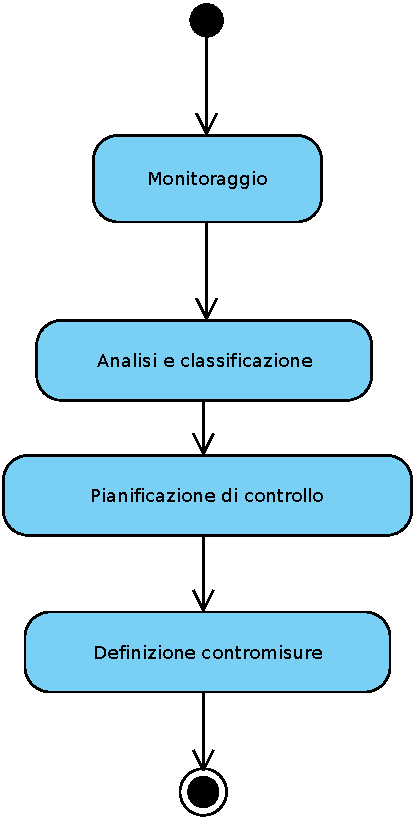
\includegraphics[width=5cm]{../immagini/analisiRischi.pdf}
\caption{Diagramma di attività - rilevazione dei rischi}
\label{fig:rilevazione rischi}
\end{figure}

\subsubsection{Norme}
\subsubsubsection{Template}
Per agevolare e uniformare la redazione dei documenti è stato creato un \gloxy{template} \LaTeX~ contenente tutte le impostazioni stilistiche e i comandi citati in questo documento.\\
Il \gloxy{template} è disponibile nel \gloxy{repository} \texttt{\pragmaDocs} all'interno della cartella \texttt{\nogloxy{template}}.
\subsubsubsection{Norme tipografiche}\label{normeTipografiche}
Questa sezione racchiude le convenzioni adottate da \gruppo per scrivere i documenti in modo uniforme.
\subsubsubsubsection{Norme riguardo nomi}\label{norNome}
Ogniqualvolta si debbano elencare i nomi completi dei componenti del gruppo, tale elenco dovrà essere ordinato lessicograficamente per cognome, e deve sempre essere indicato prima il nome e poi il cognome.
\subsubsubsubsection{Stile del testo}
\begin{itemize}
\item \textbf{Corsivo:} deve essere usato quando ci si riferisce al nome di un documento o a un ruolo, quando si scrivono delle citazioni o abbreviazioni e in tutti gli altri casi in cui si ritiene sia utile mettere in rilievo del testo;
\item \textbf{Grassetto:} può essere usato per evidenziare delle parole chiave oppure per evidenziare il concetto sviluppato da una voce in un elenco puntato;
\item \textbf{\gloxy{Monospace}:} deve essere utilizzato quando si riportano parti di codice, comandi o \gloxy{percorsi} di file;
\item \textbf{Maiuscolo:} l'utilizzo del maiuscolo è riservato solamente per le macro;
\item \textbf{\LaTeX:} per riferirsi a \LaTeX~ è obbligatorio usare l'apposito comando $\backslash$LaTeX.
\end{itemize}
\subsubsubsubsection{Punteggiatura}
\begin{itemize}
\item \textbf{Punteggiatura:} un carattere di punteggiatura non deve mai essere preceduto da un carattere di spaziatura;
\item \textbf{Parentesi:} il testo racchiuso tra parentesi non deve mai iniziare o terminare con un carattere di spaziatura o di punteggiatura, inoltre all'interno del testo racchiuso tra parentesi non deve esserci un altro gruppo di parentesi;
\item \textbf{Lettere maiuscole:} le lettere maiuscole vanno usate per indicare il nome del \gloxy{team}, del \gloxy{progetto}, dei documenti, dei ruoli, delle fasi di lavoro, nelle parole \gloxy{Proponente} e \gloxy{Committente}, all'inizio di un punto di un elenco puntato e in tutte le occasioni in cui ne è previsto l'uso dalla lingua italiana;
\item \textbf{Ritorno a capo:} la decisione riguardo l'uso del ritorno a capo è lasciata a chi scrive il documento, questo perché l'andare a capo dipende dal contesto.
\end{itemize}
Queste convenzioni possono essere trascurate solamente quando si inserisce del codice sorgente all'interno del documento.
\subsubsubsubsection{Composizione del testo}
\begin{itemize}
\item \textbf{Elenchi puntati:} ogni punto dell'elenco deve terminare con un punto e virgola, fatta eccezione per l'ultimo elemento che deve terminare con un punto. La prima parola deve iniziare con una lettera maiuscola, salvo casi particolari in cui è richiesto l'uso della lettera minuscola (es: nome di un file);
\item \textbf{Note a pié pagina:} ogni nota deve cominciare con l'iniziale della prima parola maiuscola e non deve essere preceduta da alcun carattere di spaziatura. Ogni nota deve inoltre terminare con un punto;
\item \textbf{Sigle:} l'uso delle sigle è consentito solamente nei casi in cui sia necessario risparmiare spazio come per esempio nelle tabelle o diagrammi. Le sigle che si prevedono di utilizzare sono:
\begin{itemize}
\item \textbf{AdR:} \AR;
\item \textbf{GL:} \G;
\item \textbf{NdP:} \NP;
\item \textbf{PdP:} \PP;
\item \textbf{PdQ:} \PQ;
\item \textbf{SdF:} \SF;
\item \textbf{ST:} \ST;
\item \textbf{RR:} \RR;
\item \textbf{RP:} \RP;
\item \textbf{RQ:} \RQ;
\item \textbf{RA:} \RA;
\item \textbf{Re:} \rRP;
\item \textbf{Am:} \rAP;
\item \textbf{An:} \rA;
\item \textbf{Pt:} \rP;
\item \textbf{Ve:} \rV;
\item \textbf{Pr:} \rp.
\end{itemize}
\end{itemize}
\subsubsubsubsection{Formati ricorrenti}
\begin{itemize}
\item \textbf{\gloxy{Percorsi}:} per gli indirizzi email e \gloxy{web} deve essere utilizzato il comando $\backslash$url, mentre per gli indirizzi relativi va usato il comando \LaTeX~$\backslash$texttt che usa il formato \gloxy{monospace};
\item \textbf{Date:} le date dovranno seguire il formato
\begin{center}
AAAA-MM-GG
\end{center}
dove:
\begin{itemize}
\item[-] AAAA: rappresenta l'anno scritto utilizzando 4 cifre;
\item[-] MM: rappresenta il mese scritto utilizzando sempre 2 cifre;
\item[-] GG: rappresenta il giorni scritto utilizzando sempre 2 cifre.
\end{itemize}
\item \textbf{Numeri:} i numeri saranno formattati secondo lo standard [SI/ISO 31-0];
\item \textbf{Nome dei file:} per riferirsi ad un file usandone solo il nome è necessario utilizzare il formato \gloxy{monospace};
\item \textbf{Nome dei documenti:} per garantire la scrittura uniforme del nome dei documenti sono stati inseriti dei comandi distinti dalle iniziali maiuscole del nome del documento, ad esempio $\backslash$NP che stampa \NP. \\
Nel caso sia necessario fare riferimento alla versione più aggiornata del documento sono stati predisposti dei comandi \LaTeX~$\backslash$nomeDelDocumento che stampano in modo corretto il nome del documento e l'ultima versione approvata, ad esempio \normeDiProgetto;
\item \textbf{Ruoli di \gloxy{progetto}:} per garantire la scrittura uniforme dei ruoli di \gloxy{progetto} sono stati inseriti dei comandi distinti dalle iniziali maiuscole del nome del ruolo e che hanno come prefisso una ``r'', ad esempio $\backslash$rRP stampo \rRP;
\item \textbf{Revisioni:} per garantire la scrittura uniforme delle revisioni sono stati inseriti dei comandi caratterizzati dalle iniziali maiuscole dei nomi delle revisioni, ad esempio $\backslash$RR stampa \RR;
\item \textbf{Fasi del \gloxy{progetto}:} per garantire la scrittura uniforme del nome delle fasi sono stati inseriti dei comandi caratterizzati dalle iniziali maiuscole del nome delle fasi preceduti da un ``f'', ad esempio $\backslash$fAD stampa \fAD;
\item \textbf{Nomi dei componenti:} per riferirsi ai componenti del \gloxy{team} sono state definite le seguenti macro:
\begin{itemize}
\item[-] \textbf{$\backslash$ao}: \ao;
\item[-] \textbf{$\backslash$fv}: \fv;
\item[-] \textbf{$\backslash$sm}: \sm;
\item[-] \textbf{$\backslash$mb}: \mb;
\item[-] \textbf{$\backslash$dm}: \dm;
\item[-] \textbf{$\backslash$gmi}: \gmi;
\item[-] \textbf{$\backslash$gma}: \gma.
\end{itemize}
\item \textbf{Nome del gruppo:} ci si riferirà al gruppo solamente con il nome \gruppo , per scrivere in modo corretto il nome è stata definita la macro $\backslash$gruppo;
\item \textbf{Nome del \gloxy{Proponente}:} ci si riferirà al \gloxy{Proponente} come ``\proponente'' o con ``Proponente''. Per la corretta scrittura è stata definita la macro $\backslash$proponente;
\item \textbf{Nome del referente del \gloxy{Proponente}:} ci si riferirà al referente del \gloxy{Proponente} come ``\referenteProponente'' o con ``Referente \proponente''. Per la corretta scrittura è stata definita la macro $\backslash$referenteProponente;
\item \textbf{Nome del \gloxy{Committente}:} ci si riferirà al \gloxy{Committente} come ``\committente'' o con ``Committente''. Per la corretta scrittura è stata definita la macro $\backslash$committente;
\item \textbf{Nome del \gloxy{progetto}:} ci si riferirà al \gloxy{progetto} solo come ``\progetto'' . Per la corretta scrittura è stata definita la macro $\backslash$progetto.
\end{itemize}
Un file con i comandi appena descritti è reperibile al seguente link: \\
\url{https://docs.google.com/document/d/1dRy2r-Ewp7Ye8iP-YKJz3T5XkkRIbCOZEPJ-aZocWK4/edit}
\subsubsubsection{Componenti grafiche}
\subsubsubsubsection{Tabelle}
Ad ogni tabella presente all'interno dei documenti deve essere associata una didascalia e un numero identificativo incrementale al fine di renderla tracciabile all'interno del documento.
\subsubsubsubsection{Immagini}
Il formato preferibile per le immagini è \gloxy{PDF}, ma qualora non fosse disponibile è desiderabile l'uso de formato \gloxy{PNG}.
\subsubsubsection{Struttura dei documenti}
\subsubsubsubsection{Frontespizio}
La prima pagina di ogni documento contiene, nell'ordine, le seguenti informazioni:
\begin{itemize}
\item Nome del \gloxy{progetto};
\item Logo e nome del gruppo;
\item Titolo del documento;
\item Versione del documento
\item Nome e cognome dei redattori del documento;
\item Nome e cognome dei \rVs del documento;
\item Nome e cognome del \rRP, che dovrà approvare il documento;
\item Uso del documento;
\item Lista di distribuzione del documento;
\item Descrizione del documento;
\item Anno accademico;
\item Mail del \gloxy{team}.
\end{itemize}
\subsubsubsubsection{Diario delle modifiche}\label{diarioModifiche}
La seconda pagina di ogni documento contiene il diario delle modifiche, cioè una tabella contenente le seguenti informazioni:
\begin{itemize}
\item Data della modifica;
\item Descrizione delle modifiche effettuate; specificandone, quando possibile, le sezioni interessate, e segnalando eventuali riferimenti a sezioni di documenti esterni coinvolti (per riferirsi a decisioni prese in verbali ufficiali si veda la \customRef{verbaliUfficiali}{sezione});
\item Nome e cognome dell'autore;
\item Ruolo ricoperto all'interno del gruppo dall'autore della modifica;
\item Versione del documento dopo la modifica.
\end{itemize}
Le righe della tabella saranno ordinate per data decrescente, in modo che la prima riga della tabella corrisponda all'ultima modifica effettuata.
\subsubsubsubsection{Indici}
Dopo il diario delle modifiche è presente l'indice delle sezioni, e a seguire, solo nel caso siano presenti figure o tabelle, gli indici delle figure e delle tabelle.
\subsubsubsubsection{Struttura generale di una pagina}
L'intestazione di ogni pagina contiene:
\begin{itemize}
\item Il nome del gruppo;
\item La sezione corrente del documento.
\end{itemize}
Il pié di pagina contiene:
\begin{itemize}
\item Il nome del documento;
\item Il numero di pagina corrente espresso nella forma \textit{Pagina: X / Y}, dove X è il numero di pagina corrente e Y è il numero di pagine totali.
\end{itemize}
\subsubsubsection{Tipi di documenti}
\subsubsubsubsection{Documenti interni}
Rappresentano documenti redatti per un utilizzo interno a \gruppo, che non devono essere distribuiti all'esterno e
che non necessitano di \gloxy{versionamento}. Questa tipologia di documentazione verrà archiviata su \gloxy{Google Drive}.
A questa categoria di documenti appartengono le bozze di documento e i verbali interni informali.
\subsubsubsubsubsection{Verbali interni informali}
Un verbale interno informale è un documento che descrive gli argomenti discussi durante una riunione tra soli membri del \gloxy{team}, che dovrà restare a loro esclusiva disposizione. Verrà redatto da un membro del \gloxy{team}, condiviso mediante \gloxy{Google Drive}, e inviato a tutti i suoi componenti tramite posta elettronica.
\subsubsubsubsubsection{Bozze di documenti ufficiali}
Per velocizzare la stesura dei documenti informali è possibile iniziare a scrivere un bozza,
in  modo che anche i membri del gruppo che non sono familiari con \LaTeX~ possano iniziare a produrre materiale fin da subito.
Quando viene creata una bozza è necessario comunicarlo in \gloxy{mailing list} usando come oggetto:
\begin{center}
\texttt{[Bozza] Nome del documento}
\end{center}
In ogni caso è necessario che la bozza sia promossa a documento informale il prima possibile.
\subsubsubsubsection{Documenti ufficiali}
\subsubsubsubsubsection{Verbali ufficiali}\label{verbaliUfficiali}
Un verbale ufficiale è un documento che descrive gli argomenti discussi durante una riunione con il \gloxy{Proponente} (verbale interno) o con il \gloxy{Committente} (verbale esterno), ed ha quindi valore normativo.
\\Ogni sezione del documento dovrà essere dedicata ad un particolare problema trattato all'incontro, che dovrà essere presentato e ne dovrà essere descritta la relativa decisione presa con il \gloxy{Committente}.
\\Il documento dovrà essere consultabile dal \gloxy{team} e dalle parti esterne, quindi verrà allegato ad un messaggio di risposta alla mail di convocazione della riunione esterna e inviato alla \gloxy{mailing list} del \gloxy{team}.
Per agevolarne l'identificazione, i verbali interni verranno denominati con un codice univoco \emph{TN}, dove:
\begin{itemize}
\item \emph{T} rappresenta il tipo del verbale: \emph{E}, per i verbali esterni relativi a riunioni tenute con il \gloxy{Committente}, e \emph{I}, per i verbali interni relativi a riunioni con il \gloxy{Proponente};
\item \emph{N} è un numero intero che parte da \emph{1} e viene incrementato per ogni nuovo verbale di tipo \emph{T} di verbale.
\end{itemize}
Per riferirsi ad una precisa decisione di un verbale ufficiale\footnote{I verbali dovranno comparire anche tra i riferimenti normativi del documento.}, è sufficiente indicare il codice univoco del verbale seguito da un trattino e dal numero della decisione interessata. Per fare ciò si deve utilizzare la notazione \emph{TN-D}, dove \emph{TN} è il codice dell’\emph{N}-esimo verbale ufficiale e \emph{D} è la \emph{D}-esima decisione.
\subsubsubsubsubsection{Documenti informali}
Un documento è ritenuto informale finché non viene approvato dal \rRP.
Appartengono a questa categoria tutti i documenti che dovranno essere consegnati al \gloxy{Committente} o al \gloxy{Proponente},
questi documenti sono memorizzati nel \gloxy{repository} \texttt{\pragmaDocs} e devono attenersi alle \NP.
\subsubsubsubsubsection{Documenti formali}
Un documento diventa formale quando viene approvato dal \rRP.
Per raggiungere questo stato è necessario che il documento sia conforme alle \NP e che abbia seguito il \gloxy{percorso} di verifica e validazione in esse descritto.
\subsubsubsubsubsection{\G}
Il \G conterrà le \emph{parole} dei documenti che possono far parte del contesto dell'applicazione e i \emph{termini} che possono generare ambiguità d'interpretazione. Tali termini saranno disposti in ordine alfabetico ed ognuno di essi avrà una definizione, che dovrà essere sintetica e precisa, per non creare equivoci o ambiguità.
Ogni membro del \gloxy{team} è invitato a inserire nel \G le parole da esso individuate, delle quali non esista ancora una definizione. L'inserimento dei termini nel \G avverrà parallelamente alla stesura dei documenti sfruttando le funzionalità offerte da \pragmadb.
%I termini verranno inseriti nel \G parallelamente alla stesura degli altri documenti, in modo da evitare errori umani.\\
\subsubsubsection{Versionamento}\label{versionamento}
L'avanzamento di versione da parte dei documenti sarà espresso nella seguente forma:
\begin{center}
vX.Y.Z
\end{center}
dove:
\begin{itemize}
\item \textbf{X}: indica il numero di uscite formali del documento e viene incrementato in corrispondenza con l'ultima approvazione del \rRP prima del rilascio. L'incremento di \textbf{X} comporta l'azzeramento sia di \textbf{Y} che di \textbf{Z};
\item \textbf{Y}: indica il numero di modifiche e correzioni effettuate al documento. L'incremento \textbf{Y} comporta l'azzeramento di \textbf{Z};
\item \textbf{\textbf{Z}}: quando vale\begin{itemize}[label=\ding{212}]
\item 0: indica che le ultime modifiche (successive all'ultima verifica) non sono state verificate;
\item 1: indica che le ultime modifiche (successive all'ultima verifica) sono state verificate;
\item 2: indica che l'ultima verifica è stata approvata.
\end{itemize}
\end{itemize}
Quando si fa riferimento al contenuto di una specifica versione di un documento, ne è richiesta la sua precisazione usando la seguente sintassi:
\begin{center}
\textit{NomeDocumento vX.Y.Z}
\end{center}
Quando saranno creati i file, il loro nome dovrà seguire lo schema:
\begin{center}
\texttt{nomeDocumento\_vX.Y.Z.pdf}
\end{center}

\subsubsection{Strumenti}
\subsubsubsection{\pragmadb}\label{PragmaDB}
\pragmadb è un'applicazione \gloxy{web} sviluppata dal \gloxy{team} per la gestione di casi d'uso, attori, fonti, requisiti e termini del \G. Il suo scopo è velocizzare e automatizzare la gestione dei dati, e semplificare i tracciamenti. Ogni membro del \gloxy{team} può accedere all'applicazione via \gloxy{browser} previa autenticazione, inoltre, più persone possono lavorare simultaneamente sugli stessi dati poiché è stata gestita la concorrenza. L'applicazione si occupa di mantenere ordinata la gerarchia dei requisiti e degli UC in modo automatico durante tutto il suo ciclo di vita (creazione, modifica, eliminazione).\\
Vengono eseguiti diversi controlli su ciascun campo dati, e tale approccio garantisce \gloxy{fault-tolerance} del sistema nei confronti di qualsiasi input possibile. I membri del gruppo possono visualizzare, inserire, modificare ed eliminare elementi in modo semplice. \pragmadb consente di esportare l'elenco degli attori, delle fonti, del \G, dei casi d'uso, dei requisiti e delle loro relazioni come codice \LaTeX, quindi facilmente inseribile all'interno dei documenti durante la stesura. Infine consente di visualizzare, attraverso un menù laterale, l'insieme dei link utili relativi al gruppo (link al \gloxy{repository}, link al foglio dei comandi \LaTeX, link a Redmine, link alla \gloxy{mailing list} Yahoo).
\subsubsubsubsection{Attori}
La sezione degli attori è pensata per mantenere traccia di tutti gli attori del sistema.
Un attore è caratterizzato da un nome identificativo e da una descrizione. \`{E} possibile inserire, modificare o eliminare attori, ed esportare in \LaTeX\ una tabella contenente tutte le informazioni su di essi.
Cliccando sul nome di un attore è possibile vederne il dettaglio dello stesso, che mostra in particolare, una lista dei casi d'uso correlati, per facilitarne il processo di verifica.
\`E consentita l'eliminazione di un attore solamente se non esiste alcun caso d'uso ad essa riferito.
\subsubsubsubsection{Fonti}
La sezione delle fonti è pensata per mantenere traccia di tutte le fonti (capitolati, verbali, ecc\dots) che hanno determinato l'individuazione di un requisito.
Una fonte è caratterizzata da un identificativo, un nome e una descrizione. \`{E} possibile inserire, modificare o eliminare fonti, ed esportare in \LaTeX\ una tabella contenente tutte le informazioni su di esse.
Cliccando sull'identificativo di una fonte è possibile vederne il dettaglio dello stesso, che mostra in particolare, una lista dei requisiti correlati, per facilitarne il processo di verifica.
\`E consentita l'eliminazione di una fonte solamente se non esiste alcun requisito derivato da essa.
\subsubsubsubsection{Requisiti}
La sezione dei requisiti è pensata per mantenere traccia di tutti i requisiti individuati.
Un requisito è caratterizzato da un identificativo, un tipo (funzionale, di vincolo, di qualità, prestazionale), un livello di importanza (obbligatorio, desiderabile, facoltativo),
un requisito padre (se non è radice), uno stato (accettato/non accettato + soddisfatto/non soddisfatto + implementato/non implementato), una o più fonti di riferimento e una descrizione. \`{E} possibile inserire, modificare o eliminare requisiti, ed esportare in \LaTeX\ una tabella contenente tutte le informazioni su di essi.
Cliccando sull'identificativo di un requisito è possibile vederne il dettaglio dello stesso, che mostra in particolare, una lista dei requisiti figli e dei casi d'uso correlati, per facilitarne il processo di verifica.
\`E inoltre presente una funzionalità che permette di vedere quali requisiti non sono correlati ad alcun caso d'uso.
\subsubsubsubsection{Casi d'uso}
La sezione dei casi d'uso è pensata per mantenere traccia di tutti i casi d'uso individuati dagli \rAs.
Un caso d'uso è caratterizzato da un identificativo, un nome, un diagramma, una o più precondizioni, una o più postcondizioni, un caso d'uso padre (se non è radice), uno scenario principale, una o più inclusioni (facoltativo), una o più estensioni (facoltativo), uno o più scenari alternativi (facoltativo) e una descrizione. \`{E} possibile inserire, modificare o eliminare casi d'uso, ed esportare in \LaTeX\ una tabella contenente tutte le informazioni su di essi.
Cliccando sull'identificativo di un caso d'uso è possibile vederne il dettaglio dello stesso, che mostra in particolare, una lista dei casi d'uso figli e dei requisiti correlati, per facilitarne il processo di verifica.
\`E inoltre presente una funzionalità che permette di vedere quali casi d'uso non sono correlati ad alcun requisito.
\subsubsubsubsection{\G}
Nell'area dedicata alla gestione del \G è possibile inserire, modificare o eliminare termini, ed esportare in \LaTeX\ l’intero \G sotto forma di lista di \texttt{newglossaryentry}, macro fornita dal package \texttt{glossaries} di \LaTeX.
Una voce di \G è caratterizzata da un \emph{identificativo}, un \emph{nome} singolare che verrà mostrato nel \G, una descrizione, un \emph{plurale} (facoltativo) per indicare la sua forma plurale, una forma \emph{estesa} (facoltativo) per indicare la forma singolare (più rara) che il termine può assumere alla sua prima occorrenza all'interno dei documenti, una forma \emph{estesa plurale} (facoltativo) per indicare la forma plurale (più rara) che il termine può assumere alla sua prima occorrenza nei documenti e un \emph{sinonimo} (facoltativo).
\subsubsubsubsection{Package e Classi}\label{pdbPackageClassi}
Per ciascun componente (package o classe) è possibile specificare:
\begin{itemize}
\item Un diagramma \gloxy{UML};
\item Una descrizione testuale del componente;
\item Una descrizione del contesto d'utilizzo;
\item Le relazioni con gli altri componenti;
\item I requisiti che il componente va a soddisfare.
\end{itemize}
Per le classi è inoltre possibile specificare gli attributi e i metodi che le caratterizzano e l'eventuale gerarchia di classi a cui appartengono. Alcuni screenshot esemplificativi di queste funzionalità sono stati inseriti nell'\customRef{screenPDB}{appendice}.
\subsubsubsubsection{Test}\label{pdbTest}
In questa sezione è possibile inserire i test definiti dai \rPs{}. Ogni test è caratterizzato da un tipo e una descrizione.
I tipi di test sono: validazione, sistema, integrazione oppure unità; e in base a tale tipo, un test può essere associato a un requisito, a un componente oppure a un metodo di una classe.
%L'associazione tra il test e l'elemento è \emph{1 a 1}: ad un test può essere associato un solo elemento e viceversa.\\
Ogni test è caratterizzato da un id univoco, calcolato automaticamente da \pragmadb e da una serie di parametri che specificano se il test è stato implementato, eseguito e superato.
\subsubsubsubsection{Tracciamento} \label{pragmadbTracciamento}
\pragmadb consente di esportare direttamente in \LaTeX\ molte parti dei documenti
del \gloxy{progetto}, automatizzandone il processo di stesura. Grazie ad uno script
appositamente creato è possibile in ogni momento scaricare tutti i file \LaTeX, inserendoli
nelle cartelle dei rispettivi documenti.
\pragmadb consente il tracciamento delle seguenti coppie di elementi:
\begin{itemize}
\item Requisiti - Fonti;
\item Fonti - Requisiti;
\item Componenti - Requisiti;
\item Requisiti - Componenti;
\item Classi - Requisiti;
\item Requisiti - Classi;
\item Elemento - Test;
\item Test - Elemento.
\end{itemize}
\subsubsubsubsection{Funzionalità di supporto}\label{pdbSupport}
Per semplificare la verifica del tracciamento tra gli elementi memorizzati in \pragmadb, sono state aggiunte funzionalità che permettono di ottenere una lista degli elementi non relazionati con nessun altro elemento. \\
In particolare \pragmadb fornisce la lista di:
\begin{itemize}
\item Requisiti non sono derivati da casi d'uso;
\item Casi d'uso che non generano requisiti;
\item Package che non soddisfano requisiti;
\item Classi che non soddisfano requisiti;
\item Test che non verificano classi o requisiti.
\end{itemize}
\subsubsubsection{WebStorm}
L'ambiente di sviluppo integrato (IDE) utilizzato è \textbf{\gloxy{WebStorm}}. Sono stati testati anche altri \gloxy{IDE}, ma nessuno si è dimostrato all'altezza di \textbf{\gloxy{WebStorm}}. Esso presenta le seguenti funzionalità:
\begin{itemize}
\item Autocompletamento del codice \gloxy{JavaScript}, \gloxy{HTML} 5 e CSS3;
\item Autocompletamento per metodi, funzioni e \gloxy{framework} esterni, utili per il \gloxy{progetto};
\item Debugger \gloxy{JavaScript};
\item Consente di effettuare unit test per \gloxy{JavaScript} mediante il \gloxy{framework} \textbf{\gloxy{Karma}};
\item Compila automaticamente i file \gloxy{Sass} in \gloxy{CSS};
\item Tiene traccia dei cambiamenti effettuati sui file, consentendo di visualizzare lo storico delle modifiche locali e ritornare a versioni precedenti in caso di modifiche o perdite accidentali.
\end{itemize}

\appendix
\begin{appendices}
\section{Lista degli errori frequenti}\label{erroriFrequenti}
\begin{itemize}
\item Norme stilistiche:
\begin{itemize}
\item Mancato rispetto delle norme relative a elenchi puntati e numerati;
\item Mancato utilizzo delle macro;
\item Mancato rispetto delle norme relative alla redazione del diario;
\item Mancata precisazione della versione nei riferimenti a documenti esterni.
\end{itemize}
\item Linguistica:
\begin{itemize}
\item Mancato rispetto degli accenti: uso dell'accento acuto quando è richiesto quello grave, in particolare ``è'' confusa con ``é'';
\item ``HTML'', ``URL'', ``URI'' sono acronimi, vanno con tutte le lettere maiuscole;
\item Periodi eccessivamente lunghi, che complicano la lettura;
\item Errato uso delle doppie, in particolare raddoppio della lettera z davanti a parole che finiscono in ``-ione'';
\item Mancato rispetto della terza persona singolare del congiuntivo presente;
\item Mancato uso dei pronomi, per evitare la ripetizione di una componente della frase;
\item Non si scrive ``Lo scopo è quello di definire \dots'' ma ``Lo scopo è definire \dots'';
\item Uso errato delle persone dei verbi, in particolare persone singolari usate al posto di quelle plurali, a causa di un'errata individuazione del relativo soggetto all'interno delle frasi;
\item Uso errato dei pronomi relativi, in particolare ``il/di/in/a cui'' usati al posto di ``i/dei/nei/ai quali'' e ``le/delle/nelle/alle quali''.
\end{itemize}
\item \LaTeX:
\begin{itemize}
\item Per inserire caratteri speciali, quali ``\$'' e ``\&'', è necessario inserire il prefisso ``\textbackslash'', ad esempio ``\textbackslash\$'' e ``\textbackslash\&'';
\item La maiuscola della lettera ``è'' si scrive ``\textbackslash\ $\grave{}$ E'' oppure ``\textbackslash\ $\grave{}$ \{E\}''.
\end{itemize}
\end{itemize}

\section{Screenshot Redmine}
\begin{figure}[H]
\centering
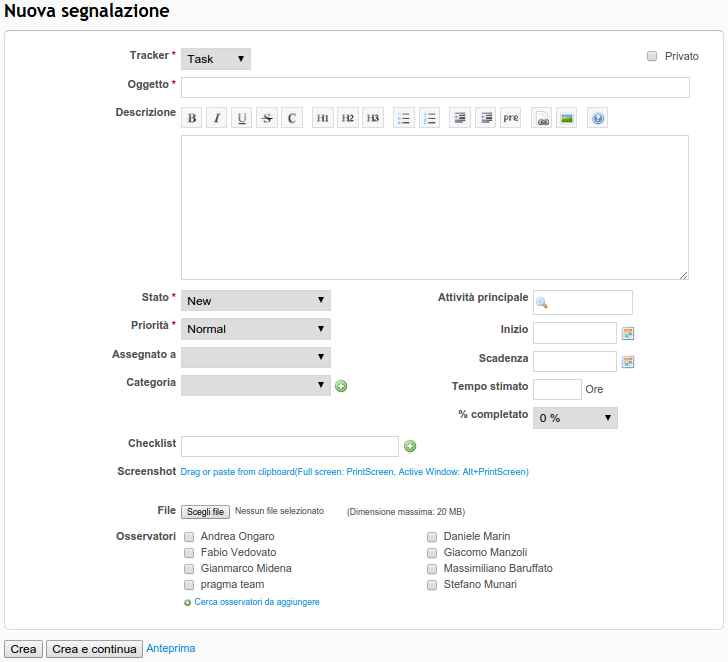
\includegraphics[width=14cm]{../immagini/nuovoTicket.png}
\caption{Form di creazione di un ticket}
\label{fig:assegnazioneTicket}
\end{figure}
%---------
\section{Screenshot \pragmadb}\label{screenPDB}
\begin{figure}[h]
\centering
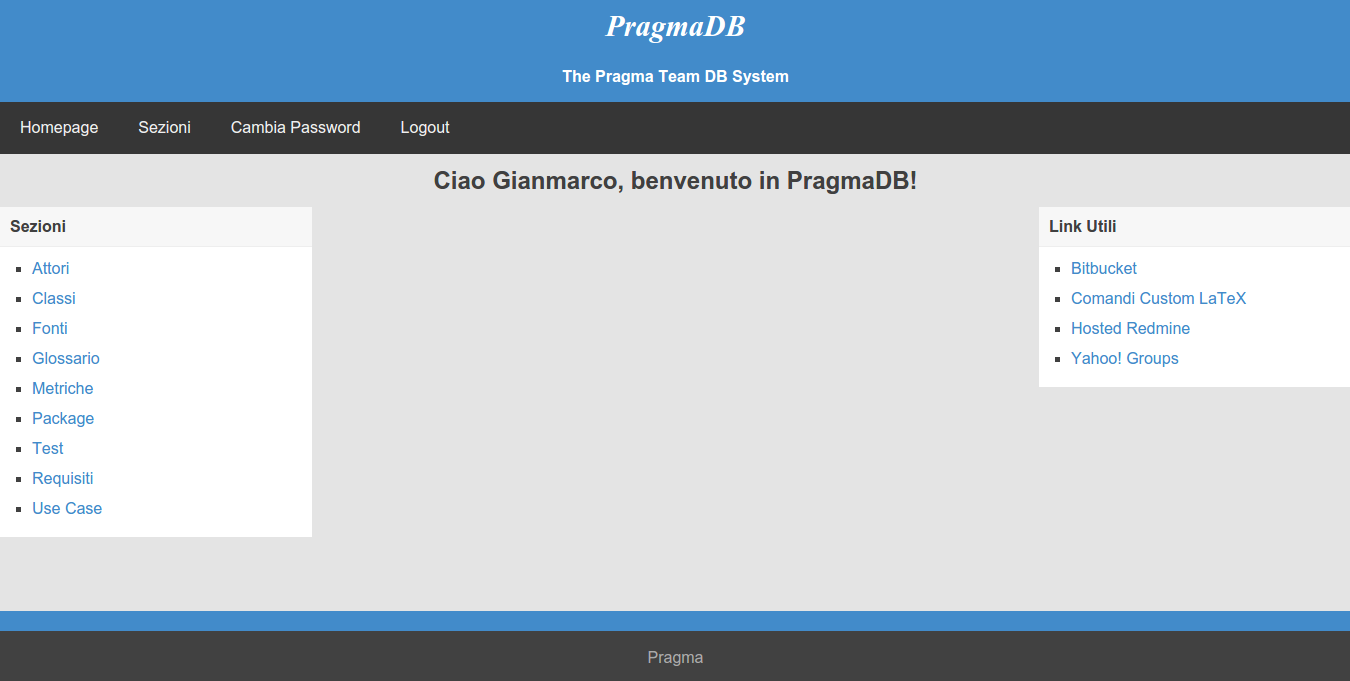
\includegraphics[width=\textwidth,keepaspectratio]{../immagini/home.png}
\caption{\pragmadb\ - pagina principale}\label{fig: PDBHome}
\end{figure}
%---------
\begin{figure}[h]
\centering
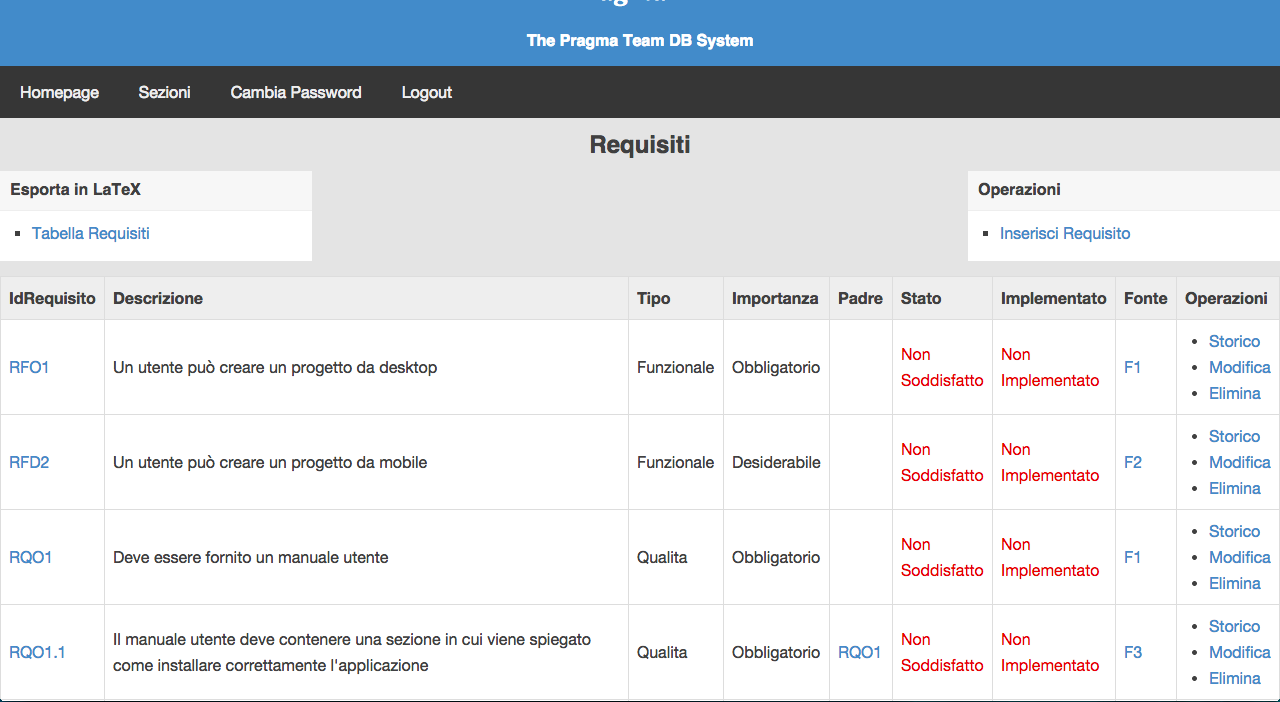
\includegraphics[width=\textwidth,keepaspectratio]{../immagini/requisiti.png}
\caption{\pragmadb\ - pagina dei requisiti}\label{fig: PDBRequisiti}
\end{figure}
%---------
\begin{figure}[h]
\centering
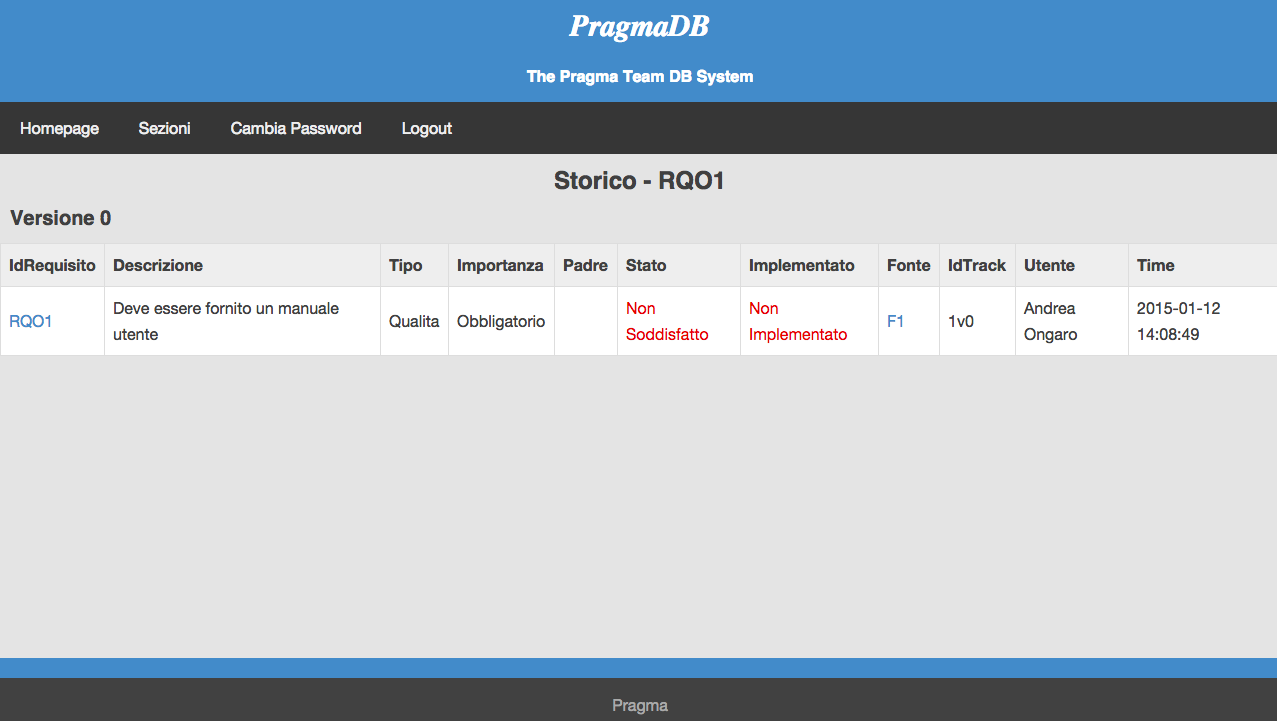
\includegraphics[width=\textwidth,keepaspectratio]{../immagini/history.png}
\caption{\pragmadb\ - pagina dello storico di uno specifico requisito}\label{fig: PDBHistory}
\end{figure}
%---------
\begin{figure}[h]
\centering
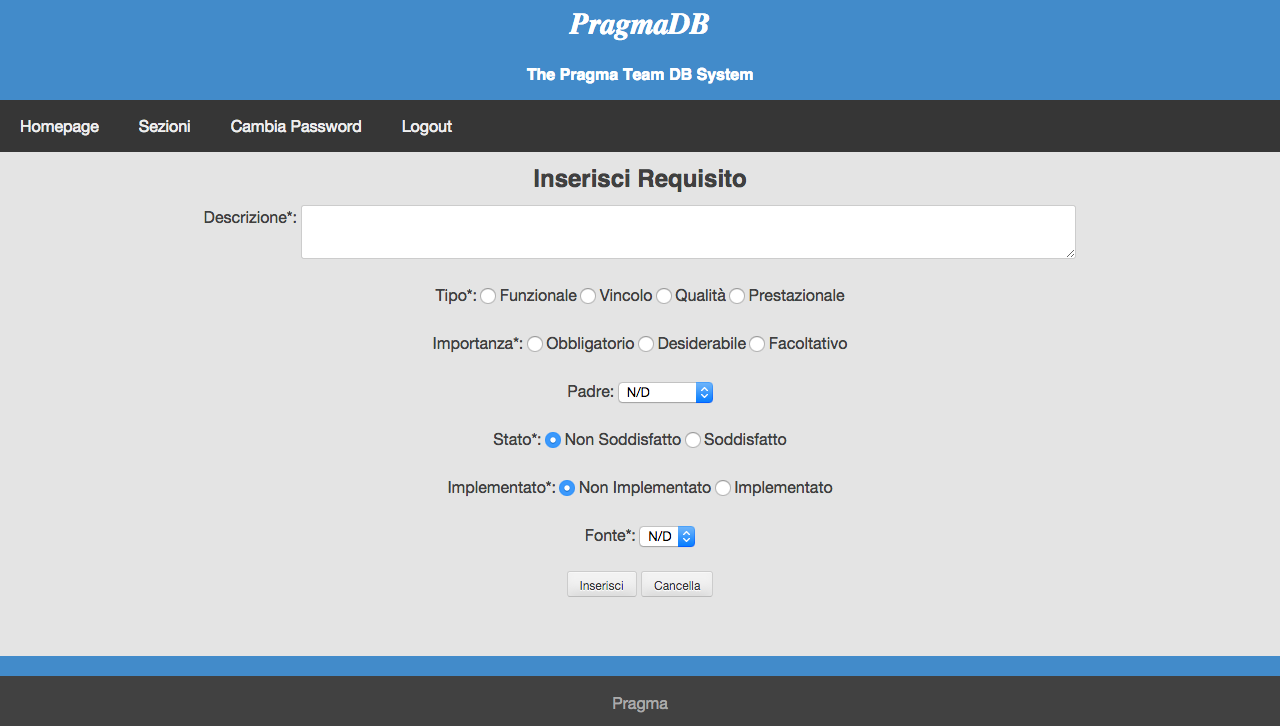
\includegraphics[width=\textwidth,keepaspectratio]{../immagini/insertReq.png}
\caption{\pragmadb\ - pagina di inserimento di un requisito}\label{fig: PDBInsert}
\end{figure}
%---------
\begin{figure}[h]
\centering
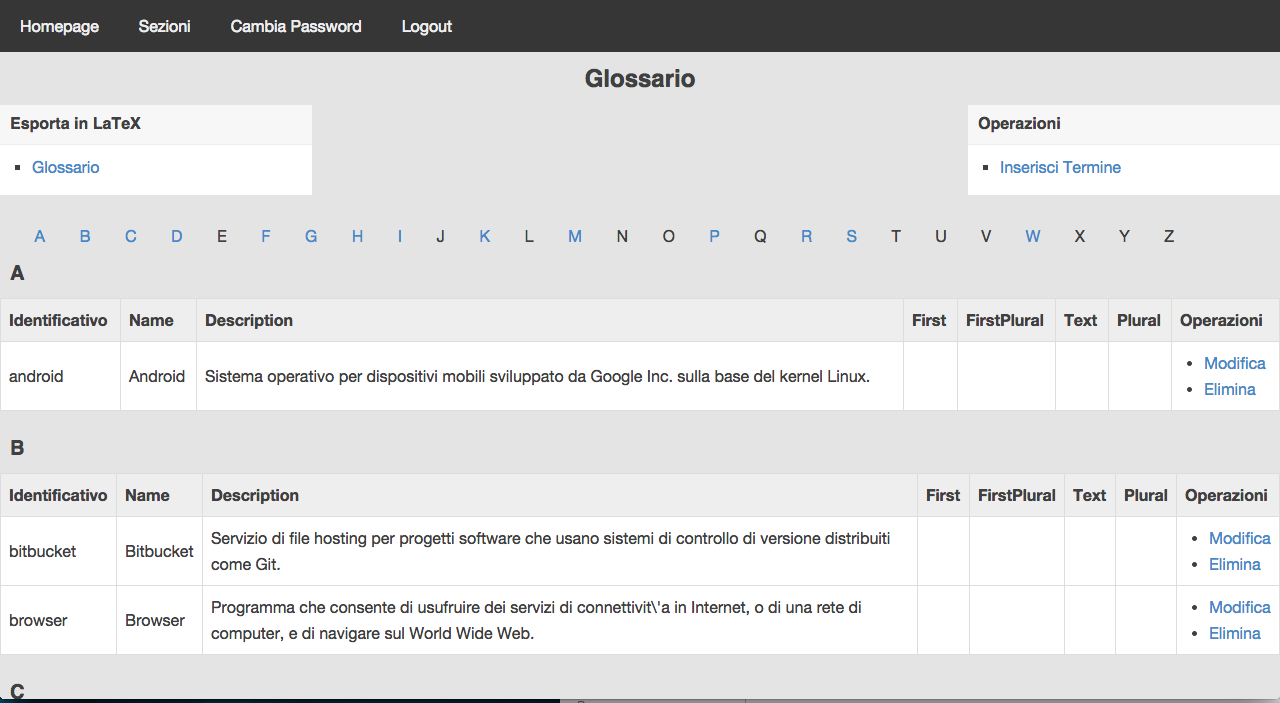
\includegraphics[width=\textwidth,keepaspectratio]{../immagini/glossario.png}
\caption{\pragmadb\ - pagina del \G}\label{fig: PDBGlossario}
\end{figure}
%---------
\begin{figure}[h]
\centering
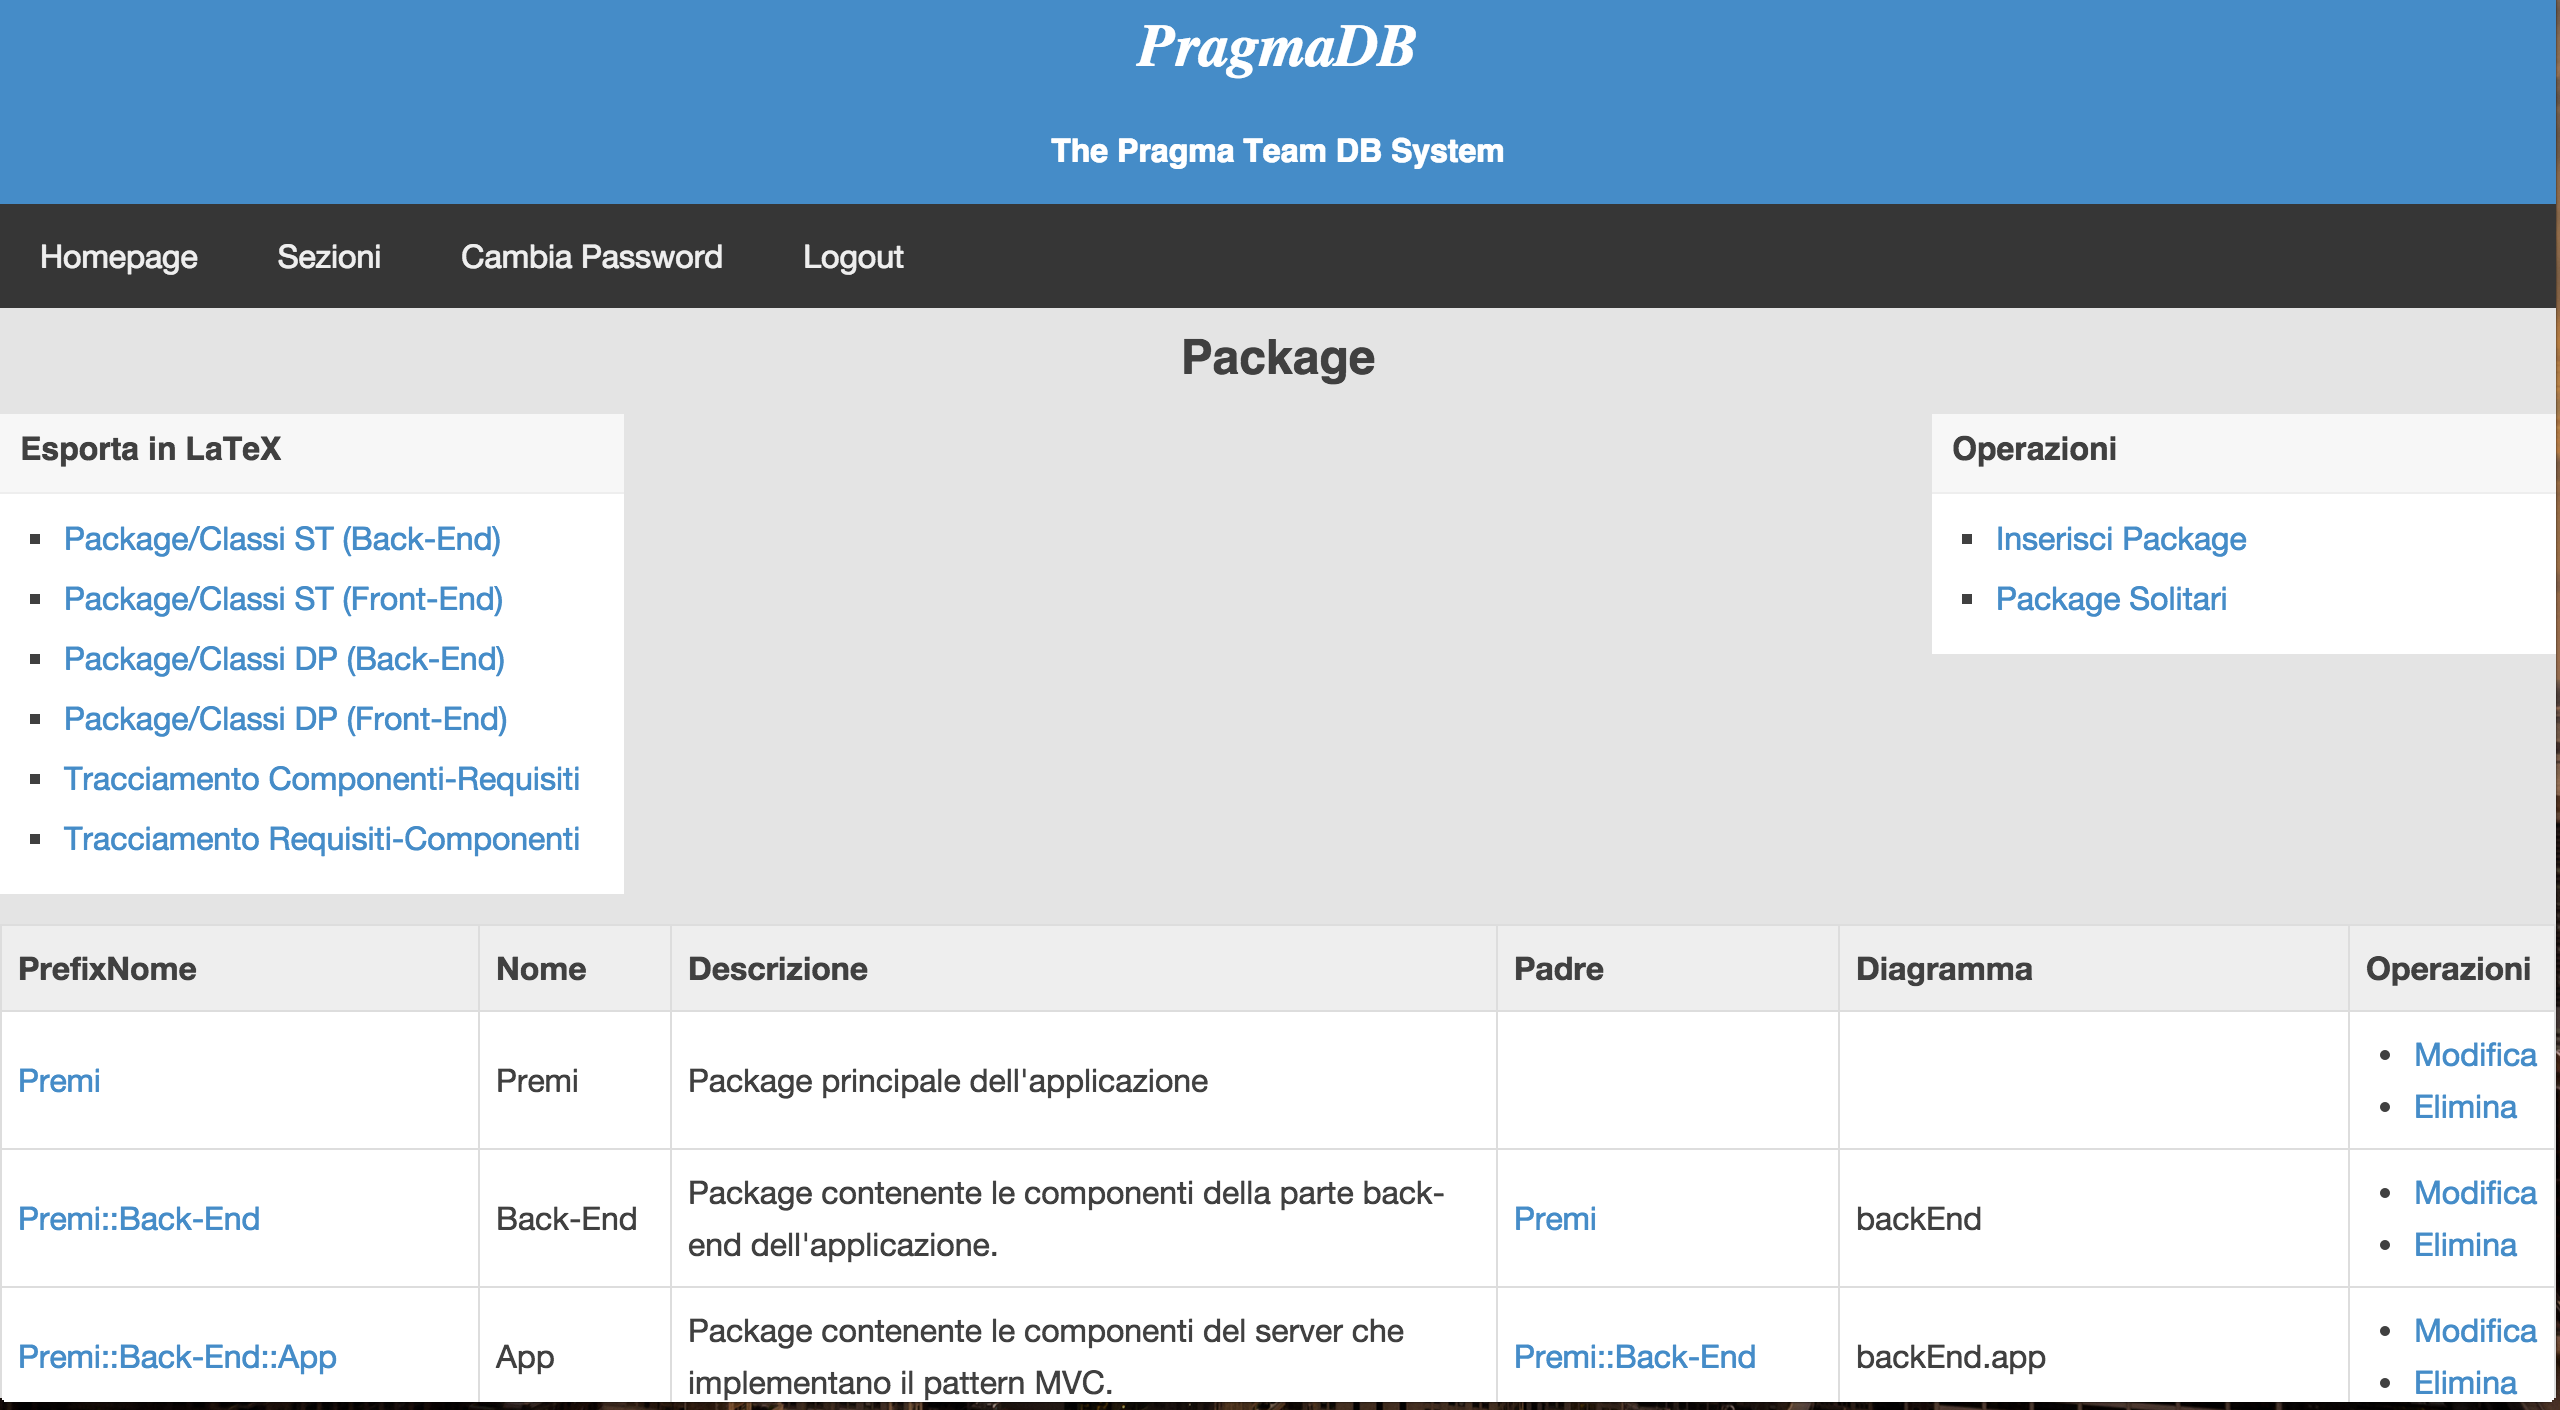
\includegraphics[width=\textwidth,keepaspectratio]{../immagini/pragmadbPackage.png}
\caption{\pragmadb\ - pagina dei package}\label{fig: PDBGlossario}
\end{figure}
%---------
\begin{figure}[h]
\centering
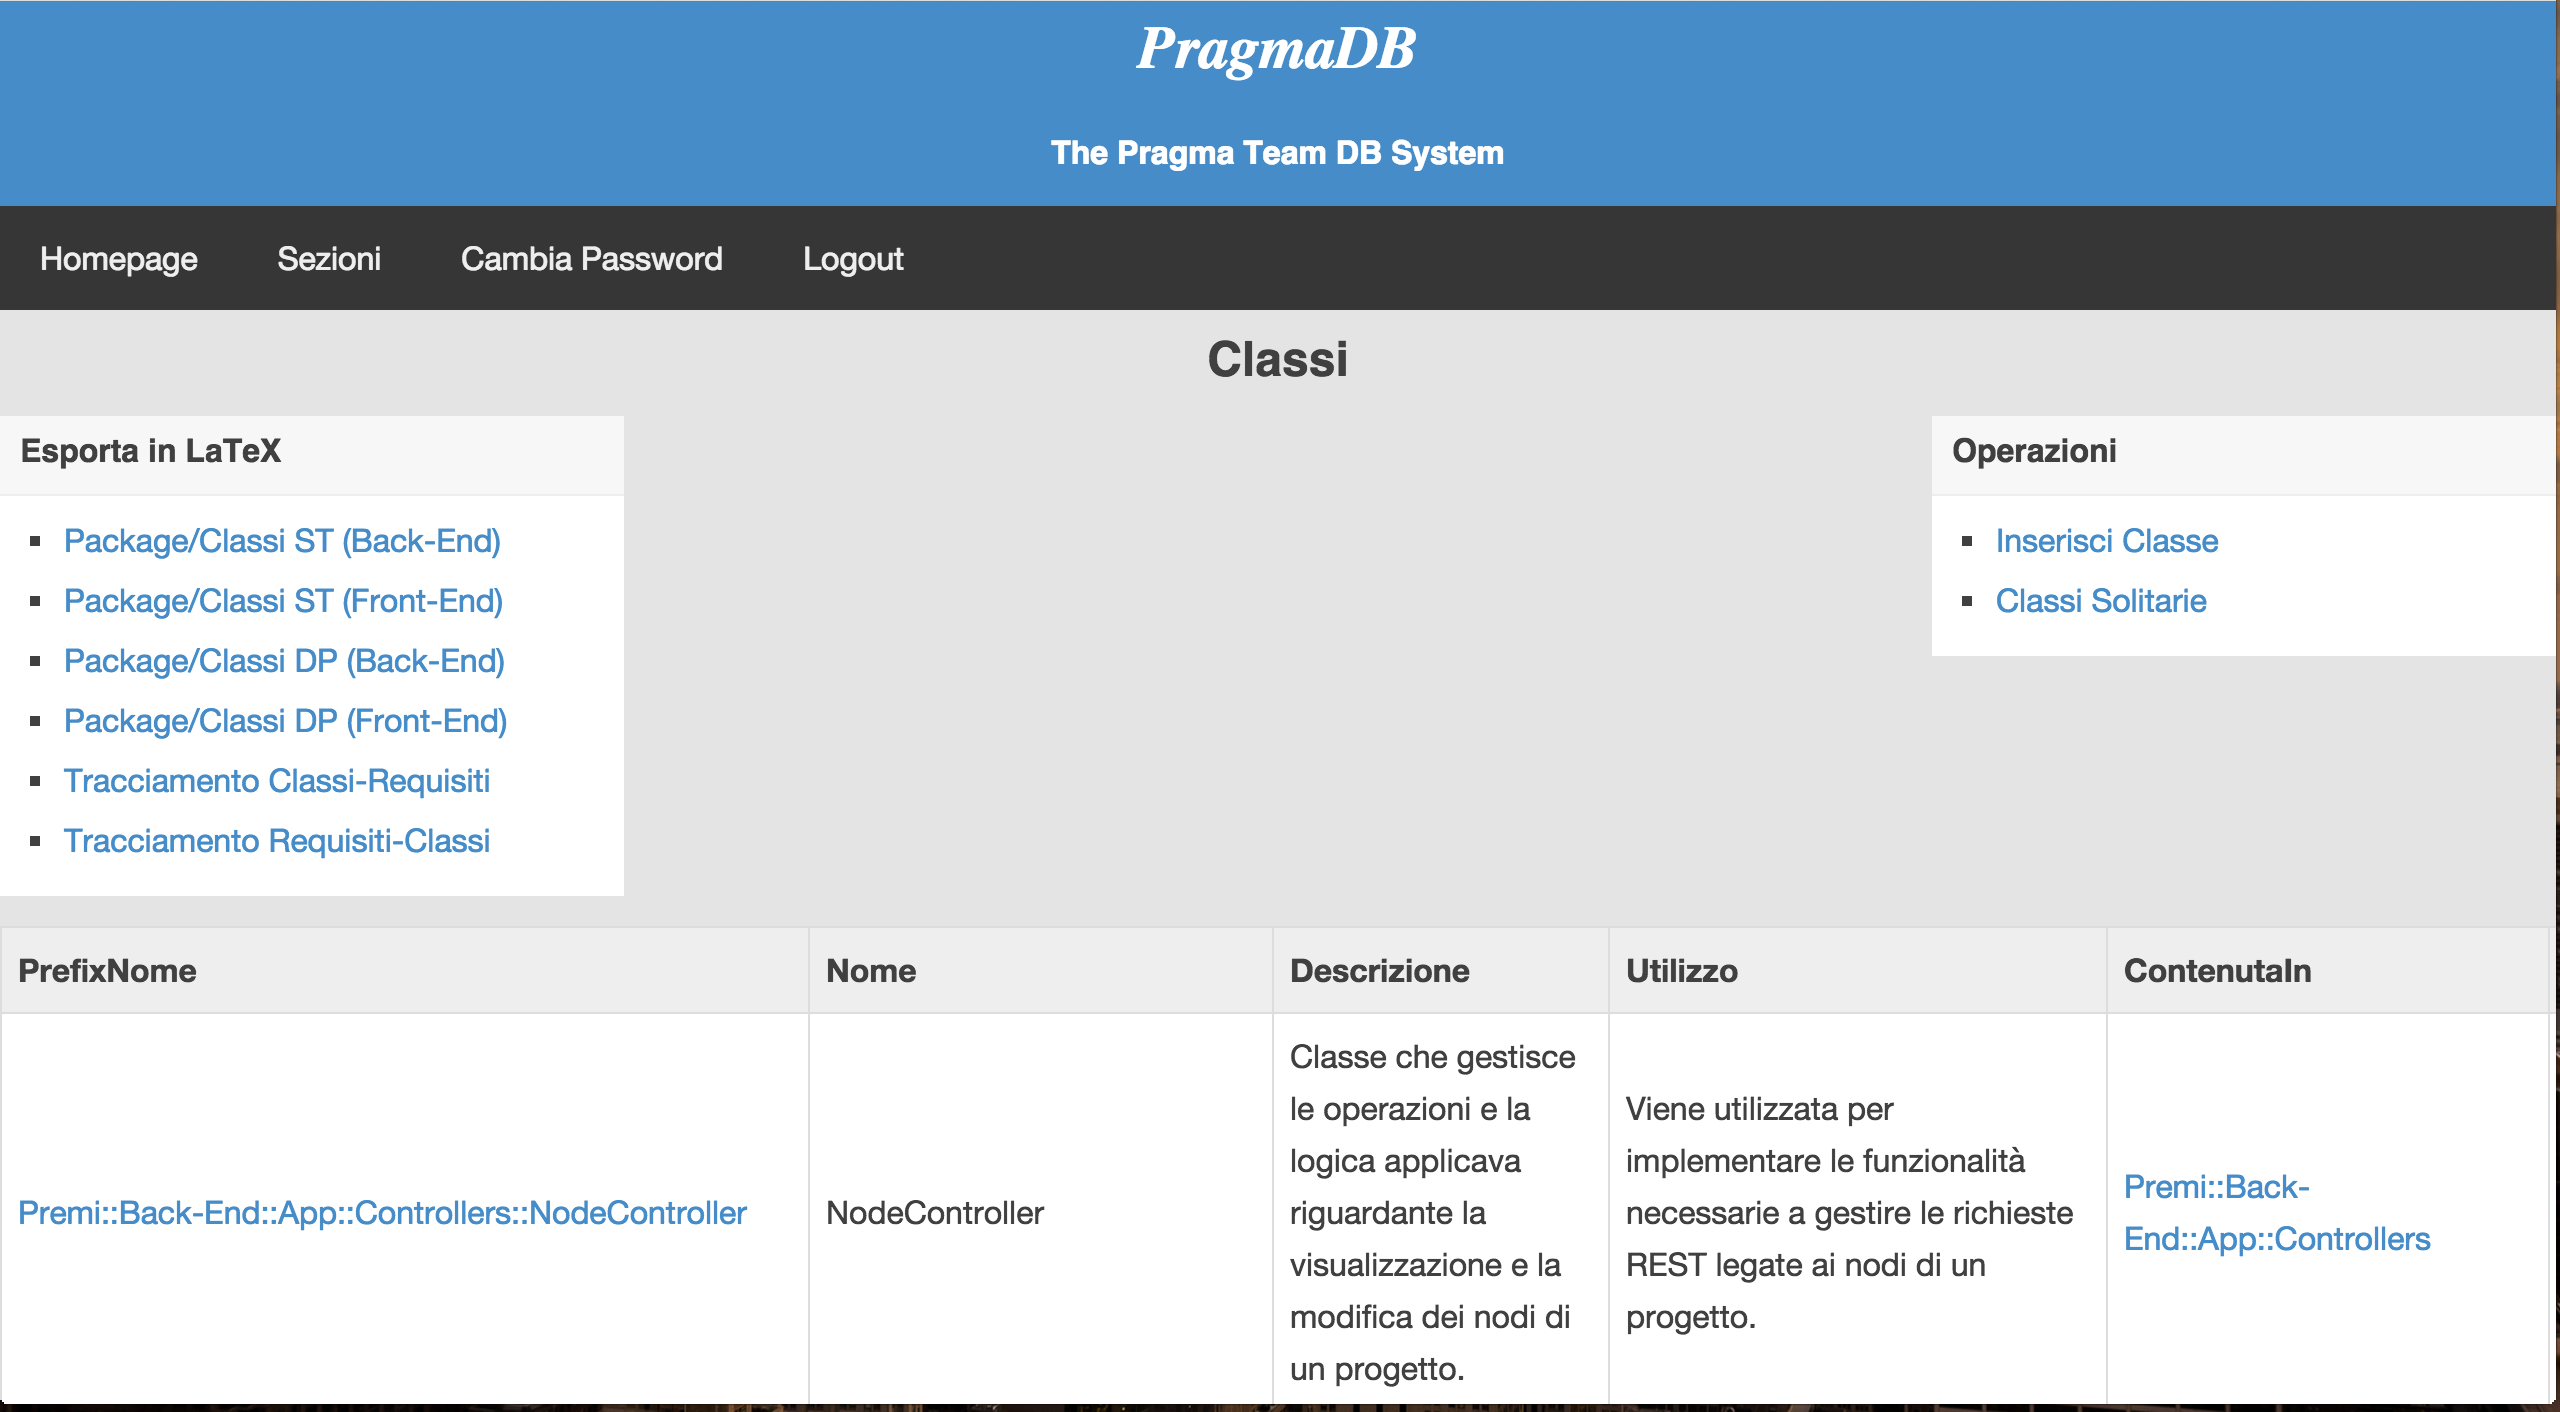
\includegraphics[width=\textwidth,keepaspectratio]{../immagini/pragmadbClassi.png}
\caption{\pragmadb\ - pagina delle classi}\label{fig: PDBGlossario}
\end{figure}
%---------
\begin{figure}[h]
\centering
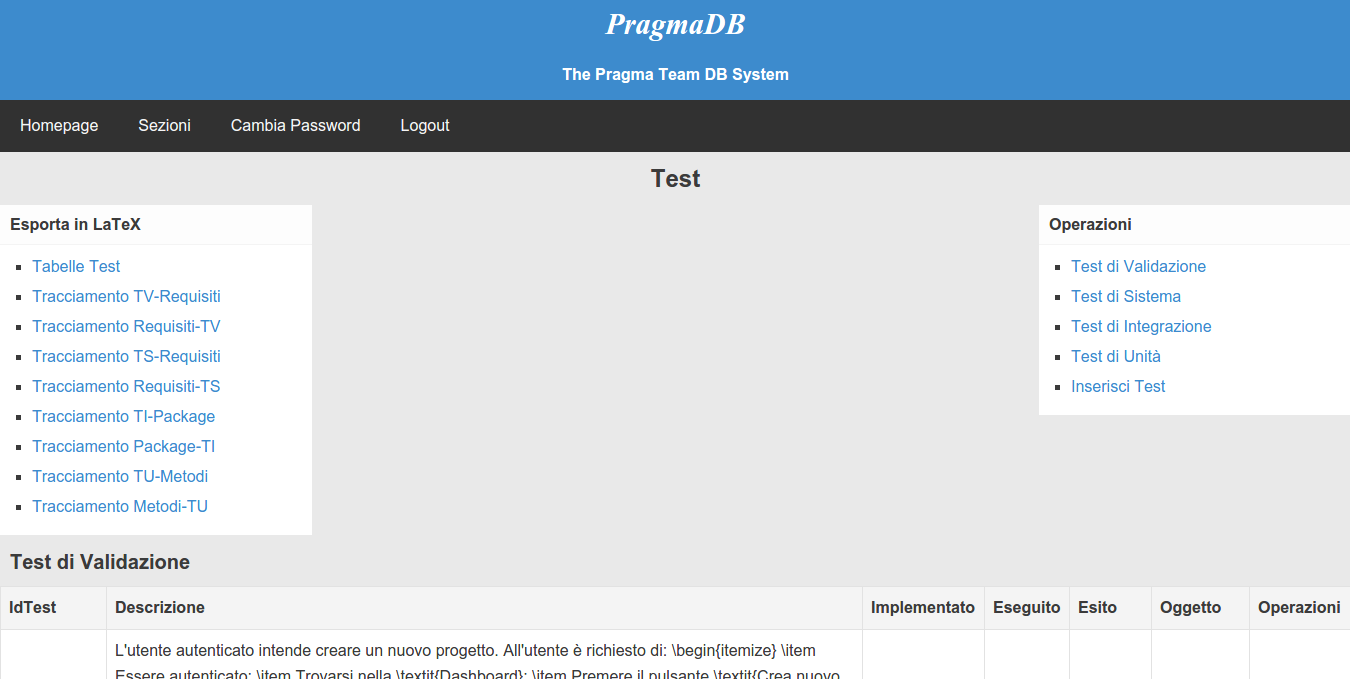
\includegraphics[width=\textwidth,keepaspectratio]{../immagini/pragmadbTest.png}
\caption{\pragmadb\ - pagina dei test}\label{fig: PDBTest}
\end{figure}

\end{appendices}
\end{document}
